\documentclass[dutch,dit,thesis]{hogentreport}

\setlength{\emergencystretch}{3em}

\usepackage{lipsum} % For blind text, can be removed after adding actual content

%% Pictures to include in the text can be put in the graphics/ folder
\graphicspath{{figures/}}

%% For source code highlighting, requires pygments to be installed
%% Compile with the -shell-escape flag!
\usepackage[chapter]{minted}
%% If you compile with the make_thesis.{bat,sh} script, use the following
%% import instead:
%% \usepackage[section,outputdir=../output]{minted}
\usemintedstyle{solarized-light}

%% Formatting for minted environments.
\setminted{%
    autogobble,
    frame=lines,
    breaklines,
    linenos,
    tabsize=4
}

%% Ensure the list of listings is in the table of contents
\renewcommand\listoflistingscaption{%
    \IfLanguageName{dutch}{Lijst van codefragmenten}{List of listings}
}
\renewcommand\listingscaption{%
    \IfLanguageName{dutch}{Codefragment}{Listing}
}
\renewcommand*\listoflistings{%
    \cleardoublepage\phantomsection\addcontentsline{toc}{chapter}{\listoflistingscaption}%
    \listof{listing}{\listoflistingscaption}%
}

% Other packages not already included can be imported here
\usepackage{siunitx}
\usepackage{graphicx}
\usepackage{booktabs}
\usepackage{array}
\usepackage{longtable}
\usepackage{multirow}
\usepackage{float}
\usepackage{caption}
\usepackage{subcaption}
\usepackage{hyperref}
\usepackage{xcolor}
\usepackage{amsmath}
\usepackage{microtype}
\usepackage{parskip}
\usepackage{enumitem}
\usepackage{graphicx}
\usepackage{booktabs}
\usepackage{siunitx}
\usepackage{caption}
\usepackage{subcaption}

\sisetup{
    group-separator={.},
    output-decimal-marker={,},
    per-mode=symbol,
}


%%---------- Document metadata -------------------------------------------------
\author{Jules Van Nevel}
\supervisor{Dhr. A. De Witte}
\cosupervisor{Dhr. S. Verschraege}
\title[]%
    {Ontwikkeling van een herstelmechanisme voor modlaunchers ter preventie van datacorruptie}
\academicyear{\advance\year by -1 \the\year--\advance\year by 1 \the\year}
\examperiod{2}
\degreesought{\IfLanguageName{dutch}{Professionele bachelor in de toegepaste informatica}{Bachelor of applied computer science}}
\partialthesis{false} %% To display 'in partial fulfilment'
%\institution{Internshipcompany BVBA.}

%% Add global exceptions to the hyphenation here
\hyphenation{game-cul-tuur}
\hyphenation{mod-launcher}
\hyphenation{save-game}

%% The bibliography (style and settings are  found in hogentthesis.cls)
\addbibresource{bachproef.bib}            %% Bibliography file
\addbibresource{../voorstel/voorstel.bib} %% Bibliography research proposal
\defbibheading{bibempty}{}

%% Prevent empty pages for right-handed chapter starts in twoside mode
\renewcommand{\cleardoublepage}{\clearpage}

\renewcommand{\arraystretch}{1.2}

%% Content starts here.
\begin{document}

%---------- Front matter -------------------------------------------------------

\frontmatter

\hypersetup{pageanchor=false} %% Disable page numbering references
%% Render a Dutch outer title page if the main language is English
\IfLanguageName{english}{%
    %% If necessary, information can be changed here
    \degreesought{Professionele Bachelor toegepaste informatica}%
    \begin{otherlanguage}{dutch}%
       \maketitle%
    \end{otherlanguage}%
}{}

%% Generates title page content
\maketitle
\hypersetup{pageanchor=true}

%%=============================================================================
%% Voorwoord
%%=============================================================================

\chapter*{\IfLanguageName{dutch}{Woord vooraf}{Preface}}%
\label{ch:voorwoord}

Ik speel al meer dan twaalf jaar Kerbal Space Program. Dat klinkt misschien overdreven, maar wie het spel kent, begrijpt het meteen: KSP is geen gewoon spel. Het is een ruimtevaartsimulator waar je zelf raketten bouwt, missies plant en (als alles goed gaat) succesvol landt op andere planeten. Voor iemand die geïnteresseerd is in raketten en ruimtevaart, is het eigenlijk het perfecte spel.

Mijn primaire KSP installatie is met het echte zonnestelsel nagebootst in het spel, wat een modpack van 130 mods vereist. En wie mods installeert, weet ook wat er vroeg of laat fout gaat: mysterieuze crashes, mods die elkaar tegenwerken, en uren spenderen aan debuggen om uiteindelijk toch opnieuw te beginnen. Dat heb ik in die twaalf jaar meer keren meegemaakt dan ik wil toegeven. Dit probleem is dan ook precies wat ik in deze bachelorproef probeer aan te pakken. Het voelde meteen als een onderwerp waar ik écht iets mee kon doen, niet alleen voor mezelf, maar ook voor de bredere KSP-community.

Graag bedank ik een aantal mensen die dit mogelijk hebben gemaakt. Harvester en Squad verdienen een grote dank voor het creëren van dit unieke spel. De modding-community, en in het bijzonder BallisticFox voor al het werk in de nieuwe versie van de Real Solar System mod, houdt het spel levend lang nadat de officiële ontwikkeling stopte in 2023. Verder hebben YouTubers zoals Scott Manley, Matt Lowne, Everyday Astronaut, CSI Starbase en het NASASpaceflight-team mijn fascinatie voor de ruimte jaar na jaar verder aangewakkerd.

Een bijzonder grote dank aan mijn promotor, dhr.\ Andreas De Witte, en co-promotor, dhr.\ Sion Verschraege. Hun oprechte interesse in het onderwerp en hun waardevolle feedback hebben deze bachelorproef naar een hoger niveau gebracht.

Tot slot wil ik mijn familie en vrienden van harte bedanken. Thuis kon ik altijd rekenen op een luisterend oor als ik vast zat, en me er altijd bovenop hielpen als de stress te groot werd. Ik kon ook altijd rekenen op mijn vrienden voor de leuke game-sessies of gewoon altijd beschikbaar waren om me even af te leiden, jullie weten wie jullie zijn. Zonder die steun was dit een stuk zwaarder geweest.

\bigskip

\noindent Jules Van Nevel, 26 mei 2026
%%=============================================================================
%% Samenvatting
%%=============================================================================

% TODO: De "abstract" of samenvatting is een kernachtige (~ 1 blz. voor een
% thesis) synthese van het document.
%
% Een goede abstract biedt een kernachtig antwoord op volgende vragen:
%
% 1. Waarover gaat de bachelorproef?
% 2. Waarom heb je er over geschreven?
% 3. Hoe heb je het onderzoek uitgevoerd?
% 4. Wat waren de resultaten? Wat blijkt uit je onderzoek?
% 5. Wat betekenen je resultaten? Wat is de relevantie voor het werkveld?
%
% Daarom bestaat een abstract uit volgende componenten:
%
% - inleiding + kaderen thema
% - probleemstelling
% - (centrale) onderzoeksvraag
% - onderzoeksdoelstelling
% - methodologie
% - resultaten (beperk tot de belangrijkste, relevant voor de onderzoeksvraag)
% - conclusies, aanbevelingen, beperkingen
%
% LET OP! Een samenvatting is GEEN voorwoord!

\IfLanguageName{english}{%
\selectlanguage{dutch}
\chapter*{Samenvatting}
\lipsum[1-4]
\selectlanguage{english}
}{}

%%---------- Samenvatting -----------------------------------------------------
% De samenvatting in de hoofdtaal van het document

\chapter*{\IfLanguageName{dutch}{Samenvatting}{Abstract}}

Wie mods installeert voor een game zoals Kerbal Space Program, maakt vaak gebruik van een mod-launcher zoals CKAN om installatie en beheer te automatiseren. Deze tools bieden echter geen ingebouwd back-up- of rollbackmechanisme. Wanneer een modinstallatie misloopt door conflicten, verouderde afhankelijkheden of een beschadigde savegame, heeft de gebruiker vaak slechts één optie: het spel volledig herinstalleren, een proces dat vele uren kan kosten en waarbij persoonlijke voortgang verloren kan gaan.

De centrale onderzoeksvraag luidt: \textit{Hoe kan een robuust en efficiënt back-up- en rollbackmechanisme worden ontworpen voor mod-launchers zoals CKAN, zodat dataverlies en corruptie voorkomen kunnen worden zonder negatieve impact op performantie of gebruiksvriendelijkheid?} Het doel is een reeks onderbouwde ontwerprichtlijnen te formuleren en te valideren via een werkend prototype.

Het onderzoek verloopt in drie fasen. Op basis van 47 posts uit de KSP-community, gespreid over twaalf jaar, brengt een eerste probleemanalyse de aard en frequentie van veelvoorkomende problemen in kaart. Vervolgens worden vier back-upmethodes en zeven compressie-algoritmes vergeleken via metingen op snelheid, opslaggebruik en systeembelasting. Ten slotte wordt een \textit{standalone} Python-prototype gebouwd en geëvalueerd met behulp van een functionele testmatrix, een conformiteitscheck en een heuristische UI-analyse.

De probleemanalyse bevestigt dat crashende installaties door modconflicten en beschadigde savegames structurele, wijdverspreide problemen zijn waarvoor geen geïntegreerde oplossing bestaat. Uit de technische analyse komt btrfs-snapshotting naar voren als de meest aantrekkelijke methode op ondersteunde bestandssystemen, op andere systemen biedt incrementele tar in combinatie met \texttt{zstd}-compressie de beste afweging. Opvallend is dat \texttt{zstd} op grote werklasten sneller is dan ongecomprimeerde tar, terwijl de opslagwinst op de geteste modset circa 53 procent bedraagt. Het prototype toont dat deze aanpak praktisch realiseerbaar is: een back-up van een KSP-installatie van 20{,}5~GB met 113 mods voltooit in ongeveer 37{,}5 seconden, een restore in circa 25 seconden, terwijl de gebruikersinterface responsief blijft.

Uit het onderzoek vloeien vier kernprincipes voort: een gelaagde methodekeuze op basis van het beschikbare bestandssysteem, compressie als integraal onderdeel van het ontwerp, lokale werking zonder netwerkafhankelijkheid, en voorspelbaarheid als centrale kwaliteit van de gebruikersinterface. De geformuleerde richtlijnen bieden een direct toepasbare basis voor ontwikkelaars van mod-launchers.


%---------- Inhoud, lijst figuren, ... -----------------------------------------

\tableofcontents

% In a list of figures, the complete caption will be included. To prevent this,
% ALWAYS add a short description in the caption!
%
%  \caption[short description]{elaborate description}
%
% If you do, only the short description will be used in the list of figures

\listoffigures

% If you included tables and/or source code listings, uncomment the appropriate
% lines.
\listoftables

\listoflistings

\chapter*{\IfLanguageName{dutch}{Lijst van afkortingen}{List of abbreviations}}
\addcontentsline{toc}{chapter}{\IfLanguageName{dutch}{Lijst van afkortingen}{List of abbreviations}}
\begin{description}[labelwidth=2cm, leftmargin=2.5cm, style=sameline]
    \item[btrfs]  B-tree File System
    \item[BWT]    Burrows-Wheeler Transformatie
    \item[CKAN]   Comprehensive Kerbal Archive Network
    \item[CDP]    Continue Dataprotectie
    \item[CPU]    Central Processing Unit
    \item[ext4]   Fourth Extended Filesystem
    \item[FSE]    Finite State Entropy
    \item[GB]     Gigabyte
    \item[GPU]    Graphics Processing Unit
    \item[I/O]    Input/Output
    \item[KDE]    K Desktop Environment
    \item[KSP]    Kerbal Space Program
    \item[LZ77]   Lempel-Ziv 77
    \item[LZMA]   Lempel-Ziv-Markov Chain Algorithm
    \item[MB]     Megabyte
    \item[NTFS]   New Technology File System
    \item[NVMe]   Non-Volatile Memory Express
    \item[PoC]    Proof of Concept
    \item[RAM]    Random Access Memory
    \item[RSS]    Resident Set Size
    \item[SSD]    Solid State Drive
    \item[UI]     User Interface
    \item[UX]     User Experience
    \item[zfs]    Zettabyte File System
    \item[zstd]   Zstandard
\end{description}

%---------- Kern ---------------------------------------------------------------

\mainmatter{}

% De eerste hoofdstukken van een bachelorproef zijn meestal een inleiding op
% het onderwerp, literatuurstudie en verantwoording methodologie.
% Aarzel niet om een meer beschrijvende titel aan deze hoofdstukken te geven of
% om bijvoorbeeld de inleiding en/of stand van zaken over meerdere hoofdstukken
% te verspreiden!

\input{inleiding}
\input{standvanzaken}
\input{methodologie}

% Voeg hier je eigen hoofdstukken toe die de ``corpus'' van je bachelorproef
% vormen. De structuur en titels hangen af van je eigen onderzoek. Je kan bv.
% elke fase in je onderzoek in een apart hoofdstuk bespreken.

\chapter{\IfLanguageName{dutch}{Probleemanalyse en dataverzameling}{Problemanalysis and datacollection}}%
\label{ch:probleemanalyse}

\section{Overzicht van de dataset}

Voor dit onderzoek werden in totaal 47 posts geanalyseerd, afkomstig van Reddit, Steam Community, het officiële KSP-forum en platformen zoals StackExchange en GitHub. Deze posts zijn verspreid over een periode van 12 jaar, wat meteen een eerste belangrijke vaststelling illustreert: de problemen die spelers ondervinden bij het gebruik van modlaunchers zijn niet nieuw, en zijn doorheen de volledige levenscyclus van KSP blijven terugkeren.

\section{Meest voorkomende probleemtypes}

\subsection{Crashes door modconflicten, verouderde mods of ontbrekende afhankelijkheden}

Dit is het meest gerapporteerde probleem in de dataset. Het gaat om crashes tijdens het laden van het spel, bij het openen van een savegame, of willekeurig tijdens gameplay. De oorzaak ligt zelden bij één enkele mod, maar bij de interactie tussen meerdere mods of bij een versie-incompatibiliteit. Voorbeelden hiervan zijn crashes door de mod TweakScale na een CKAN-update en crashes omtrent de B9 Part Switch mod.

Een opvallend patroon is dat gebruikers soms melden dat een herinstallatie van de mod het probleem niet oplost. De reden daarvoor kan liggen aan het feit dat deze problemen veroorzaakt worden door meerdere mods of overlappende configuratiebestanden in de GameData-map, die de nieuwe installatie blijven verstoren. Dit probleem doet zich voor zowel bij manuele installaties als bij installaties via CKAN.

\subsection{Corrupte of verloren savegames}

Een tweede veelvoorkomend probleem betreft beschadigde of onherstelbare savegamebestanden. De oorzaken zijn divers: een stroomonderbreking tijdens het opslaan, een bluescreen door RAM-problemen, een automatische KSP-update terwijl er actieve vluchten in de savegame zaten, of een antivirusprogramma (Avast) dat savebestanden als verdacht beschouwde en verwijderde. In één geval raakte een save beschadigd simpelweg door het laden van het spel na een modwijziging.

Het centrale bestand bij dit probleemtype is persistent.sfs, het primaire savegamebestand van KSP. Wanneer dit bestand corrupt raakt of verdwijnt, is de savegame onbruikbaar. KSP maakt automatisch backups aan in een /saves/<savegame>/Backup-submap en als de gebruiker manueel de game opslaat wordt er een quicksave.sfs gemaakt. Deze zorgen ervoor dat veel savegame corrupties opgelost kunnen worden, maar het probleem is dat de meerderheid van de spelers zich hier niet van bewust zijn dat deze bestanden bestaan.

\subsection{Niet ladende mods}

Een derde categorie omvat gevallen waarbij mods via CKAN geïnstalleerd worden, maar vervolgens niet zichtbaar zijn in het spel. De oorzaak is doorgaans een verkeerde installatielocatie, een dubbele installatie van het spel op dezelfde machine, of ontbrekende afhankelijkheden. Dit probleemtype wordt bijna uitsluitend veroorzaakt door gebruikersfouten en is in de meeste gevallen relatief eenvoudig te verhelpen.

\subsection{Te kort aan geheugen}

Een minder zichtbaar maar terugkerend probleem is het te kort aan werkgeheugen. KSP is een geheugenintensief spel, en zeker bij uitgebreide modpacks kan de geheugengrens snel bereikt worden. Dit manifesteert zich als willekeurige crashes tijdens gameplay of bij het laden, zonder duidelijke foutmelding. Meerdere posts in de dataset vermelden expliciet dat een laptop met 8 GB RAM waarschijnlijk te weinig is, of dat het verwijderen van niet-essentiële mods de stabiliteit verbetert. Doordat de oorzaak niet direct zichtbaar is in de logs, worden deze problemen vaak laat of nooit correct geïdentificeerd.

\section{Oorzaken: gebruikersfout of systeemfout?}

Van de 47 geanalyseerde posts werden 19 posts geclassificeerd als (mede) veroorzaakt door een gebruikersfout. Het gaat daarbij om acties zoals het manueel verwijderen van bestanden uit de GameData-map zonder te controleren welke bestanden cruciaal zijn, het mixen van KSP-versies met incompatibele modversies, het negeren van afhankelijkheden, of het vasthouden aan een verouderde KSP-versie ondanks adviezen om te updaten.

3 posts werden geclassificeerd als een fout van CKAN zelf, waarbij de launcher een update installeerde over bestaande bestanden heen zonder de oude versie eerst te verwijderen.

7 posts vielen onder de categorie "andere oorzaak": hardwarefouten (RAM, stroomuitval), driverproblemen, antivirussoftware, of een verouderde mod buiten de controle van de gebruiker.

De overige posts hadden een onbekende oorzaak, hetzij omdat de oorspronkelijke gebruiker niet terugkeerde om de oplossing te bevestigen, hetzij omdat het probleem nooit werd opgelost.

\section{Aangeboden oplossingen en hun effectiviteit}

\subsection{Meest aangeboden oplossingen}

De meest voorgestelde oplossing over alle probleemtypes heen is een volledige herinstallatie: verwijder alles uit de GameData-map behalve de Squad-mappen, verifieer de spelintegriteit via Steam, en installeer mods opnieuw. Dit is effectief als het probleem wordt veroorzaakt door achtergebleven bestanden, maar het is een destructieve en tijdrovende aanpak die de gebruiker terugzet naar een blanco staat.

Voor savegame-corruptie is de meest effectieve oplossing het herstellen vanuit een backup: hernoem het meest recente backupbestand in /saves/<savegame>/Backup naar persistent.sfs, of hernoem quicksave.sfs door persistent.sfs. Deze aanpak werd in meerdere posts bevestigd als werkend. Het probleem is echter dat gebruikers deze backupmap niet kennen, en dat de backups niet altijd up-to-date zijn op het moment van de crash.

Voor crashproblemen werd ook regelmatig verwezen naar het analyseren van logbestanden (Player.log of KSP.log). Dit is effectief voor het identificeren van de schuldige mod, maar vereist technische kennis die de gemiddelde gebruiker niet heeft. Meerdere helpers in de posts moesten eerst uitleggen waar de logbestanden te vinden zijn.

Een andere veelvoorkomende suggestie is binaire uitsluiting: mods één voor één verwijderen en telkens het spel opnieuw opstarten om te bepalen welke mod het probleem veroorzaakt. Dit werkt, maar is vergt extreem veel tijd bij grote modpacks.

\subsection{Effectiviteit per probleemtype}

Bij crashproblemen door modconflicten zijn oplossingen wisselend effectief. In gevallen waarbij de oorzaak duidelijk geïdentificeerd kon worden (verouderde mod, versie-incompatibiliteit) leidde de gerichte verwijdering of update van die mod tot een oplossing. In gevallen waarbij de oorzaak onduidelijk bleef, bleven gebruikers rondcirkelen met herinstallaties zonder duurzaam resultaat.

Bij savegame-corruptie zijn oplossingen redelijk effectief als er backups beschikbaar zijn. In gevallen zonder backups, door stroomuitval, antivirussoftware of een ontbrekend quicksave-bestand, was het verlies permanent en onherstelbaar.

Bij het probleem van niet-ladende mods waren oplossingen overwegend effectief, omdat de oorzaak doorgaans eenvoudig te identificeren en te verhelpen was.

\section{Jebretary en de nood aan externe tools}

In een bepaalde thread op de KSP-forum werd opgemerkt dat het wenselijk zou zijn om een externe applicatie of editor te hebben die corrupte savebestanden automatisch kan diagnosticeren. Een van de reacties in die thread linkt naar Jebretary, een tool beschikbaar via GitHub, die git gebruikt om wijzigingen in savebestanden bij te houden en elke versie als aparte commit op te slaan.

Jebretary is een interessant vroeg voorbeeld van een back-up- en herstelmechanisme voor KSP-saves. Het maakt het mogelijk om terug te keren naar een eerdere staat van het savebestand, wat savegame-corruptie door crashes of mislukte mod-updates had kunnen voorkomen. Toch kent de tool aanzienlijke beperkingen: ze werd voor het laatst bijgewerkt op 20 augustus 2014, werkt uitsluitend op Windows, en biedt geen oplossing voor bredere problemen zoals incompatibele mods of beschadigde installatiebestanden.

Het bestaan van Jebretary toont aan dat de behoefte aan automatische herstel- en backupmechanismen al vroeg werd gevoeld in de KSP-moddingcommunity. Het feit dat er sindsdien geen volwaardige opvolger is gekomen, en dat gebruikers vandaag de dag nog steeds handmatig persistent.sfs moeten hernoemen of backupmappen moeten doorzoeken, bevestigt dat dit een structureel onopgelost probleem blijft.

\section{Structureel en terugkerend karakter van de problemen}

Een van de meest opvallende conclusies uit de analyse is dat de problemen in de dataset zich uitstrekken over de volledige tijdslijn van KSP, van versie 1.2 en 1.3 tot de meest recente posts uit 2025. Dezelfde probleemtypes komen telkens terug: achtergebleven bestanden na een herinstallatie, savegames die corrupt raken door een crash of een update, crashes door ontbrekende afhankelijkheden. De aangeboden oplossingen zijn ook grotendeels onveranderd gebleven: verwijder GameData, verifieer Steam, herstel vanuit backup.

Dit patroon is kenmerkend voor een structureel probleem: het gaat niet om incidentele fouten van individuele gebruikers, maar om een fundamentele leegte in de betrouwbaarheid van modlaunchers en het spelplatform zelf. Er is geen geïntegreerd herstelmechanisme, er is geen automatische validatie van de installatietoestand, en er is geen gebruiksvriendelijke manier om een beschadigde installatie of savegame te herstellen zonder technische kennis of handmatige tussenkomst.

De bevindingen uit deze communityanalyse onderbouwen daarmee rechtstreeks de probleemstelling van dit onderzoek: het ontbreken van een herstelmechanisme in modlaunchers is geen randgeval, maar een wijdverspreid en structureel probleem dat spelers al sinds het begin van KSP ondervinden.
\chapter{\IfLanguageName{dutch}{Technische analyse}{Technical analysis}}%
\label{ch:technischeanalyse}

\section{Inleiding van de testopzet}
\label{sec:inleiding-testopzet}

In dit hoofdstuk wordt eerst een vergelijking gemaakt van verschillende back-up- en herstelmethodes, toegepast op data die typisch is voor modlaunchers. Het doel is om, op basis van metingen, te bepalen welke strategie het meest geschikt is voor het opslaan van twee fundamenteel verschillende soorten data: \emph{savegames} en \emph{modinstallaties}. In het tweede deel van dit hoofdstuk wordt onderzocht welk compressie-algoritme het meest geschikt is om gecombineerd te worden met de back-upmethodes uit het eerste deel.

\subsection{Geteste back-upmethodes}

Er werden vier strategieën getest:

\begin{itemize}
    \item \textbf{Volledige back-up} (\textit{full}): bij elke back-up wordt de volledige doelmap in een nieuw archief geplaatst.
    \item \textbf{Incrementele back-up} (\textit{incremental}): er wordt eerst een volledige back-up gemaakt, daaropvolgende back-ups bevatten enkel de bestanden die gewijzigd zijn ten opzichte van de vorige back-up. Een herstelactie bestaat uit het sequentieel uitpakken van de volledige back-up en alle incrementen tot aan het gewenste herstelpunt.
    \item \textbf{Differentiële back-up} (\textit{differential}): er wordt eerst een volledige back-up gemaakt, daaropvolgende back-ups bevatten alle bestanden die gewijzigd zijn ten opzichte van de eerste (volledige) back-up. Een herstelactie vereist enkel de volledige back-up en de differentiële back-up van het gewenste punt.
    \item \textbf{Snapshot} (\textit{btrfs snapshot}): het bestandssysteem zelf maakt een copy-on-write snapshot van het subvolume. Er wordt geen archiefbestand aangemaakt. De snapshot deelt initieel alle datablokken met het bronsubvolume en kost in eerste instantie enkel metadata-overhead.
\end{itemize}

Voor \emph{volledig}, \emph{incrementeel} en \emph{differentieel} werd \texttt{tar} ingezet als archiefformaat. Voor de snapshotmethode werd gebruikgemaakt van het \texttt{btrfs}-bestandssysteem.

\subsection{Datasets}
\label{subsec:datasets}

Voor de analyse werden twee datasets gebruikt die representatief zijn voor de werklast van een modlauncher:

\begin{itemize}
    \item \textbf{Savegames} (zes opeenvolgende savepoints, oplopend in grootte van $\sim$70~MB tot $\sim$144~MB): deze dataset simuleert een gebruiker die op verschillende tijdstippen tijdens het spelen van Kerbal Space Program (KSP) zijn savestate wenst op te slaan. \texttt{save\_1} stelt het oudste back-uppunt voor en \texttt{save\_6} het meest recente. De savegames zijn gerelateerd: opeenvolgende saves bevatten grotendeels dezelfde gegevens, met enkel de tussentijds gewijzigde savebestanden als verschil.
    \item \textbf{Grote mods} (drie opeenvolgende modversies van $\sim$1{,}3 tot $\sim$2{,}5~GB): deze dataset simuleert het updaten of terugdraaien van zware modpacks. \texttt{mod\_1} is de oudste versie, \texttt{mod\_3} de meest recente. KSP-mods uit de CKAN-index zijn voornamelijk klein, maar er bestaan modpacks die meerdere gigabytes innemen en niet via CKAN worden verspreid. Voor deze mods is een efficiënte back-up- en rollbackstrategie cruciaal, aangezien een mislukte update de gehele installatie kan beschadigen.
\end{itemize}

In beide datasets vertegenwoordigen de items dus opeenvolgende back-up\-punten in de tijd. Dit is essentieel voor de interpretatie van de incrementele en differentiële metingen: \texttt{save\_1} en \texttt{mod\_1} corresponderen telkens met de \emph{eerste} back-up, die per definitie de volledige basis vormt voor incrementele en differentiële strategieën. Latere back-uppunten bevatten enkel het verschil ten opzichte van respectievelijk de vorige back-up (incrementeel) of de basis-back-up (differentieel).

Per combinatie van methode en compressie-algoritme werden tien opeenvolgende runs uitgevoerd om de invloed van toevallige variatie (bijvoorbeeld door I/O-caching of OS-scheduling) te beperken. Alle cijfers in dit hoofdstuk zijn gemiddelden over deze tien runs. Foutbalken in de figuren stellen de standaardafwijking voor.

\subsection{Compressie-algoritmes}

Voor de tar-gebaseerde methodes werd telkens dezelfde set compressie-opties getest: \texttt{geen compressie}, \texttt{gzip}, \texttt{bzip2}, \texttt{xz}, \texttt{lzma}, \texttt{lzip}, \texttt{lzop} en \texttt{zstd}. Deze algoritmen worden in het tweede deel van dit hoofdstuk hoofdstuk geanalyseerd, in het eerste deel wordt enkel de variant zonder compressie besproken om de zuivere back-upmethode-eigenschappen te isoleren.

\subsection{Testomgeving}

De metingen werden uitgevoerd op een laptop met de volgende specificaties:

\begin{itemize}
    \item \textbf{Processor:} AMD Ryzen 9 5900HS (8 cores, 16 threads).
    \item \textbf{Grafische kaart:} NVIDIA GeForce RTX 3060 Laptop GPU.
    \item \textbf{Geheugencapaciteit:} 24GB.
    \item \textbf{Opslag:} NVMe SSD (model HFM001TD3JX013N), met gemeten sequentiële doorvoer van $\sim$3320~MB/s lezen en $\sim$2050~MB/s schrijven (zie figuur~\ref{fig:ssd-bench}). Random 4K I/O bij hoge wachtrij (Q32T1) bedraagt $\sim$481~MB/s lezen en $\sim$277~MB/s schrijven; bij lage wachtrij (Q1T1) bedraagt dit $\sim$56~MB/s lezen en $\sim$116~MB/s schrijven.
\end{itemize}

\begin{figure}[h]
    \centering
    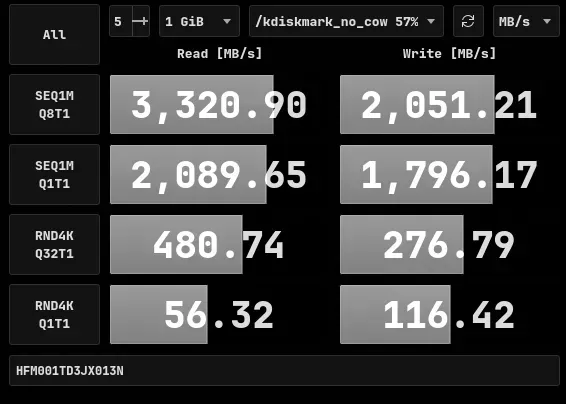
\includegraphics[width=0.6\linewidth]{ssd_stats.png}
    \caption{KDiskMark-resultaten van de gebruikte NVMe SSD.}
    \label{fig:ssd-bench}
\end{figure}

De SSD vormt hier geen knelpunt voor de geteste dataset, zelfs bij de grootste mod ($\sim$2{,}5~GB) zou een sequentiële kopie in theorie binnen één seconde voltooid zijn. Eventuele uitschieters in de meetresultaten zijn dus voornamelijk toe te schrijven aan CPU-werk (archivering, pad-traversal, bestandsmetadata) en niet aan de SSD.

\subsection{Waarom geen cloud-gebaseerde back-up}
\label{subsec:geen-cloud}

In de literatuur over back-upsystemen wordt cloudopslag besproken als een robuuste en geografisch redundante oplossing. Voor de context van modlaunchers, en in het bijzonder voor KSP, is deze aanpak echter niet geschikt:

\begin{itemize}
    \item KSP en de meeste mods werken volledig offline. Veel spelers gebruiken het spel in omgevingen zonder permanente internetverbinding (op verplaatsing, op een laptop in de trein, enz.). Een back-upsysteem dat een actieve verbinding vereist, kan in deze gevallen geen back-up maken op het moment dat dit nodig is, namelijk vlak voor een riskante in-game actie of andere willekeurige corruptie gebeurtenissen.
    \item Mods kunnen meerdere gigabytes groot zijn. Voor een dataset van 2{,}5~GB verwacht een cloud-back-up een upload-bandbreedte die een thuisgebruiker mogelijks niet ter beschikking heeft. De back-up zou daardoor merkbaar trager zijn dan andere back-upmethodes.
    \item Cloudopslag introduceert privacy- en beschikbaarheidsafhankelijkheden van een derde partij, terwijl een lokale back-up volledig onder controle van de gebruiker blijft.
\end{itemize}

Door deze redenen wordt in de rest van dit onderzoek uitgegaan van lokale back-upstrategieën.

\subsection{Betekenis van de meetvelden}
\label{subsec:meetvelden}

Voor elke run werden volgende metrieken vastgelegd:

\begin{description}
    \item[\texttt{time\_s}] De wall clock time, in seconden, tussen het starten en beëindigen van de back-up- of restore-operatie. Voor de restorefase van incrementele en differentiële back-ups is dit de cumulatieve tijd: de tijd die nodig is om alle archieven uit te pakken die nodig zijn om het gewenste back-uppunt volledig terug te zetten. Voor incrementeel betekent dit de basis-back-up plus alle incrementen tot aan het gekozen punt. Voor differentieel betekent dit de basis-back-up plus de differentiële back-up van het gekozen punt.
    \item[\texttt{cpu\_pct}] Het CPU-gebruik zoals gerapporteerd door \texttt{/usr/bin/time}, uitgedrukt als percentage van één CPU-thread. Een waarde van 100\% betekent dat het proces tijdens zijn levensduur gemiddeld één thread volledig benutte. 1400\% komt overeen met het volledige gebruik van veertien threads. Op een 16-thread-CPU is het theoretisch maximum dus 1600\%. Voor single-threaded taken zoals \texttt{tar} zonder multithreaded compressie ligt deze waarde dicht bij 100\%.
    \item[\texttt{mem\_kb}] De maximale RSS (Resident Set Size) van het proces in kilobytes, een proxy voor het piekgeheugengebruik.
    \item[\texttt{size\_original}] De grootte, in bytes, van de bronmap vóór de back-up, gemeten via \texttt{du}.
    \item[\texttt{size\_archive}] De grootte van het resulterende archiefbestand in bytes. Voor btrfs-snapshots is dit veld leeg omdat een snapshot geen archief maakt. De relevante kost wordt daar opgesplitst in twee andere velden.
    \item[\texttt{exclusive\_size}] (enkel snapshots) De hoeveelheid data die strikt eigen is aan deze snapshot, dat wil zeggen niet gedeeld met enige andere snapshot of het bronsubvolume. Deze waarde wordt bekomen via \texttt{btrfs qgroup show}. Bij een verse snapshot is deze grootte minimaal en omvat ze enkel de metadata-overhead.
    \item[\texttt{set\_shared\_size}] (enkel snapshots) De totale grootte van de datablokken die binnen de snapshot-set worden gedeeld. Deze waarde geeft een realistisch beeld van de feitelijke schijfbelasting van de verzameling snapshots: zolang blokken ongewijzigd blijven, kost een bijkomende snapshot nagenoeg geen extra ruimte.
\end{description}

In tegenstelling tot een aggregatie-aanpak waarbij de zes savepoints of drie mods samengeteld  worden tot één totaalwaarde per methode, wordt in dit hoofdstuk de resultaten per individueel back-uppunt gerapporteerd. Deze keuze laat toe om karakteristieke patronen van elke methode bloot te leggen, zoals de zeer goedkope tweede increment of de cumulatieve groei van differentiële archieven, die in een gesommeerde weergave verloren zouden gaan.


\section{Resultaten: back-upfase}
\label{sec:results-backup}

\subsection{Snelheid van de back-up}
\label{subsec:backup-time}

Figuur~\ref{fig:backup-time} toont de back-uptijd per individueel back-uppunt. De vier methodes tonen onderling sterk verschillende patronen.

\begin{figure}[h]
    \centering
    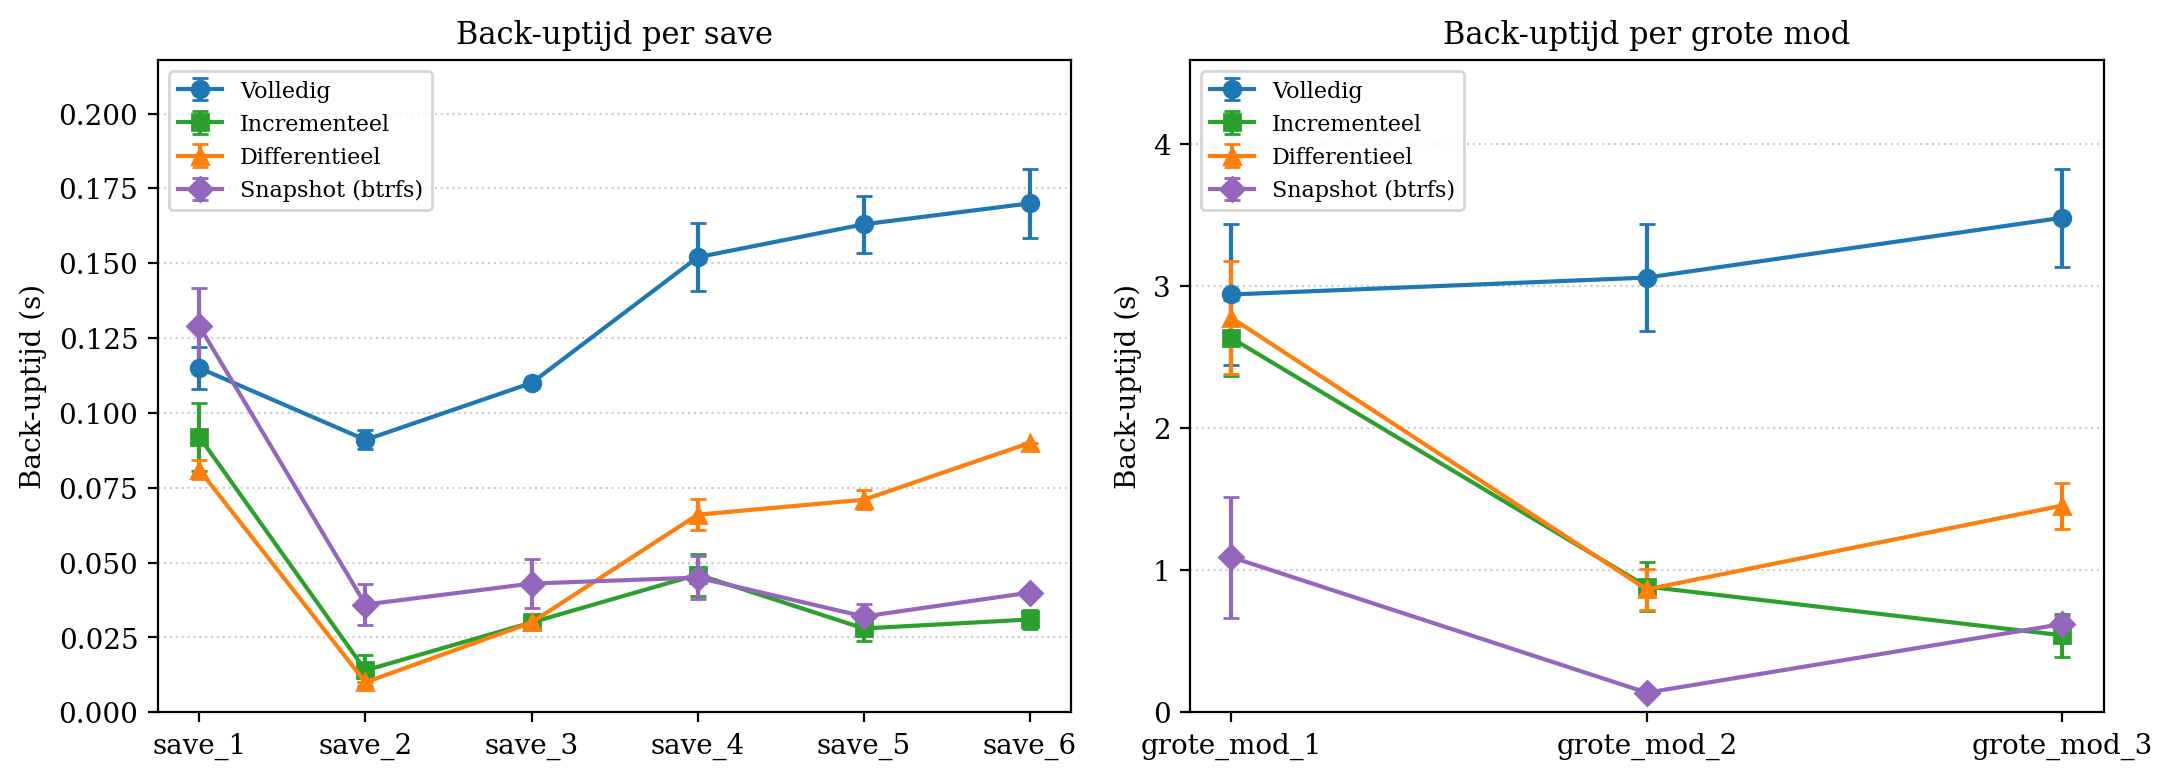
\includegraphics[width=\linewidth]{figures/fig_backup_time_per_point.png}
    \caption{Back-uptijd per individueel back-uppunt (gemiddelde over 10 runs, foutbalken: standaardafwijking). \textbf{Let op:} de y-assen verschillen sterk in schaal omdat de moddataset twee orden van grootte groter is dan de savedataset.}
    \label{fig:backup-time}
\end{figure}

\paragraph{Volledige back-up.}
Bij beide datasets stijgt de back-uptijd voor de volledige methode nagenoeg monotoon met de grootte van de te archiveren folder. Bij de saves stijgt de tijd van $\sim$0{,}11~s voor \texttt{save\_1} tot $\sim$0{,}17~s voor \texttt{save\_6}, in lijn met het feit dat \texttt{save\_6} ongeveer dubbel zo groot is als \texttt{save\_1}. Bij de mods volgt de tijd dezelfde tendens ($\sim$2{,}94~s voor \texttt{mod\_1} tot $\sim$3{,}48~s voor \texttt{mod\_3}). Het belangrijke inzicht is dat de tijd bij de volledige methode niet afhankelijk is van eerdere back-uppunten: elke back-up is een onafhankelijke, volledige kopie en de kost wordt enkel bepaald door de huidige grootte.

\paragraph{Incrementele back-up.}
Bij de saves toont de incrementele methode het meest karakteristieke gedrag. \texttt{save\_1} kost $\sim$0{,}09~s — vrijwel identiek aan de volledige back-up van diezelfde save, want het is per definitie hetzelfde volledige basisarchief. \texttt{save\_2} valt vervolgens terug naar slechts $\sim$0{,}014~s, zes keer sneller dan \texttt{save\_1}. Dit geeft de kerneigenschap van de incrementele strategie weer: \texttt{save\_2} verschilt zeer weinig van \texttt{save\_1} en het increment bevat dus nauwelijks data. Vanaf \texttt{save\_3} schommelt de tijd tussen $\sim$0{,}03~s en $\sim$0{,}05~s, afhankelijk van het volume aan tussentijdse wijzigingen. \texttt{save\_4} ligt duidelijk hoger dan de andere savepunten, wat overeen komt met een groter increment-archief op datzelfde punt (zie verder, sectie~\ref{subsec:storage}). Bij de mods is hetzelfde patroon zichtbaar: \texttt{mod\_1} duurt $\sim$2{,}63~s als basisarchief, \texttt{mod\_2} valt terug naar $\sim$0{,}88~s en \texttt{mod\_3} naar slechts $\sim$0{,}54~s.

\paragraph{Differentiële back-up.}
Voor de differentiële methode is \texttt{save\_2} (en \texttt{mod\_2}) even goedkoop als bij de incrementele methode. Er is op dat moment nog geen verschil tussen ``ten opzichte van de basis'' en ``ten opzichte van de vorige''. Vanaf het derde back-uppunt divergeren de twee methodes wel. Bij de saves stijgt de differentiële back-uptijd van $\sim$0{,}03~s (\texttt{save\_3}) tot $\sim$0{,}09~s (\texttt{save\_6}), terwijl de incrementele tijd in dezelfde range schommelt rond $\sim$0{,}03~s. Bij de mods is het verschil duidelijker: \texttt{mod\_3} kost $\sim$1{,}45~s differentieel tegenover $\sim$0{,}54~s incrementeel. Dit komt doordat de differentiële methode telkens alle wijzigingen ten opzichte van de basis-back-up moet meenemen, waardoor de archieven cumulatief groeien naarmate er meer back-ups worden gemaakt.

\paragraph{Snapshot.}
De snapshotmethode vertoont een fundamenteel ander gedrag. Bij de saves kost de eerste snapshot ($\sim$0{,}13~s) iets meer dan de daarop volgende ($\sim$0{,}03 -- 0{,}05~s). Dit is vermoedelijk te wijten aan het initialiseren van quota-administratie van het bestandssysteem. Vanaf \texttt{save\_2} is de tijd nagenoeg constant en grotendeels onafhankelijk van de grootte van de save. Bij de mods is hetzelfde patroon zichtbaar, met opmerkelijke uitschieters: \texttt{mod\_2} wordt in $\sim$0{,}14~s gesnapshot, acht keer sneller dan \texttt{mod\_1}. Deze uitschieter is mogelijk te wijten aan I/O-caching tussen opeenvolgende runs (de blokken van \texttt{mod\_2} bevinden zich nog in het page cache na de back-up van \texttt{mod\_1}). De brede foutbalk bij \texttt{mod\_1} bevestigt dat de eerste snapshot in een sessie meer variabiliteit vertoont. Wat wel consistent is, is dat de snapshotmethode in geen enkel geval afhangt van het cumulatieve werk van eerdere back-uppunten.

\subsection{CPU-gebruik tijdens de back-up}
\label{subsec:backup-cpu}

Figuur~\ref{fig:backup-cpu} toont het CPU-gebruik per back-uppunt.

\begin{figure}[h]
    \centering
    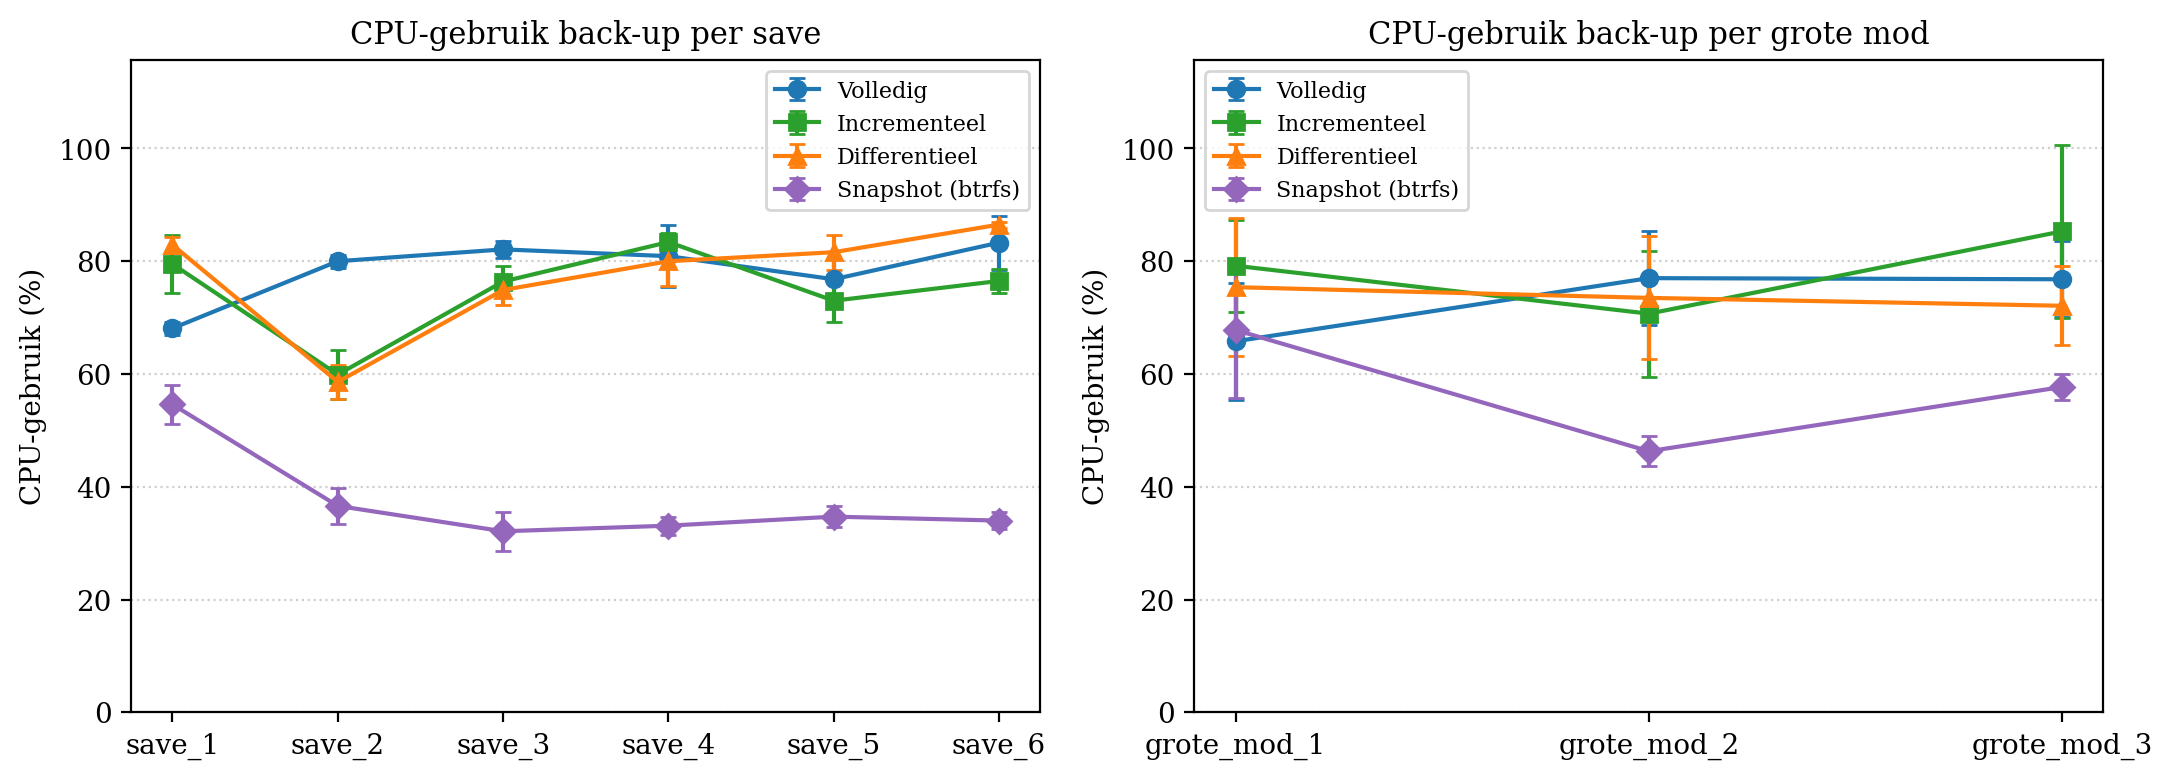
\includegraphics[width=\linewidth]{figures/fig_backup_cpu_per_point.png}
    \caption{CPU-gebruik tijdens de back-upfase, per individueel back-uppunt. De y-as is voor beide grafieken gelijkgeschaald. Een waarde van 100\% komt overeen met één volledige thread; het maximum op deze 16-thread-CPU is 1600\%.}
    \label{fig:backup-cpu}
\end{figure}

Voor de tar-gebaseerde methodes ligt het CPU-gebruik consistent tussen $\sim$60\% en $\sim$85\%. Bij de saves valt op dat \texttt{save\_2} bij zowel incrementeel als differentieel een lager CPU-gebruik toont ($\sim$60\%). Wanneer het increment zeer klein is en de operatie slechts $\sim$10~ms duurt, domineert de opstartoverhead van \texttt{tar} en hoeft de eigenlijke verwerking nauwelijks rekenwerk. Voor de mods, waar elke operatie ten minste een halve seconde duurt, ligt de CPU-utilisatie stabieler tussen 65\% en 85\%.

De snapshotmethode toont een lager CPU-gebruik (25--70\%). Het aanmaken van een btrfs-snapshot is grotendeels een metadata-operatie die in de kernel wordt afgehandeld, het user-space proces (\texttt{btrfs subvolume snapshot}) is zeer kort actief.

\subsection{Geheugengebruik}
\label{subsec:backup-mem}

Figuur~\ref{fig:backup-mem} toont het piek-RSS per back-uppunt.

\begin{figure}[h]
    \centering
    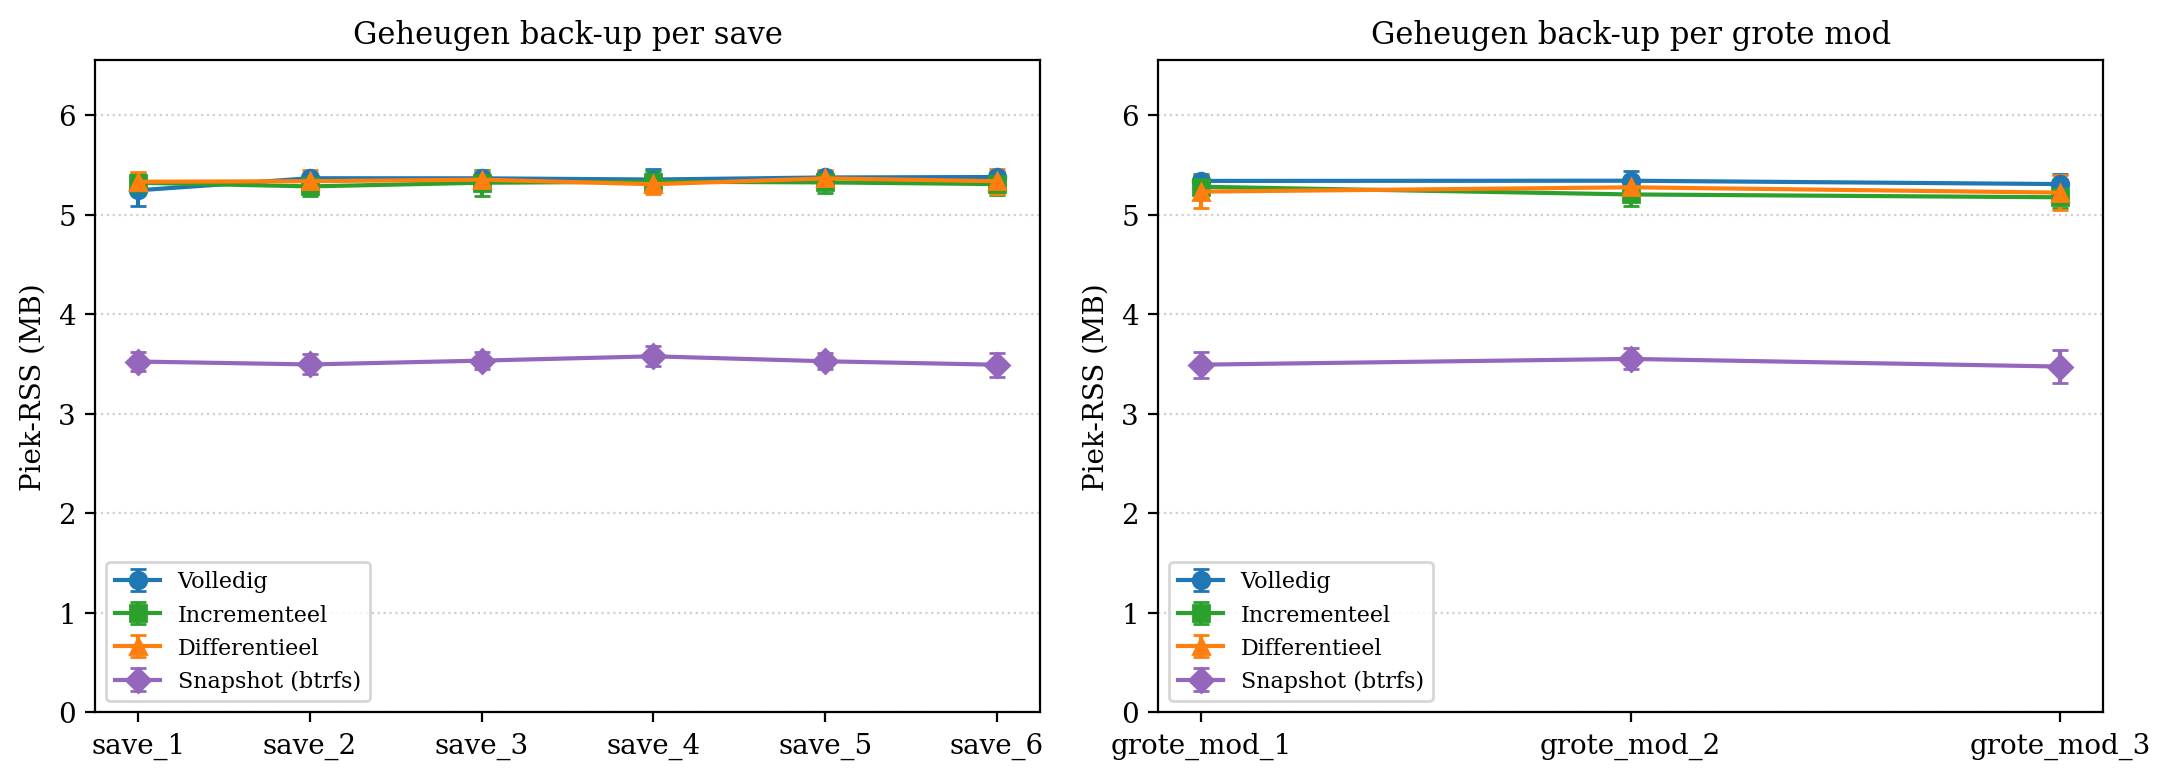
\includegraphics[width=\linewidth]{figures/fig_backup_mem_per_point.png}
    \caption{Piek-RSS van het back-upproces, per individueel back-uppunt. De y-as is identiek geschaald voor beide datasets.}
    \label{fig:backup-mem}
\end{figure}

Het geheugengebruik blijkt onafhankelijk van zowel de methode als de grootte van het te archiveren item. Alle tar-runs liggen tussen 5{,}3 en 5{,}5~MB; de snapshot-runs liggen telkens rond de 3{,}6~MB. \texttt{tar} streamt de invoer en houdt geen volledig archief in het geheugen, waardoor het geheugengebruik niet verschilt op basis van de archief grootte. Op moderne systemen vormt geheugen geen bottleneck voor deze werklast. Wat wel opvalt is dat het geheugengebruik van de snapshotmethode een stuk lager ligt. Dit toont nog eens aan hoe weinig werk een snapshot nemen inhoudt.

\subsection{Opslaggebruik}
\label{subsec:storage}

Figuur~\ref{fig:storage} toont de archiefgrootte per back-uppunt voor de drie tar-methodes. Voor de snapshotmethode wordt de opslag apart besproken in figuren~\ref{fig:snapshot-storage-saves} en~\ref{fig:snapshot-storage-mods}, omdat het concept van ``archiefgrootte'' daar niet van toepassing is.

\begin{figure}[h]
    \centering
    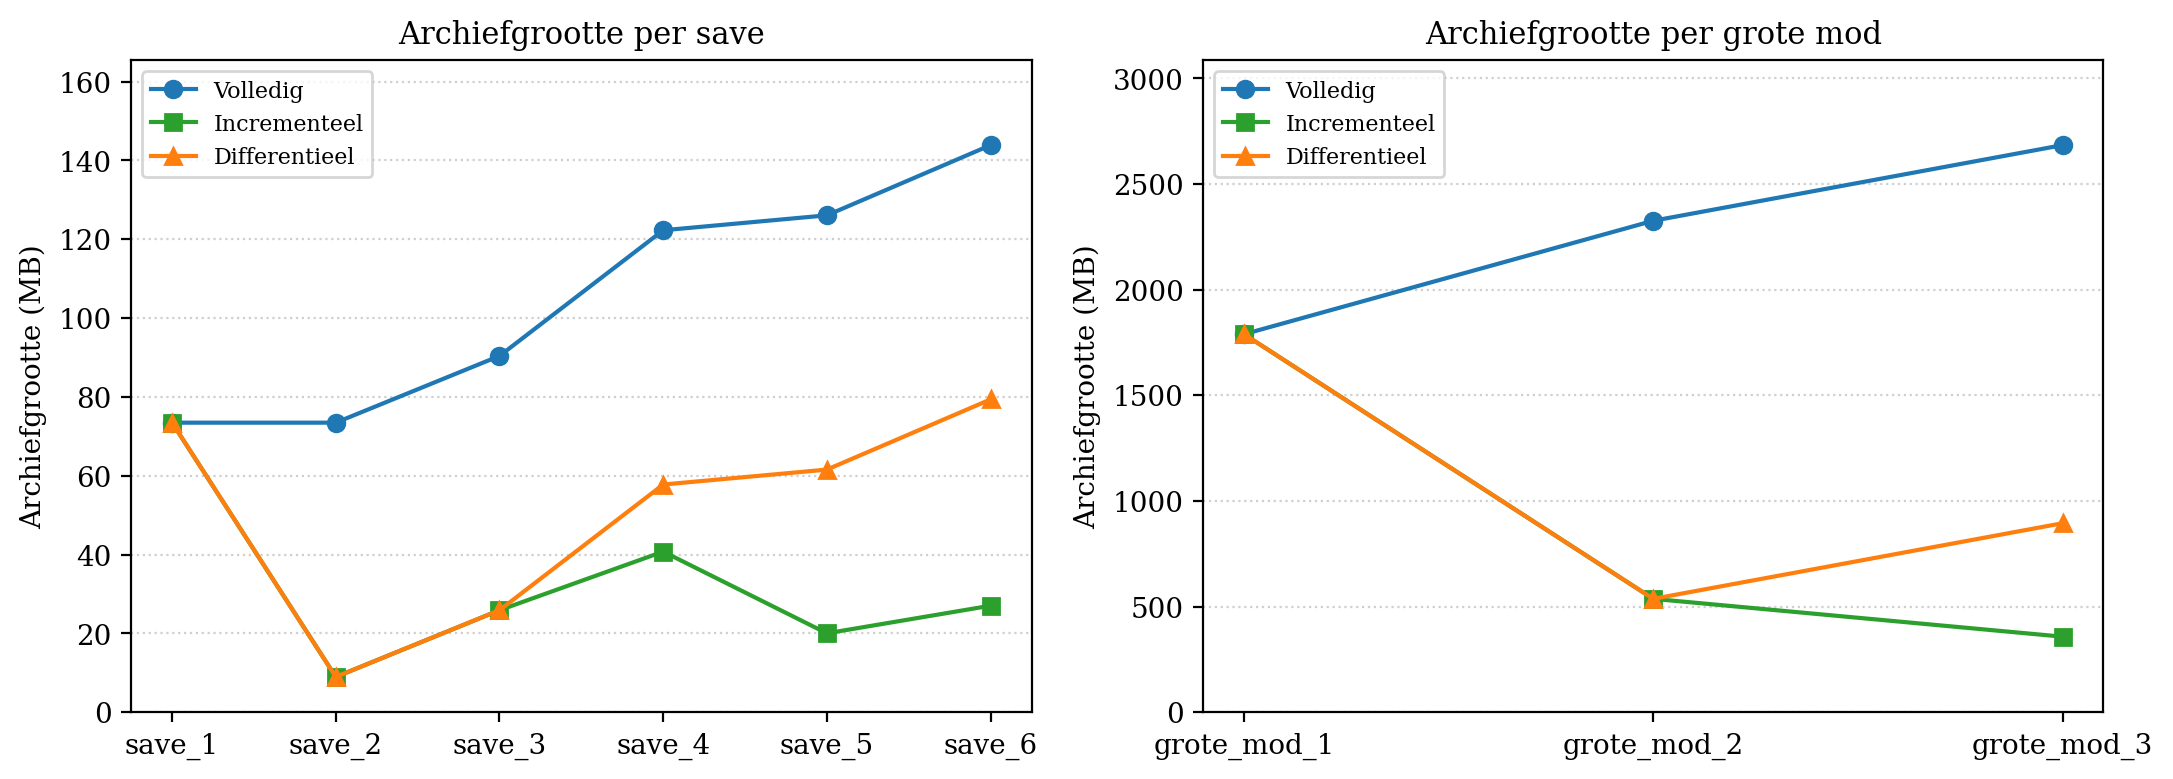
\includegraphics[width=\linewidth]{figures/fig_storage_per_point.png}
    \caption{Archiefgrootte per individueel back-uppunt voor de tar-gebaseerde methodes.}
    \label{fig:storage}
\end{figure}

\paragraph{Volledige back-up.}
Bij de saves stijgt de archiefgrootte van $\sim$73~MB (\texttt{save\_1}) tot $\sim$144~MB (\texttt{save\_6}) en bij de mods van $\sim$1{,}79~GB (\texttt{mod\_1}) tot $\sim$2{,}68~GB (\texttt{mod\_3}). Elke back-up bevat de volledige actuele broninhoud, zonder enige optimalisatie tussen back-uppunten. De cumulatieve opslaggrootte is dus gelijk aan de som van alle balken: ongeveer 630~MB voor de zes saves en 6{,}80~GB voor de drie mods.

\paragraph{Incrementele back-up.}
De grafiek toont het kenmerkende patroon van de incrementele methode. \texttt{save\_1} (en \texttt{mod\_1}) is volledig en daardoor identiek in grootte aan de volledige back-up. \texttt{save\_2} valt terug naar slechts $\sim$9~MB. Daarna fluctueert de archiefgrootte met de hoeveelheid tussentijdse wijzigingen: \texttt{save\_4} geeft een piek ($\sim$41~MB), wat correspondeert met een grotere speelsessie met meer wijzigingen. Bij de mods levert \texttt{mod\_2} een increment van $\sim$537~MB en \texttt{mod\_3} slechts $\sim$358~MB op: de update naar mod-versie 3 bevat dus minder gewijzigde data dan de update naar versie 2. De cumulatieve opslagvoetafdruk komt op $\sim$196~MB voor de saves (een besparing van 69\% ten opzichte van de volledige methode) en $\sim$2{,}68~GB voor de mods (besparing van 60\%).

\paragraph{Differentiële back-up.}
Het verschil met incrementeel wordt onmiddellijk duidelijk. Voor \texttt{save\_2} en \texttt{mod\_2} is de archiefgrootte identiek aan de incrementele variant, omdat het differentieel op dat moment gelijk is aan het increment. Vanaf het derde back-uppunt divergeert differentieel: \texttt{save\_4} is $\sim$58~MB tegenover $\sim$41~MB incrementeel, en \texttt{save\_6} is $\sim$79~MB tegenover $\sim$27~MB incrementeel. Bij de mods is \texttt{mod\_3} zelfs $\sim$895~MB tegenover $\sim$358~MB incrementeel, een verschil van bijna 540~MB voor hetzelfde back-uppunt. Cumulatief loopt dit op tot $\sim$307~MB voor de saves en $\sim$3{,}22~GB voor de mods.

\paragraph{Snapshot.}
Voor de snapshotmethode wordt de opslag op twee manieren weergegeven in figuren~\ref{fig:snapshot-storage-saves} en~\ref{fig:snapshot-storage-mods}: enerzijds de marginale kost per individuele snapshot (de exclusieve datagrootte), anderzijds de cumulatieve fysieke voetafdruk van de hele snapshot-set naarmate er meer back-uppunten worden toegevoegd.

\begin{figure}[h]
    \centering
    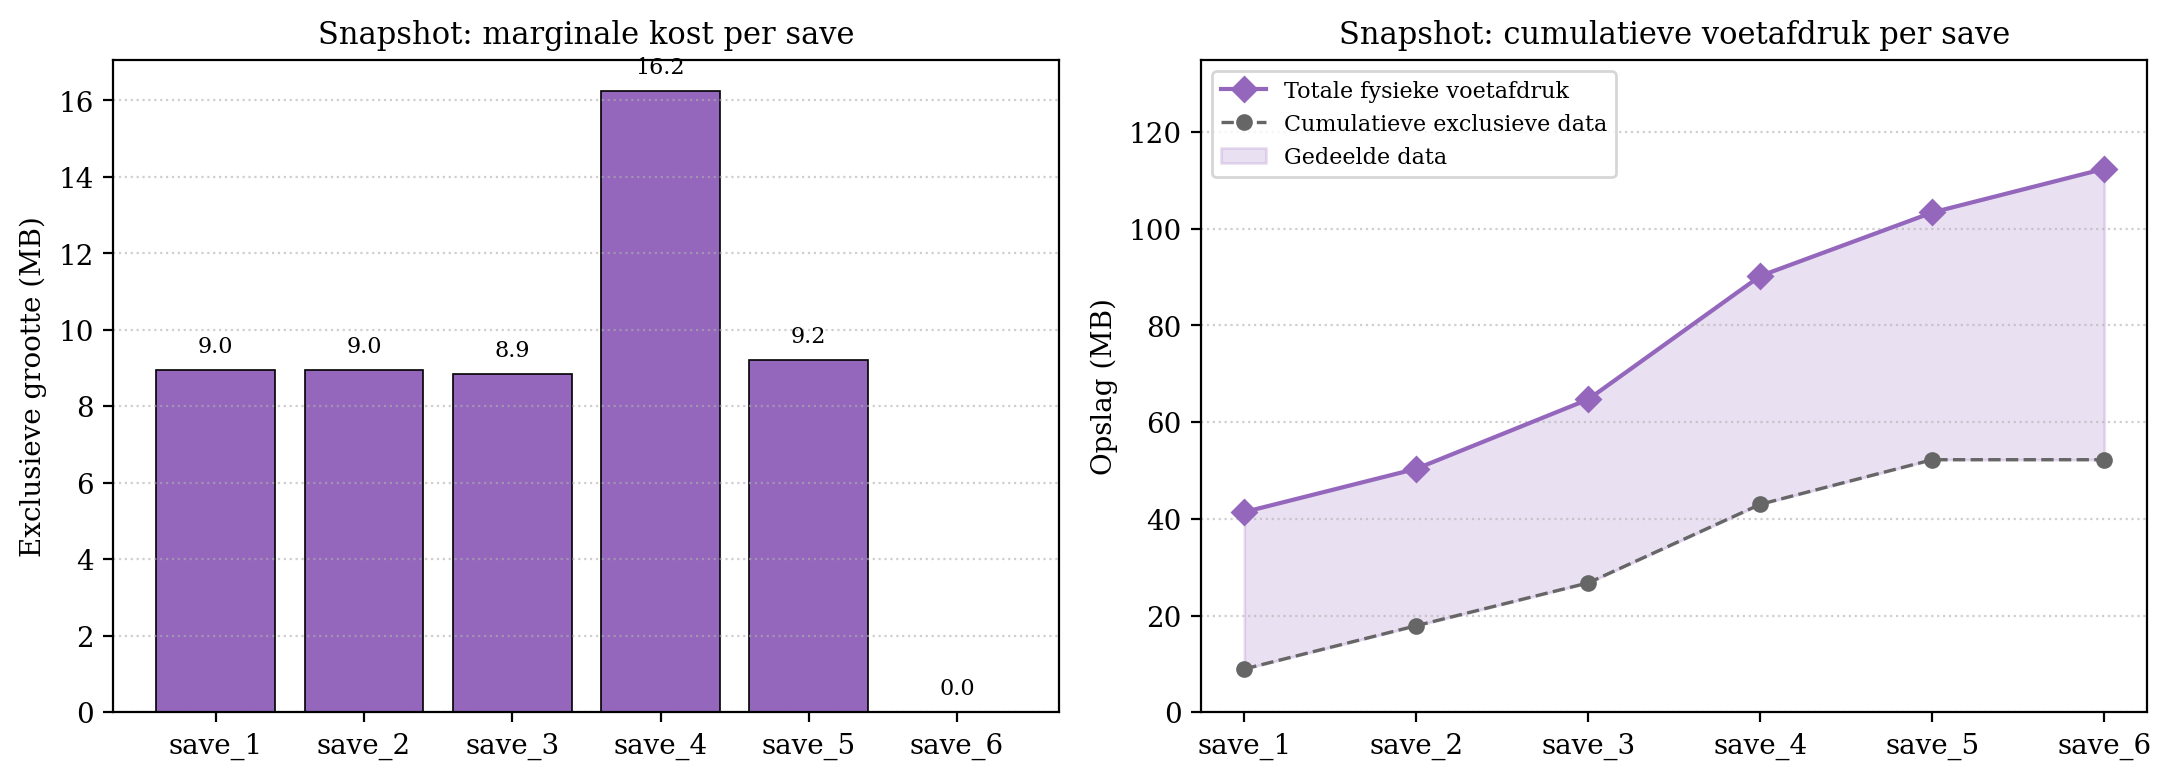
\includegraphics[width=\linewidth]{figures/fig_snapshot_storage_saves.png}
    \caption{Opslagprofiel van de snapshotmethode voor de saves. Links: de marginale kost per snapshot (exclusieve data, dus blokken die niet door andere snapshots of het bronvolume worden gedeeld). Rechts: de totale fysieke voetafdruk van de snapshot-set, opgesplitst in cumulatieve exclusieve data (onderaan) en gedeelde data (gevulde zone).}
    \label{fig:snapshot-storage-saves}
\end{figure}

\begin{figure}[h]
    \centering
    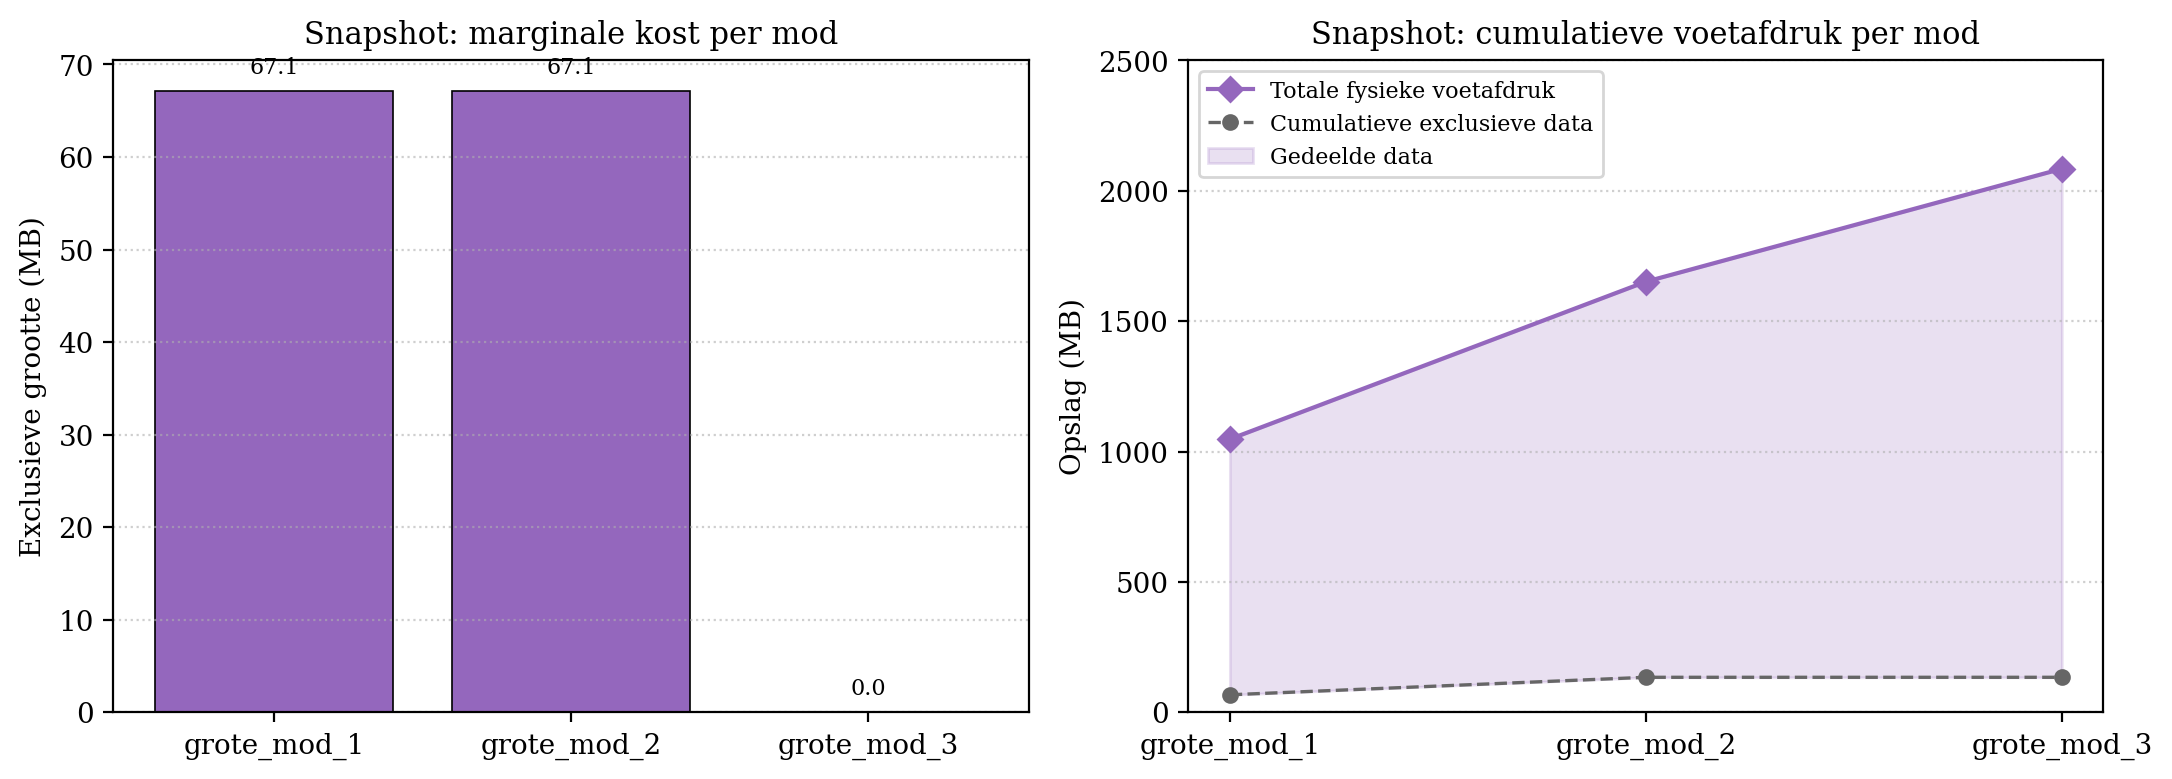
\includegraphics[width=\linewidth]{figures/fig_snapshot_storage_mods.png}
    \caption{Opslagprofiel van de snapshotmethode voor de mods. Zelfde structuur als figuur~\ref{fig:snapshot-storage-saves}.}
    \label{fig:snapshot-storage-mods}
\end{figure}

Bij de saves is de marginale kost per snapshot zeer uniform: elk van de eerste vijf snapshots draagt ongeveer 9~MB aan exclusieve data bij, met één duidelijke uitschieter (\texttt{save\_4}: 16~MB). Deze uitschieter komt opnieuw overeen met de hoger genoemde gameplay-piek tussen \texttt{save\_3} en \texttt{save\_4}: meer gewijzigde blokken impliceert meer data die exclusief in de voorafgaande snapshot achterblijft wanneer het bronvolume verandert. \texttt{save\_6} heeft een exclusieve grootte van 0~MB; dit punt representeert de actuele toestand van het bronvolume, waardoor al zijn blokken nog gedeeld zijn. De cumulatieve voetafdruk groeit lineair van $\sim$41~MB (één snapshot) tot $\sim$112~MB (zes snapshots), een fractie van de 196~MB die de incrementele strategie nodig heeft voor dezelfde back-ups.

Bij de mods is het beeld vergelijkbaar: zowel \texttt{mod\_1} als \texttt{mod\_2} bevatten elk $\sim$67~MB exclusieve data, terwijl \texttt{mod\_3} (de actuele broninhoud) 0~MB exclusief heeft. De cumulatieve voetafdruk bedraagt $\sim$2{,}07~GB voor de drie mod-snapshots, tegenover $\sim$2{,}68~GB voor de incrementele tar-strategie en $\sim$6{,}80~GB voor de volledige tar-strategie.

Een belangrijke nuance is dat de ratio tussen exclusieve en gedeelde data afhangt van hoeveel het bronvolume tussen back-uppunten wijzigt. Een mod-update die volledig nieuwe assets installeert, verschuift al die nieuwe blokken van ``gedeeld'' naar ``exclusief'' aan de oude snapshot. In het slechtste geval, waarbij elke snapshot volledig divergeert van de volgende, verzwakt de snapshotmethode qua opslagverbruik tot in de buurt van volledige back-ups. In de praktijk is dit zeldzaam voor mods en savegames, waar de overgrote meerderheid van de blokken intact blijft tussen opeenvolgende back-uppunten.


\section{Resultaten: restorefase}
\label{sec:results-restore}

Het herstellen van een back-up is voor de eindgebruiker minstens even belangrijk als de back-up zelf: een rollback wordt vrijwel altijd uitgevoerd in een situatie van tijdsdruk (een mod heeft de installatie gebroken, een savegame is corrupt). De restoretijd bepaalt hoe lang de gebruiker moet wachten om opnieuw te kunnen spelen. Zoals toegelicht in~\ref{subsec:meetvelden} is de gerapporteerde restoretijd voor incrementele en differentiële methodes \emph{cumulatief}: de tijd die nodig is om alle archieven uit te pakken die nodig zijn om het gewenste back-uppunt te herstellen.

\subsection{Snelheid van de restore}
\label{subsec:restore-time}

Figuur~\ref{fig:restore-time} toont de restoretijd per back-uppunt.

\begin{figure}[h]
    \centering
    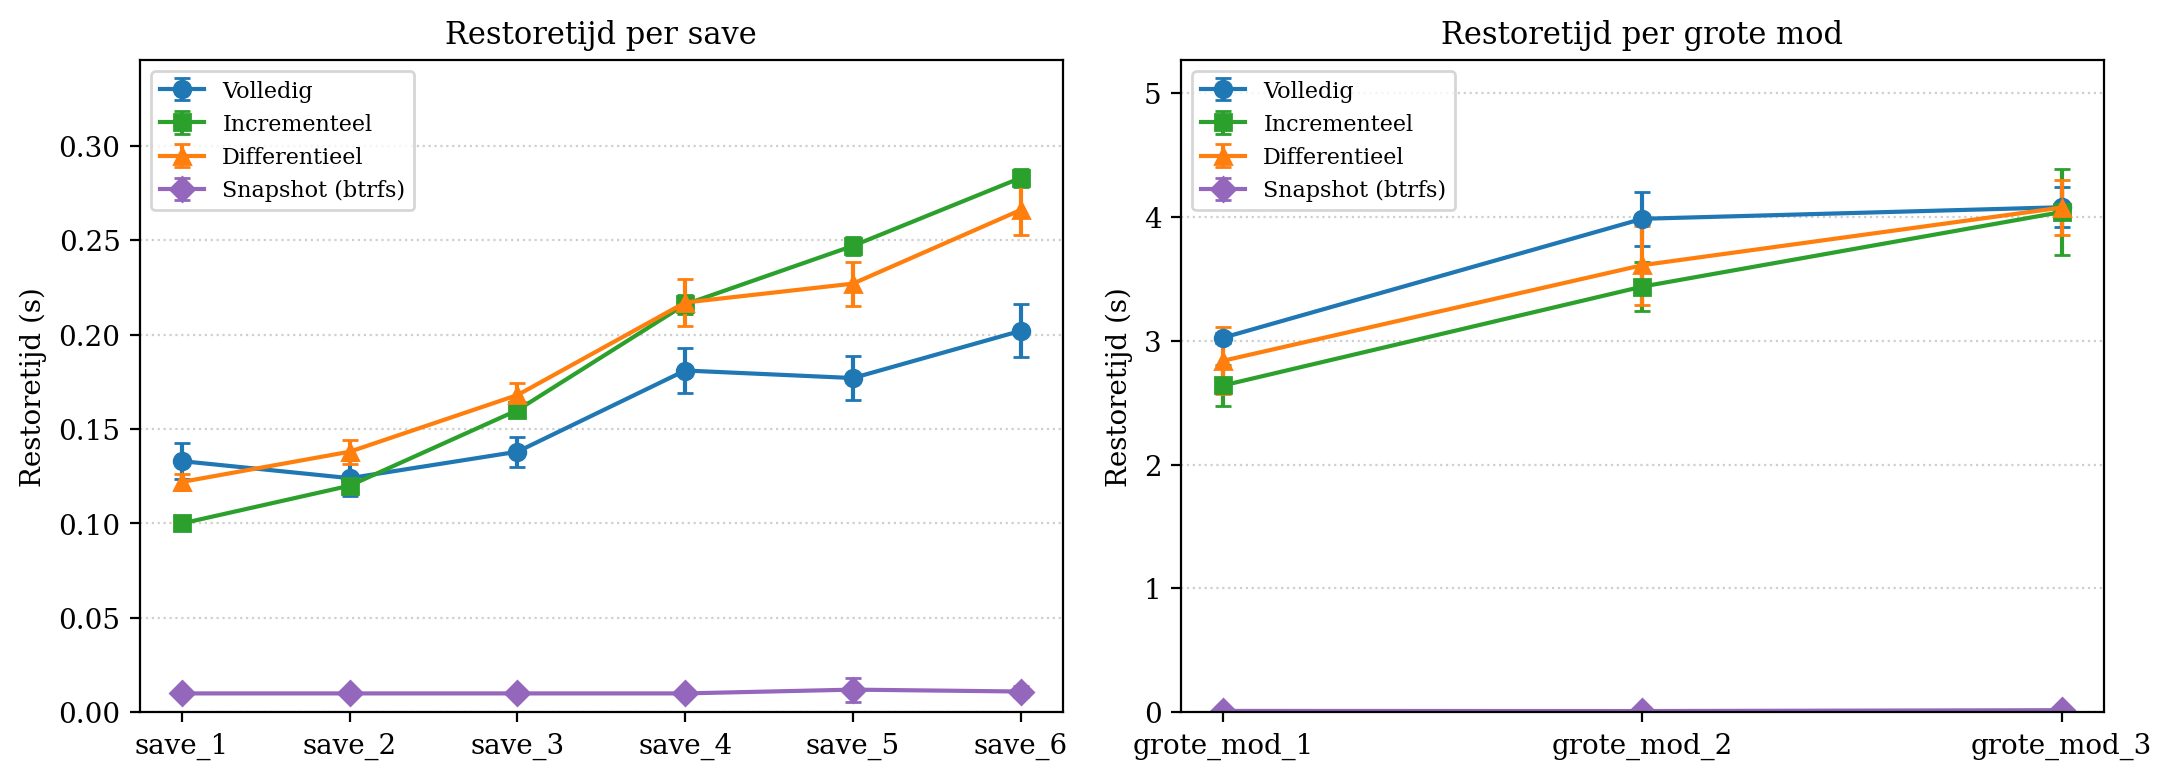
\includegraphics[width=\linewidth]{figures/fig_restore_time_per_point.png}
    \caption{Restoretijd per back-uppunt. De gerapporteerde tijd is de cumulatieve duur om alle archieven uit te pakken die nodig zijn om dat back-uppunt te herstellen.}
    \label{fig:restore-time}
\end{figure}

\paragraph{Volledige restore.}
Bij de saves stijgt de restoretijd geleidelijk van $\sim$0{,}13~s (\texttt{save\_1}) tot $\sim$0{,}20~s (\texttt{save\_6}), dit komt overeen met de groei van de archiefgrootte. Bij de mods zijn de restoretijden zeer gelijkaardig onder de verschillende methodes. Met \texttt{mod\_2} een verwaarloosbaar stuk langer dan incrementeel en differentieel rond $\sim$3{,}96~s.

\paragraph{Incrementele restore.}
De restoretijd stijgt zeer gelijmatig met elk back-uppunt, zowel bij saves ($\sim$0{,}10~s voor \texttt{save\_1} tot $\sim$0{,}28~s voor \texttt{save\_6}) als bij mods ($\sim$2{,}64~s voor \texttt{mod\_1} tot $\sim$4{,}04~s voor \texttt{mod\_3}). Dit lineaire verband is een direct gevolg van de cumulatieve aard van een incrementele restore: om \texttt{save\_6} terug te zetten moeten zes archieven sequentieel worden uitgepakt (basis + vijf incrementen), elk met zijn eigen overhead. Bij latere back-uppunten loopt deze opstartoverhead op en wordt de incrementele restore zelfs trager dan een volledige restore vanaf hetzelfde punt, bij de saves is dit duidelijk vanaf \texttt{save\_3}.

\paragraph{Differentiële restore.}
Differentieel bevindt zich tussen volledig en incrementeel. Het restoreproces vereist altijd exact twee archieven: de basis-back-up en de differentiële back-up van het gewenste punt. Daardoor is de opstartoverhead constant, maar de hoeveelheid uit te pakken data groeit mee met de grootte van het differentieel-archief. Voor de saves gedraagt de differentiële restore zich vrijwel identiek aan de incrementele ($\sim$0{,}12~s tot $\sim$0{,}27~s). bij de mods ligt \texttt{mod\_2} bij $\sim$3{,}61~s en \texttt{mod\_3} bij $\sim$4{,}07~s, ook gelijk aan incrementeel.

\paragraph{Snapshot-restore.}
Een snapshot-restore vergt in alle geteste configuraties slechts $\sim$10--17~ms, ongeacht de back-up. De operatie bestaat in essentie uit het hernoemen of swappen van het subvolume. Er moet dus geen data verplaatst worden. In een rollbackscenario is dit een groot verschil tegenover de tar-methodes: voor een mod-rollback is \texttt{btrfs} hier ruim 200 keer sneller dan de snelste tar-methode.

\subsection{CPU-gebruik tijdens de restore}
\label{subsec:restore-cpu}

Figuur~\ref{fig:restore-cpu} toont het CPU-gebruik per back-uppunt tijdens de restorefase.

\begin{figure}[h]
    \centering
    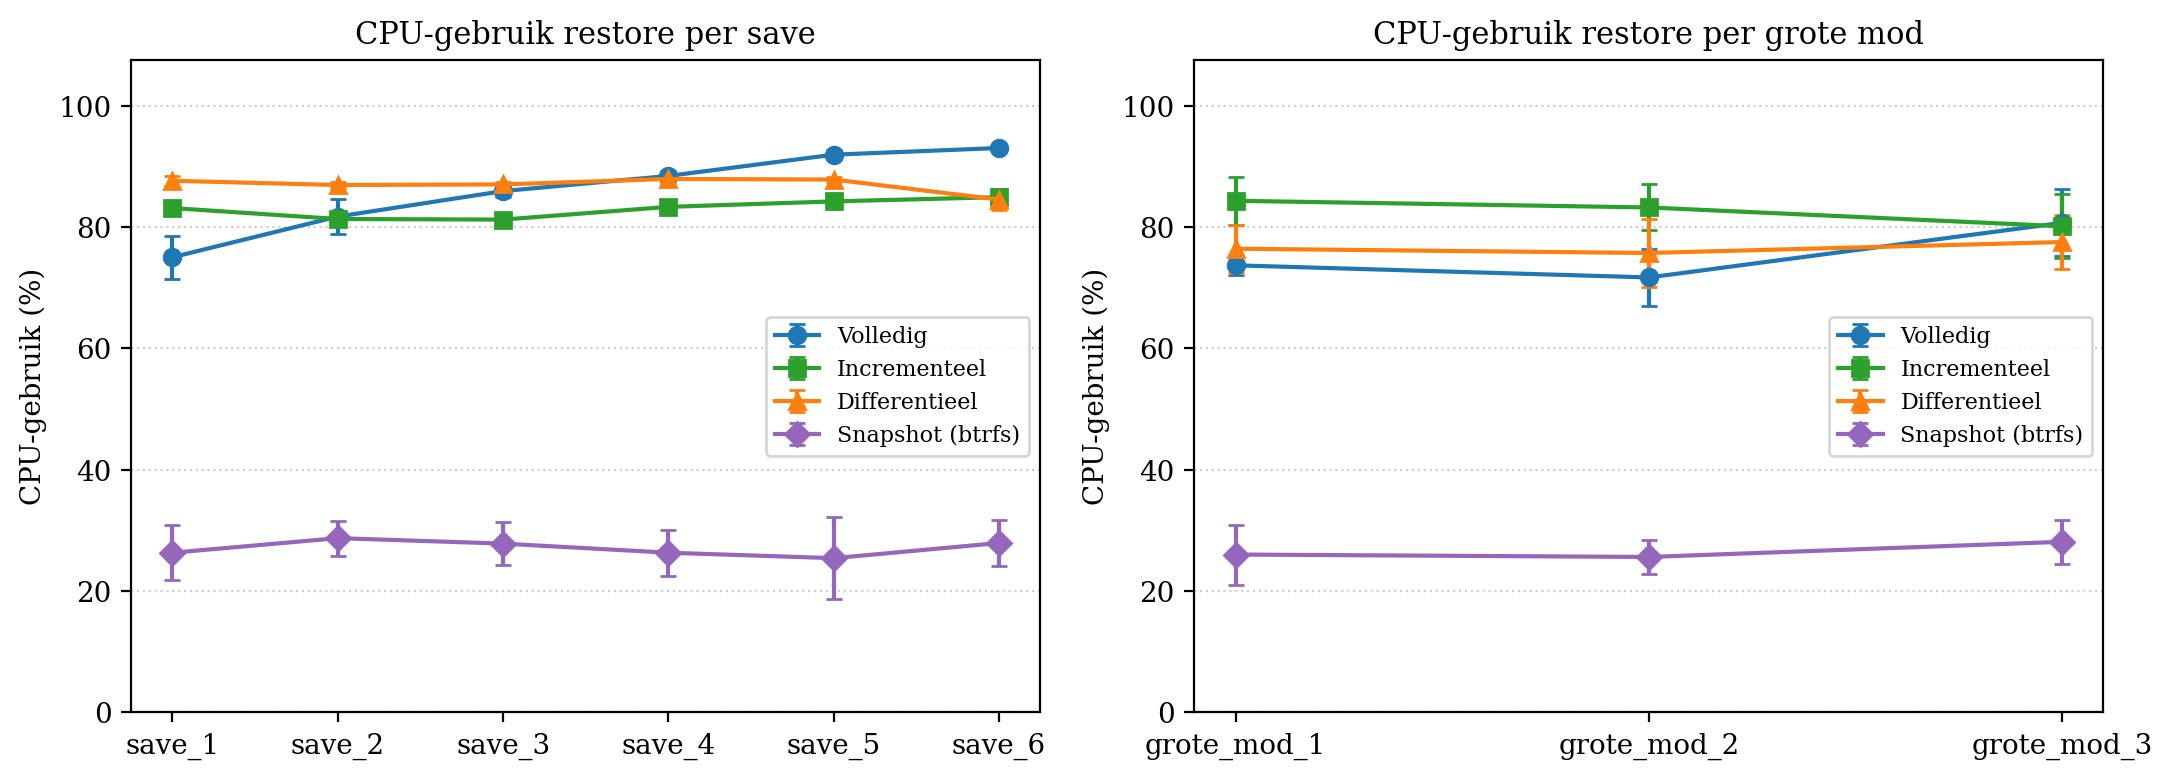
\includegraphics[width=\linewidth]{figures/fig_restore_cpu_per_point.png}
    \caption{CPU-gebruik tijdens de restorefase, per back-uppunt. De y-as is voor beide grafieken gelijk.}
    \label{fig:restore-cpu}
\end{figure}

Voor de tar-gebaseerde methodes ligt het CPU-gebruik tussen 75\% en 93\%, met de saves consistent hoger dan de mods. Dit toont aan dat het uitpakken van veel kleine bestanden CPU-intensiever is dan het uitpakken van weinig grote bestanden, wat overeenstemt met het idee dat de overhead per bestand (metadata-aanmaak, attribuut-toewijzing) zwaarder weegt naarmate er meer bestanden zijn. Bij de volledige restore van de saves stijgt het CPU-gebruik licht met elke back-up (van 75\% bij \texttt{save\_1} tot 93\% bij \texttt{save\_6}), wat overeenkomt met de groei van het archief en de toename van het aantal te schrijven bestanden.

De snapshot-restore blijft, net als bij de back-up, op $\sim$25--28\% en illustreert opnieuw dat het hier in gewoon om een metadata-operatie gaat.


\section{Synthese en conclusie}
\label{sec:synthese}

\subsection{Samenvattende vergelijking}

Tabel~\ref{tab:summary} vat de belangrijkste meetwaarden samen, geaggregeerd over alle back-uppunten heen om een overzichtelijke totaalbeeld te geven. De cijfers in deze tabel zijn sommen over de volledige dataset (de zes saves of de drie mods).

\begin{table}[h]
    \centering
    \caption{Samenvattende vergelijking van back-upmethodes zonder compressie, geaggregeerd over de hele dataset. Tijden in seconden, opslag in MB}
    \label{tab:summary}
    \small
    \begin{tabular}{lrrrrrr}
        \toprule
        & \multicolumn{3}{c}{\textbf{Saves (6 stuks, $\sim$0{,}6~GB)}}
        & \multicolumn{3}{c}{\textbf{Mods (3 stuks, $\sim$6{,}5~GB)}} \\
        \cmidrule(lr){2-4}\cmidrule(lr){5-7}
        \textbf{Methode} & Back-up & Restore & Opslag
        & Back-up & Restore & Opslag \\
        \midrule
        Volledig       & 0{,}80 & 0{,}96 &  630 &  9{,}48 & 11{,}05 & 6800 \\
        Incrementeel   & 0{,}24 & 1{,}13 &  196 &  4{,}06 & 10{,}11 & 2684 \\
        Differentieel  & 0{,}35 & 1{,}14 &  307 &  5{,}48 & 10{,}52 & 3221 \\
        Snapshot       & 0{,}33 & 0{,}06 &  112$^{\ast}$ & 1{,}85 & 0{,}04  & 2070$^{\ast}$ \\
        \bottomrule
    \end{tabular}
    
    \vspace{0.4em}
    \footnotesize $^{\ast}$ Voor de snapshotmethode betreft de vermelde opslag de \emph{totale fysieke voetafdruk} van de volledige snapshot-set, inclusief de gedeelde blokken die fysiek slechts één keer worden bewaard.
\end{table}

\subsection{Per-back-up observaties}

De analyse per back-uppunt brengt een aantal patronen aan het licht die in een gesommeerde voorstelling onzichtbaar zouden blijven:

\begin{itemize}
    \item \textbf{Het ``gratis'' tweede back-uppunt bij incrementeel.} Bij zowel saves als mods is het tweede back-uppunt extreem goedkoop in zowel tijd als opslag (\texttt{save\_2}: $\sim$14~ms en 9~MB; \texttt{mod\_2}: $\sim$0{,}88~s en 537~MB). Voor scenario's waarin een gebruiker zeer frequent kleine wijzigingen wenst vast te leggen, levert de incrementele methode een zeer gunstige verhouding op tussen werk en opslagvoetafdruk.
    \item \textbf{Cumulatieve groei van differentiële archieven.} Het verschil tussen incrementeel en differentieel komt pas vanaf het derde back-uppunt aan het licht en groeit daarna geleidelijk. \texttt{mod\_3} differentieel is bijvoorbeeld 2{,}5 keer zo groot als het corresponderende increment. Voor lange reeksen back-uppunten weegt deze cumulatieve groei zwaar door op de totale opslagkost.
    \item \textbf{Cumulatieve groei van incrementele restoretijd.} Hoewel een incrementele back-up zelf goedkoop is, vereist het herstellen ervan het sequentieel uitpakken van alle voorafgaande archieven. Bij de saves wordt incrementele restore vanaf \texttt{save\_4} zelfs trager dan een volledige restore vanaf hetzelfde punt. Dit is een belangrijke afweging: een incrementele strategie minimaliseert het werk per back-up, ten koste van het werk per restore.
    \item \textbf{Voorspelbaarheid van snapshots.} De snapshotmethode vertoont in alle metrieken een constante kost per back-uppunt. Dit staat in scherp contrast met de tar-methodes, waar de individuele kost sterk varieert afhankelijk van de back-up en de tussentijdse wijzigingen. Voor een back-upsysteem dat geautomatiseerd wordt (bijvoorbeeld bij elke mod-update) is voorspelbare kost een belangrijke eigenschap.
    \item \textbf{Blokniveau-deduplicatie van btrfs.} Voor de drie mods samen bedraagt de fysieke voetafdruk van de snapshot-set $\sim$2{,}07~GB, terwijl de incrementele tar-strategie $\sim$2{,}68~GB nodig heeft. Btrfs slaagt erin op blokniveau efficiënter te dedupliceren dan tar op bestandsniveau, zelfs zonder dat er compressie wordt toegepast. Bij de saves is het verschil nog uitgesprokener ($\sim$112~MB tegenover $\sim$196~MB).
\end{itemize}

\subsection{Aanbeveling voor savegames}

Savegames worden frequent overschreven, zijn relatief klein en moeten snel kunnen worden teruggezet. Op basis van de per-back-up analyse:

\begin{itemize}
    \item Op deze schaal zijn alle back-upmethodes sub-seconde per back-up. De keuze wordt daardoor niet bepaald door de back-upsnelheid alleen.
    \item De restoretijd vertoont \emph{wel} een methode-afhankelijk verschil dat oploopt met de back-uppunten. Voor recente back-uppunten (\texttt{save\_5} of \texttt{save\_6}) is een volledige restore sneller dan een incrementele of differentiële restore. Een snapshot-restore is op alle punten ongeveer twintig keer sneller dan welke tar-methode ook.
    \item Het opslagverbruik is in absolute zin verwaarloosbaar (honderden MB op moderne SSDs). Het kleine opslagvoordeel van incrementeel of snapshot weegt hier niet zwaar door.
\end{itemize}

De snapshotmethode is het aantrekkelijkst voor savegames: de constante back-upkost per punt, quasi-instantane rollbacks en een minimale fysieke voetafdruk dankzij copy-on-write. Het belangrijkste nadeel is de afhankelijkheid van btrfs als bestandssysteem. Voor opstellingen waar btrfs niet beschikbaar is, vormt de \emph{incrementele} methode een goed alternatief: de back-uptijd per punt is laag (vaak onder de 50~ms), het opslaggebruik is het zuinigst, en de oplopende restoretijd blijft binnen aanvaardbare grenzen voor savegames van deze omvang. Een volledige back-upstrategie heeft hier geen functioneel voordeel en kost meer ruimte.

\subsection{Aanbeveling voor grote mods}

Voor grote mods is de keuze duidelijker:

\begin{itemize}
    \item De volledige methode is in alle dimensies inferieur. Elke back-up duurt $\sim$3~s en kost $\sim$2~GB aan opslag, ongeacht hoeveel of hoe weinig de mod tussen versies wijzigt. De methode benut bovendien ook geen enkele optimalisatie.
    \item De incrementele methode profiteert sterk van het feit dat opeenvolgende mod-versies veel data delen. \texttt{mod\_3} wordt incrementeel weggeschreven in $\sim$0{,}54~s en kost slechts $\sim$358~MB. Het nadeel is dat een rollback naar een recent punt het sequentieel uitpakken van alle voorgaande versies vereist, met restoretijden die oplopen tot $\sim$4~s.
    \item De differentiële methode biedt geen voordeel ten opzichte van de incrementele. De back-upsnelheid is slechter (meer data per back-up), het opslaggebruik is hoger, en de restoretijd is vergelijkbaar.
    \item De snapshotmethode is opnieuw superieur. Een back-up van een 2{,}5~GB-mod kost $\sim$0{,}6~s en een rollback gebeurt in minder dan 20~ms. De fysieke opslagvoetafdruk voor de drie mod-versies samen ligt bovendien onder die van de incrementele tar-strategie.
\end{itemize}

Voor mods is de winst van btrfs-snapshots zo groot dat dit als voorkeur\-strategie wordt aangenomen wanneer het bestandssysteem ondersteund is. De snelheid van een snapshot-rollback maakt het bovendien mogelijk om \emph{voor elke mod-update} automatisch een back-up\-punt aan te maken, zonder dat de gebruiker een merkbare vertraging ondervindt. Indien btrfs niet beschikbaar is, vormt een incrementele tar-back-up het beste compromis: de eerste back-up duurt $\sim$2{,}6~s (volledig basisarchief), maar daaropvolgende incrementen zijn aanzienlijk lichter.

\section{Analyse van de compressie-algoritmes}
\label{sec:compressie}

\subsection{Doel en opzet van deze analyse}

In dit deel wordt onderzocht welk compressie-algoritme het meest geschikt is om gecombineerd te worden met de back-upmethodes uit de vorige sectie. Acht varianten werden getest: geen compressie als referentie, en zeven algoritmes die rechtstreeks via de \texttt{tar}-command beschikbaar zijn (\texttt{gzip}, \texttt{bzip2}, \texttt{xz}, \texttt{lzma}, \texttt{lzip}, \texttt{lzop} en \texttt{zstd}). De algoritmes zijn te groeperen in vijf families:

\begin{itemize}
    \item \textbf{DEFLATE} -- \texttt{gzip}: het oudste en meest verspreide algoritme, gebaseerd op LZ77 + Huffman-codering.
    \item \textbf{BWT} -- \texttt{bzip2}: gebruikt de Burrows-Wheeler-transformatie en biedt een betere compressieratio dan gzip, maar is aanzienlijk trager.
    \item \textbf{LZMA-familie} -- \texttt{xz}, \texttt{lzma}, \texttt{lzip}: drie containers rond hetzelfde LZMA/LZMA2-algoritme, dat een zeer hoge compressieratio levert ten koste van substantiële rekentijd en geheugen. Van deze drie ondersteunt \texttt{xz} multithreading.
    \item \textbf{LZ-snel} -- \texttt{lzop}: een variant van LZ77 die is ontworpen voor maximale snelheid, ten koste van een relatief zwakke compressieratio.
    \item \textbf{Modern} -- \texttt{zstd} (Zstandard, ontwikkeld door Facebook): combineert een snelle LZ77-variant met een entropie- codering (FSE/Huffman) en biedt op het standaardniveau een goede verhouding tussen snelheid en compressieratio. Ondersteunt ook multithreading.
\end{itemize}

Ondanks de keuze die reeds in sectie~\ref{sec:results-backup} werd besproken, beperkt deze analyse zich tot toepassing op de \textbf{volledige} back-upmethode. Deze methode levert per back-up de meeste data om te comprimeren en biedt zo het zuiverste beeld van de inherente eigenschappen van elk algoritme. De bevindingen blijven grotendeels overdraagbaar naar de incrementele en differentiële methode, omdat de compressie-eigenschappen (ratio, doorvoer, geheugen) onafhankelijk zijn van de specifieke samenstelling van het te comprimeren tar-archief.

In tegenstelling tot de vorige sectie worden de metrieken hier gerapporteerd als \emph{totaal over de hele dataset}: de zes saves of de drie mods samen. Dit aggregatieniveau volstaat om de algoritmes onderling te vergelijken; de individuele variatie tussen back-uppunten werd reeds in sectie~\ref{sec:results-backup} besproken en wordt door de keuze van compressie-algoritme niet merkelijk veranderd.

\subsection{Compressieratio en archiefgrootte}
\label{subsec:compressie-ratio}

Figuur~\ref{fig:compression-size} toont de archiefgrootte per algoritme voor beide datasets, met de oorspronkelijke datasetgrootte als referentie in de titel.

\begin{figure}[h]
    \centering
    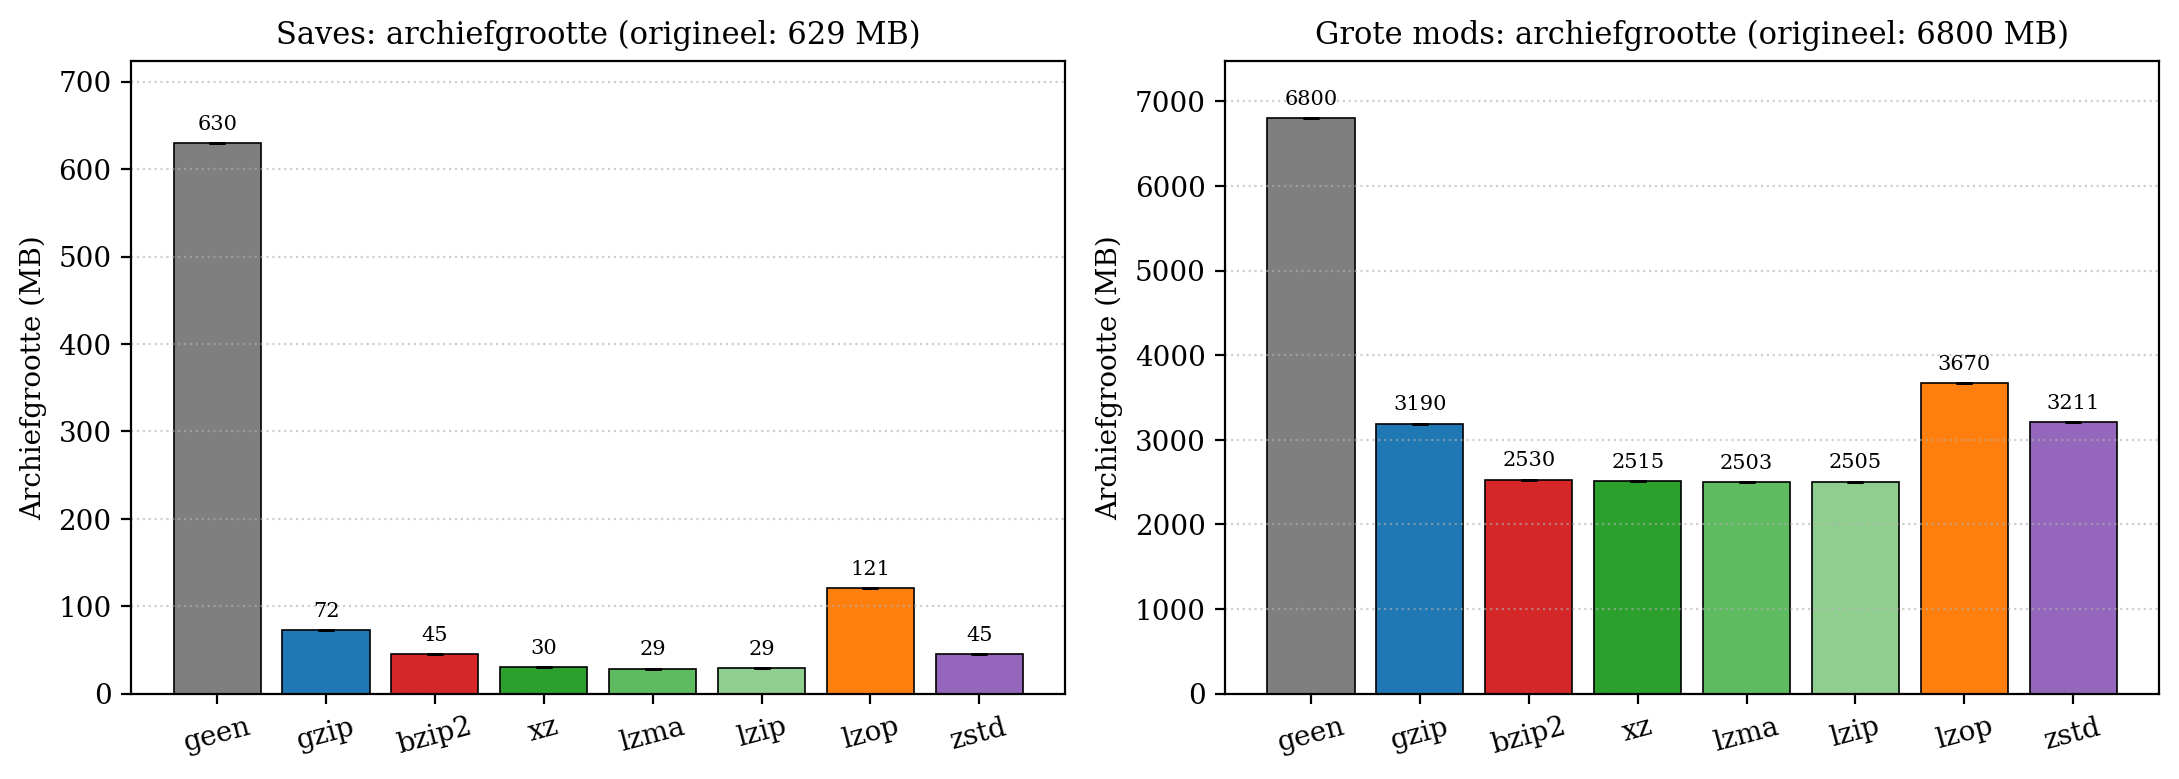
\includegraphics[width=\linewidth]{figures/fig_compression_size.png}
    \caption{Archiefgrootte per algoritme, voor de volledige back-up van respectievelijk de zes saves (links) en de drie mods (rechts). De ongecomprimeerde variant geldt als referentie.}
    \label{fig:compression-size}
\end{figure}

\paragraph{Saves.}
De zes savegames samen ($\sim$629~MB origineel) laten zich extreem goed comprimeren. \texttt{gzip} reduceert het archief tot $\sim$72~MB (ratio 0{,}115); de LZMA-familie haalt nog meer winst en duwt de archiefgrootte tot onder de 30~MB (ratio $\sim$0{,}046 -- 0{,}048). De spreiding tussen \texttt{xz}, \texttt{lzma} en \texttt{lzip} is verwaarloosbaar, ze gebruiken intern hetzelfde algoritme. Aan de andere kant van het spectrum staat \texttt{lzop}, dat slechts tot $\sim$121~MB inkort (ratio 0{,}192). \texttt{zstd} en \texttt{bzip2} landen beide rond $\sim$45~MB (ratio 0{,}072). Dat savegames zo sterk comprimeren wijst erop dat ze grotendeels uit gestructureerde tekstdata bestaan, met veel herhaling.

\paragraph{Mods.}
Bij de mods is het beeld dramatisch anders. Alle algoritmes convergeren rond een ratio van 0{,}37 -- 0{,}54, en het verschil tussen het beste algoritme (\texttt{lzma}, $\sim$2503~MB) en het slechtste (\texttt{lzop}, $\sim$3670~MB) is slechts een factor 1{,}5. \texttt{gzip}, \texttt{zstd} en \texttt{lzop} blijven steken rond $\sim$3200 -- 3670~MB. Voor de mod-werklast levert de keuze van het algoritme dus voornamelijk een afweging op tussen compressietijd en geheugengebruik, niet zozeer een verschil in eindgrootte.

\subsection{Compressie- en decompressietijd}
\label{subsec:compressie-tijd}

Figuur~\ref{fig:compression-time} toont de back-up- en restoretijd per algoritme. Wegens het zeer brede bereik wordt een logaritmische y-as gebruikt.

\begin{figure}[h]
    \centering
    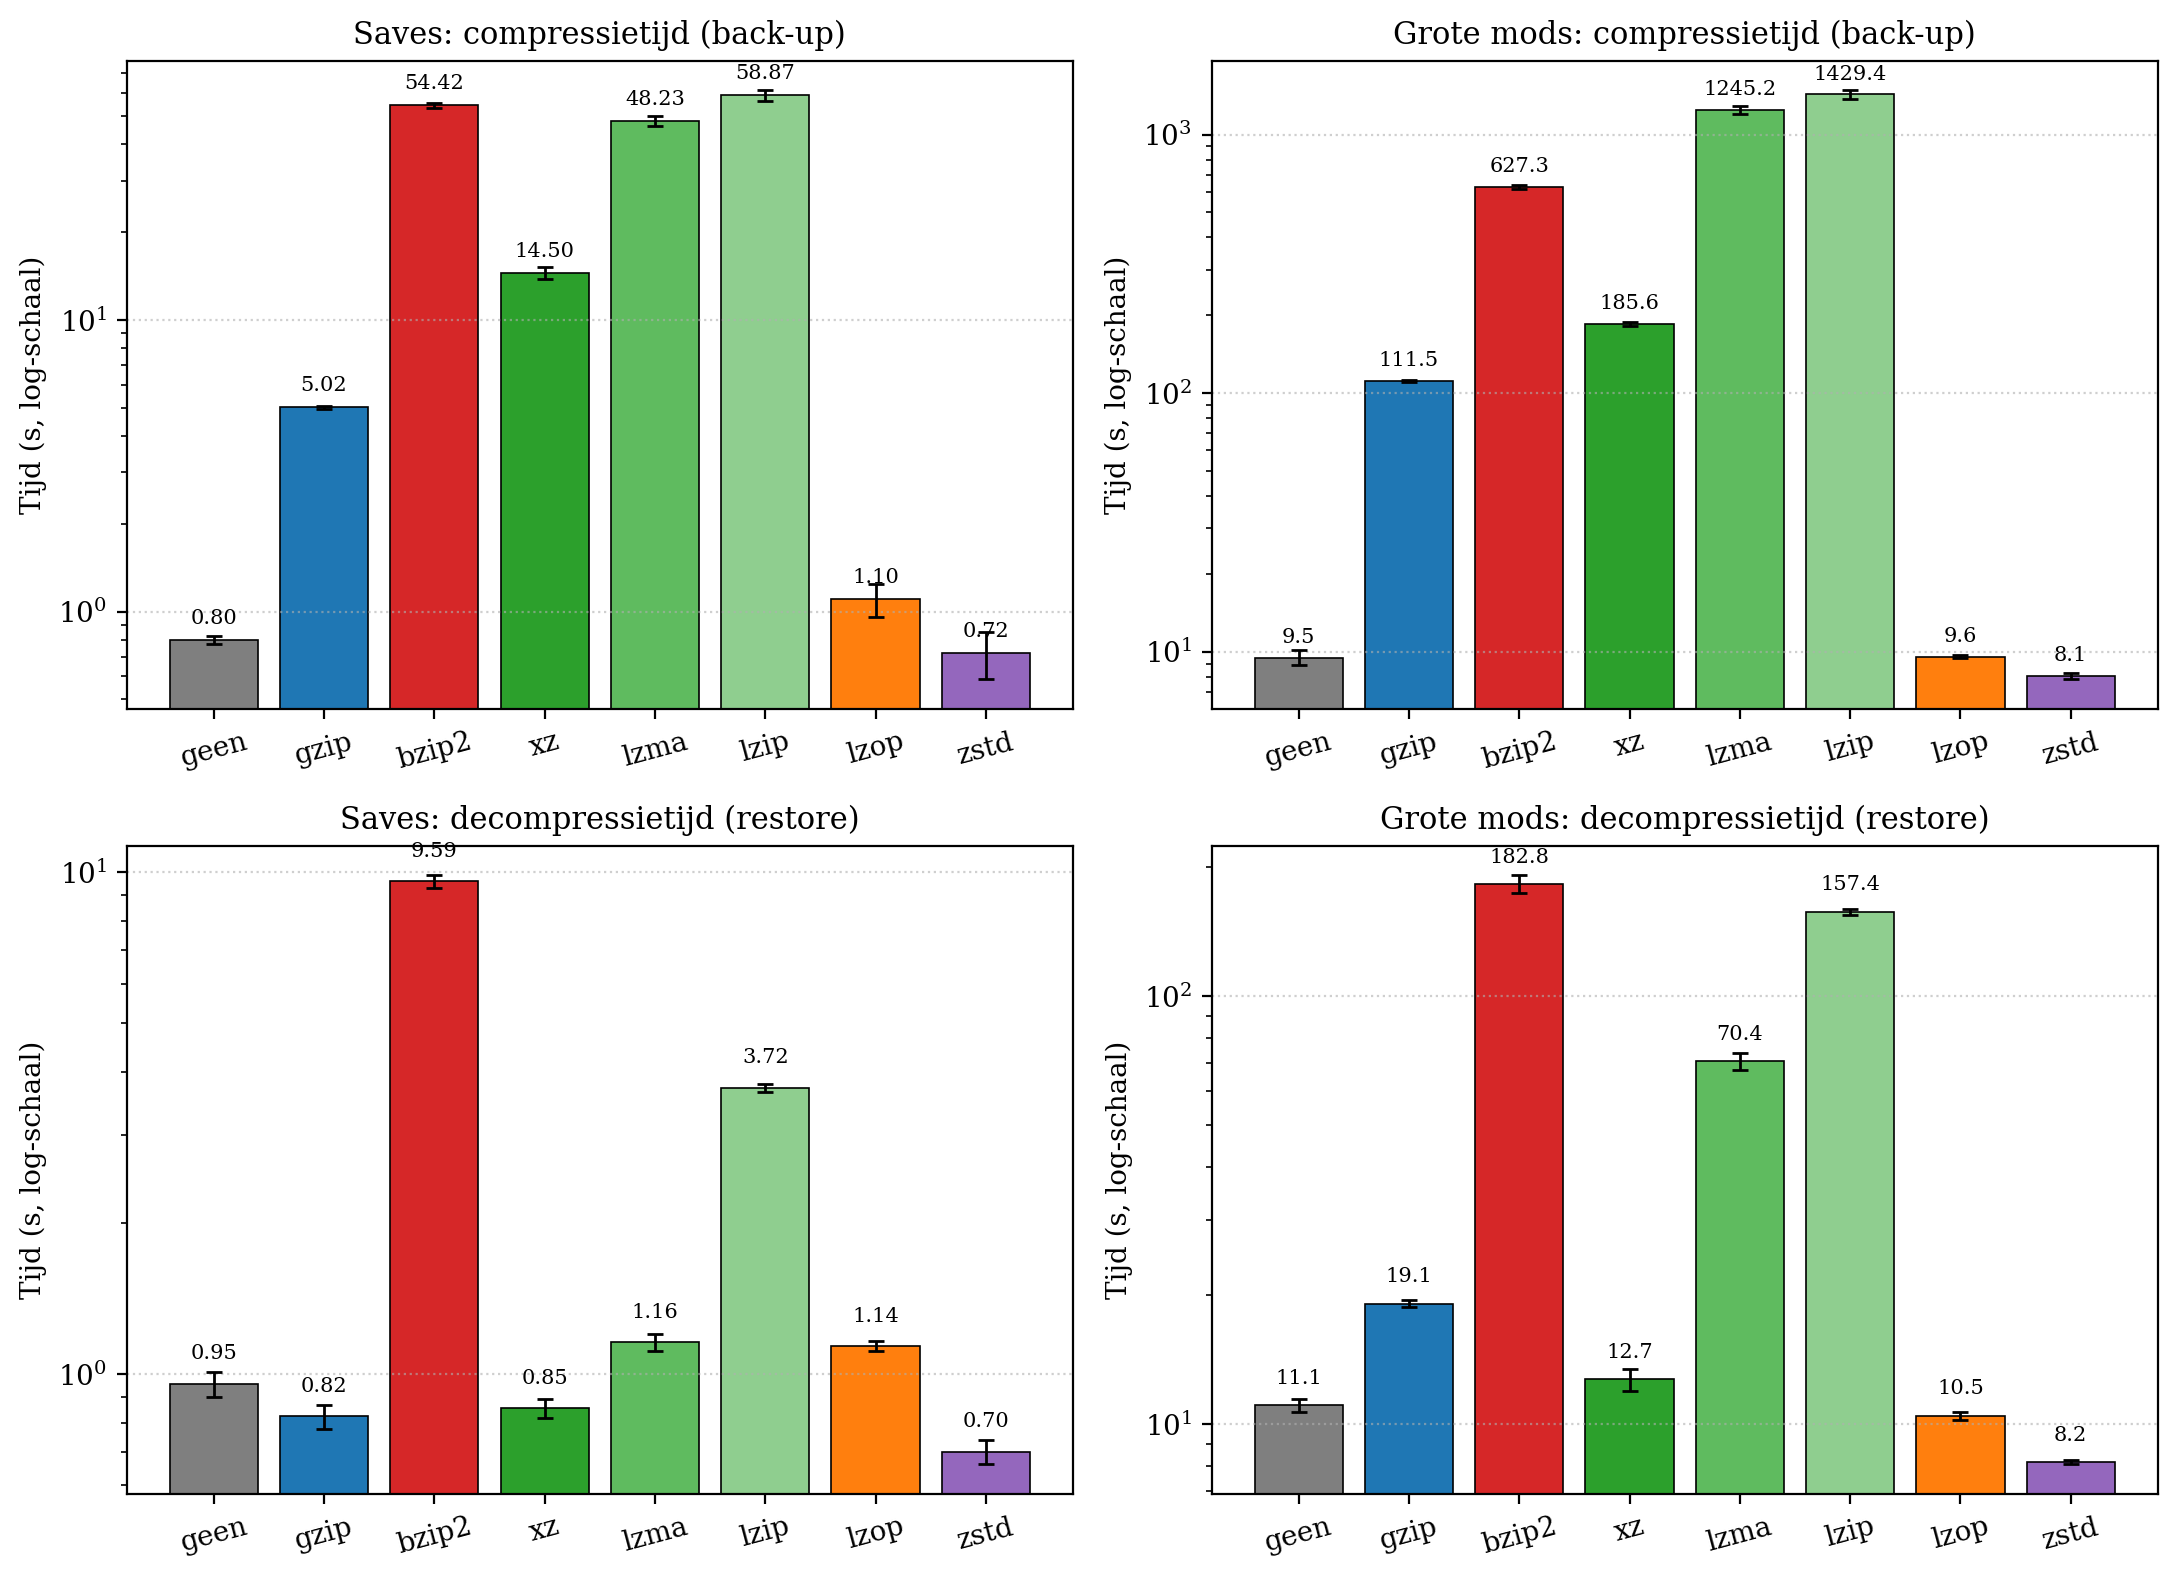
\includegraphics[width=\linewidth]{figures/fig_compression_time.png}
    \caption{Compressietijd (boven) en decompressietijd (onder) per algoritme, voor saves (links) en mods (rechts). De y-as is logaritmisch wegens het grote bereik. Foutbalken: standaardafwijking over 10 runs.}
    \label{fig:compression-time}
\end{figure}

\paragraph{Compressietijd (back-up).}
Voor de mods spreidt de compressietijd zich uit over drie orden van grootte: \texttt{zstd} en \texttt{lzop} blijven onder de 10 seconden, \texttt{gzip} doet er $\sim$112~s over, \texttt{xz} $\sim$186~s, \texttt{bzip2} $\sim$627~s, en \texttt{lzma}/\texttt{lzip} respectievelijk $\sim$1245~s en $\sim$1429~s. Dat een back-up van 6{,}5~GB met \texttt{lzip} bijna 24 minuten duurt, is voor een interactief back-upsysteem onaanvaardbaar. \texttt{zstd} is bovendien zelfs \emph{sneller} dan de ongecomprimeerde tar-back-up ($\sim$8{,}1~s tegenover $\sim$9{,}5~s). Dit is geen meetfout: \texttt{zstd} draait parallel over meerdere threads (zie sectie~\ref{subsec:compressie-cpu}) en compenseert de extra rekentijd door de I/O-belasting te verminderen, een gecomprimeerd archief is kleiner en hoeft minder bytes naar de SSD te schrijven.

Voor de saves geldt dezelfde rangorde, maar op een andere absolute schaal. \texttt{zstd} en \texttt{lzop} blijven onder 1{,}1~s, \texttt{gzip} doet er $\sim$5~s over, en de zware algoritmes (\texttt{bzip2}, \texttt{lzma}, \texttt{lzip}) zitten bij 48 -- 59~s. \texttt{xz} valt op met $\sim$14{,}5~s; opnieuw te verklaren door multithreading.

\paragraph{Decompressietijd (restore).}
Het beeld bij decompressie is fundamenteel anders. \texttt{zstd} ($\sim$8{,}2~s op mods, $\sim$0{,}70~s op saves) en \texttt{xz} zijn de snelste decompressors. \texttt{xz} ondersteunt namelijk parallelle decompressie, en presteert daarom drastisch beter dan zijn single-threaded familieleden \texttt{lzma} en \texttt{lzip}. \texttt{lzma} doet er $\sim$70~s over op de mods (factor 5{,}5 trager dan xz); \texttt{lzip} zelfs $\sim$157~s. \texttt{bzip2} is bij decompressie nog trager dan bij compressie ten opzichte van de LZMA-familie. Waar gzip en zstd typisch veel sneller decomprimeren dan comprimeren, blijft de decompressie van bzip2 relatief duur ($\sim$183~s op de mods). \texttt{lzop} is consistent snel maar wint hier geen significant voordeel ten opzichte van \texttt{zstd} of \texttt{xz}.

Voor een back-upsysteem dat in een rollbackscenario gebruikt zal worden, is de decompressietijd een zeer belangrijke factor. \texttt{lzip} en \texttt{bzip2} sluiten zichzelf hiermee effectief uit voor grote datasets: een restoreoperatie van enkele minuten op een mod-update van enkele gigabytes vraagt een extreem lange wachttijd op het kritieke moment waarop de gebruiker juist snel wil terugkeren.

\subsection{CPU-gebruik}
\label{subsec:compressie-cpu}

Figuur~\ref{fig:compression-cpu} toont het CPU-gebruik tijdens compressie en decompressie.

\begin{figure}[h]
    \centering
    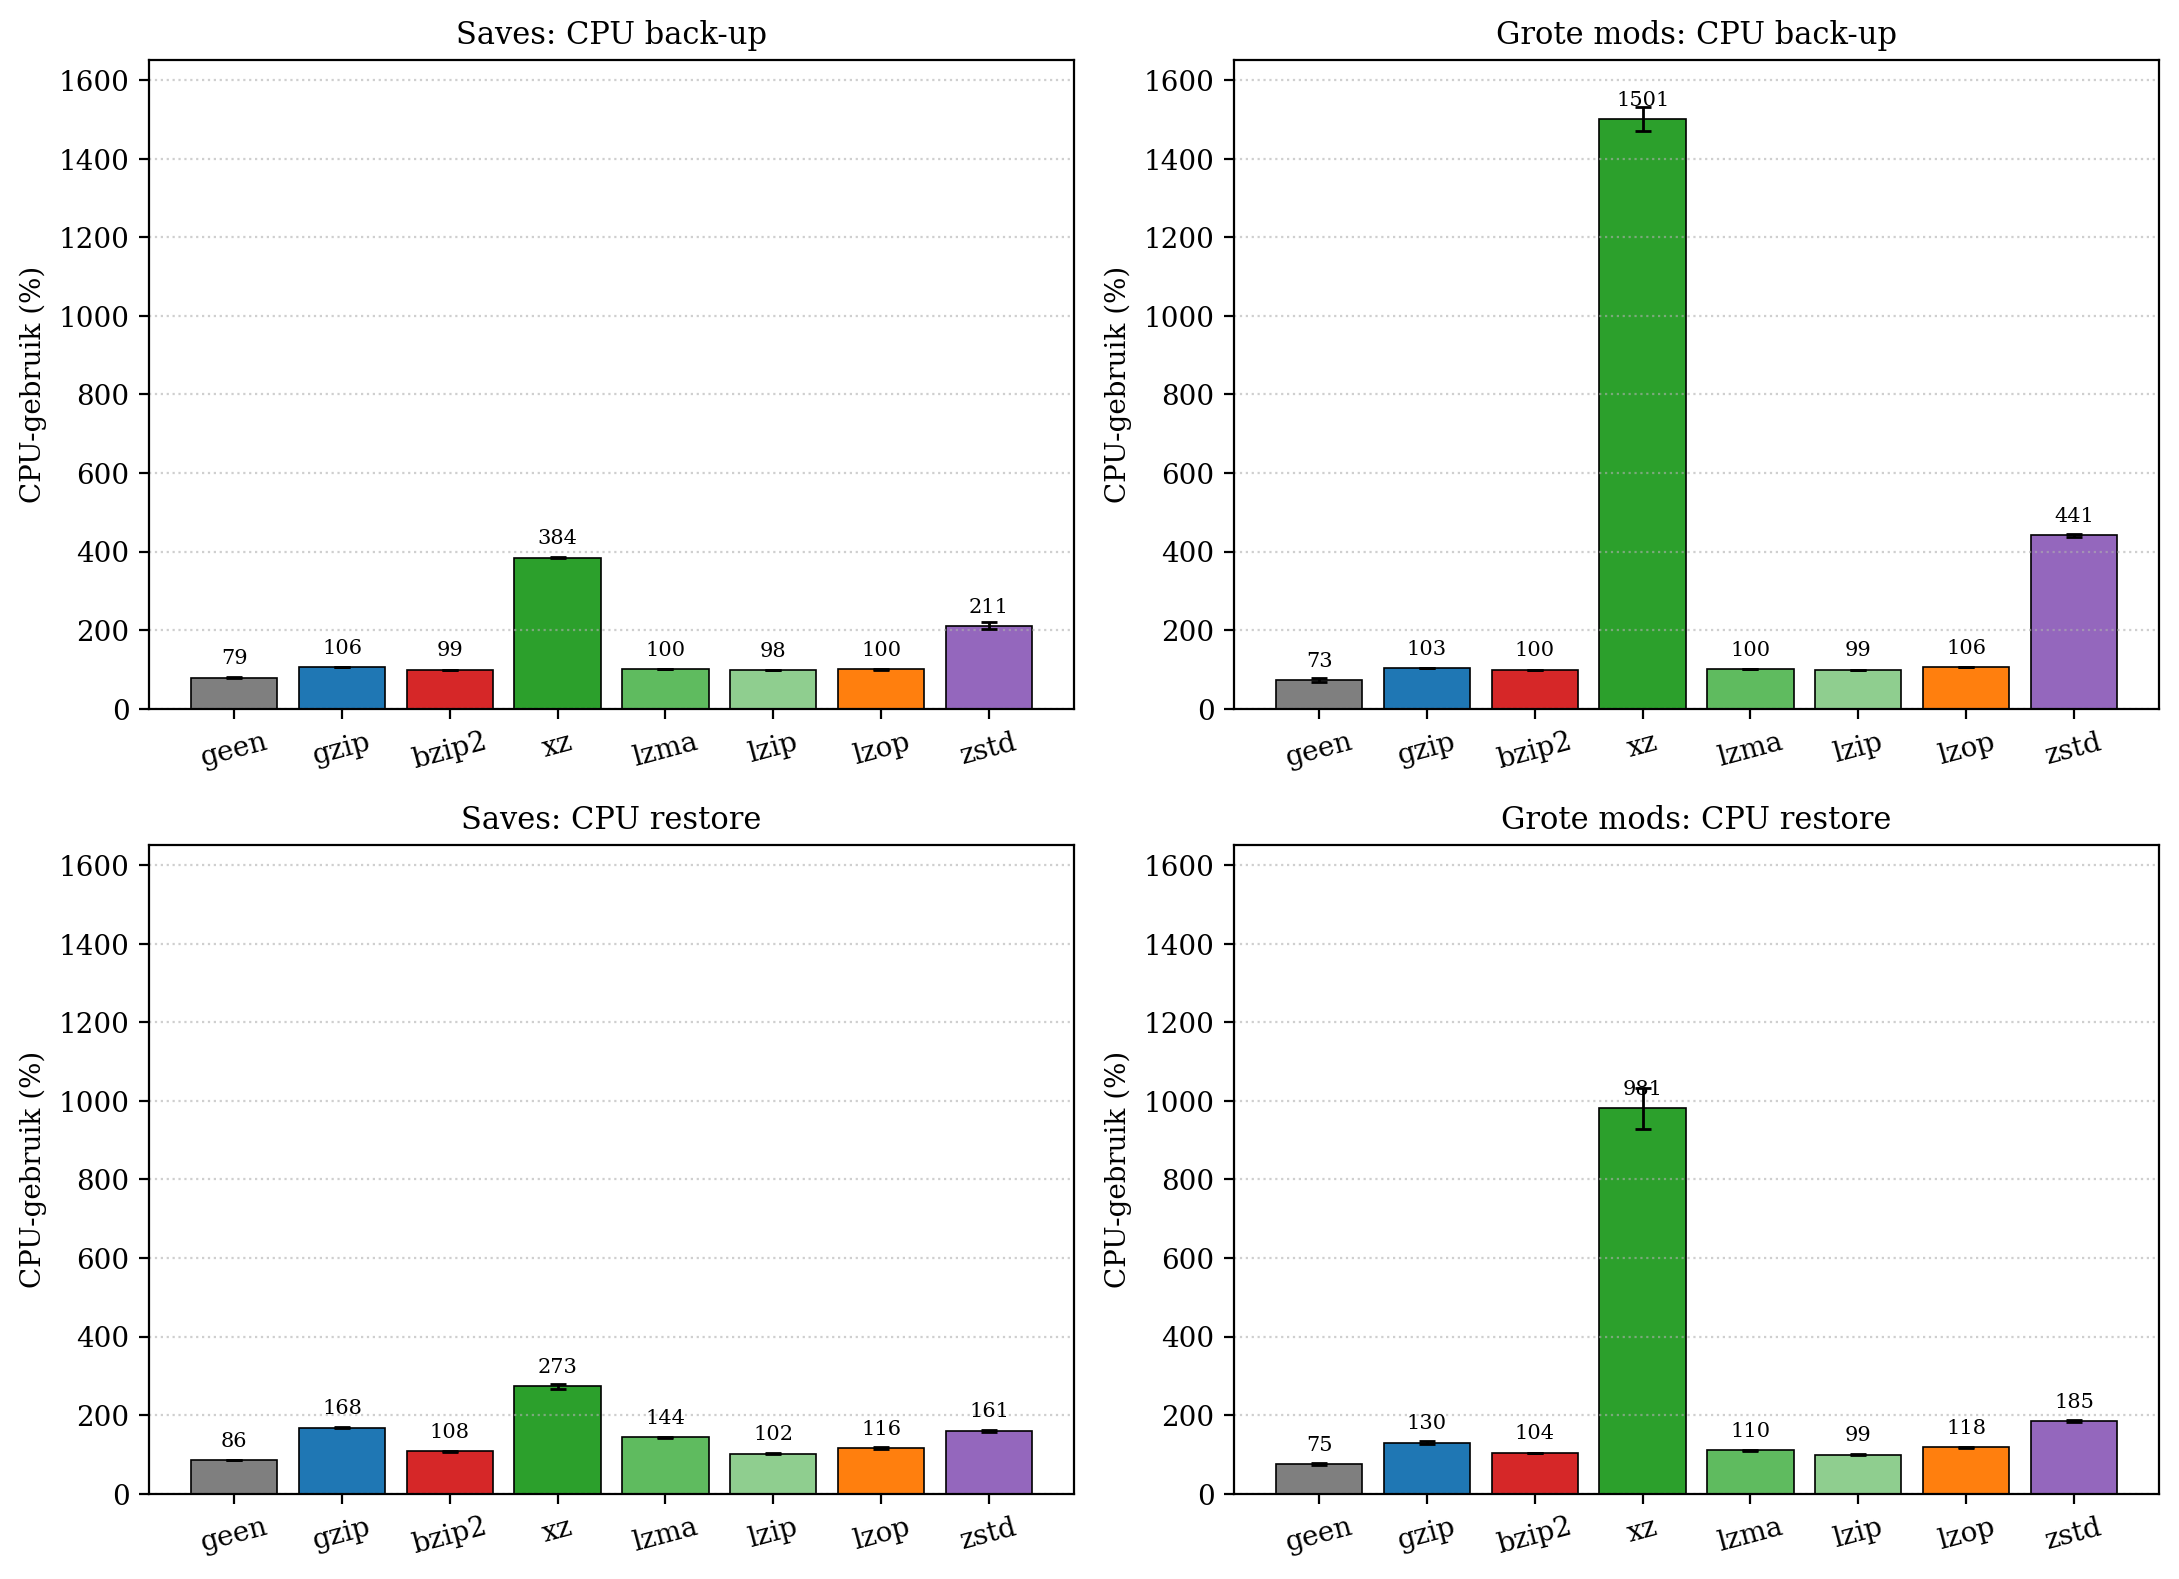
\includegraphics[width=\linewidth]{figures/fig_compression_cpu.png}
    \caption{CPU-gebruik per algoritme. De y-as is voor alle vier de panelen gelijk. Een waarde van 100\% komt overeen met één volledige thread; het maximum op deze 16-thread-CPU is 1600\%.}
    \label{fig:compression-cpu}
\end{figure}

\paragraph{Single-threaded versus multi-threaded.}
Het meest opvallende patroon is de scheiding tussen single-threaded algoritmes (\texttt{gzip}, \texttt{bzip2}, \texttt{lzma}, \texttt{lzip}, \texttt{lzop}: telkens rond 100\%) en multi-threaded algoritmes (\texttt{xz}, \texttt{zstd}). Op de mods bereikt \texttt{xz} $\sim$1500\% -- bijna 15 threads vol -- en \texttt{zstd} $\sim$441\% ($\sim$4 -- 5 threads). Dit verklaart waarom deze twee algoritmes ondanks hun rekenintensiteit nog vlotte wandkloktijden halen.

Op de saves is het multithreading-voordeel beperkter omdat de afzonderlijke archieven (gemiddeld $\sim$100~MB) te klein zijn om de parallelle pipeline van \texttt{xz} volledig te benutten: de gemeten waarde zakt naar $\sim$385\%. Ook \texttt{zstd} schakelt op kleine inputs minder threads in.

\paragraph{Decompressie.}
Bij decompressie zijn dezelfde patronen zichtbaar. \texttt{xz} blijft de enige van de LZMA-familie die multithreaded decomprimeert. Bij \texttt{lzma} en \texttt{lzip} blijft het CPU-gebruik beperkt tot $\sim$100\%. \texttt{zstd} bereikt $\sim$185\% bij decompressie van de mods, wat overeenkomt met ongeveer twee threads. \texttt{gzip} gebruikt bij decompressie meer dan 100\% (130 -- 168\%). Dit komt doordat de \texttt{tar}-pipeline de uitpak-thread parallel laat lopen met de schrijf-thread.

\subsection{Geheugengebruik}
\label{subsec:compressie-mem}

Figuur~\ref{fig:compression-mem} toont het piek-RSS per algoritme. De y-as is logaritmisch wegens het zeer grote bereik.

\begin{figure}[h]
    \centering
    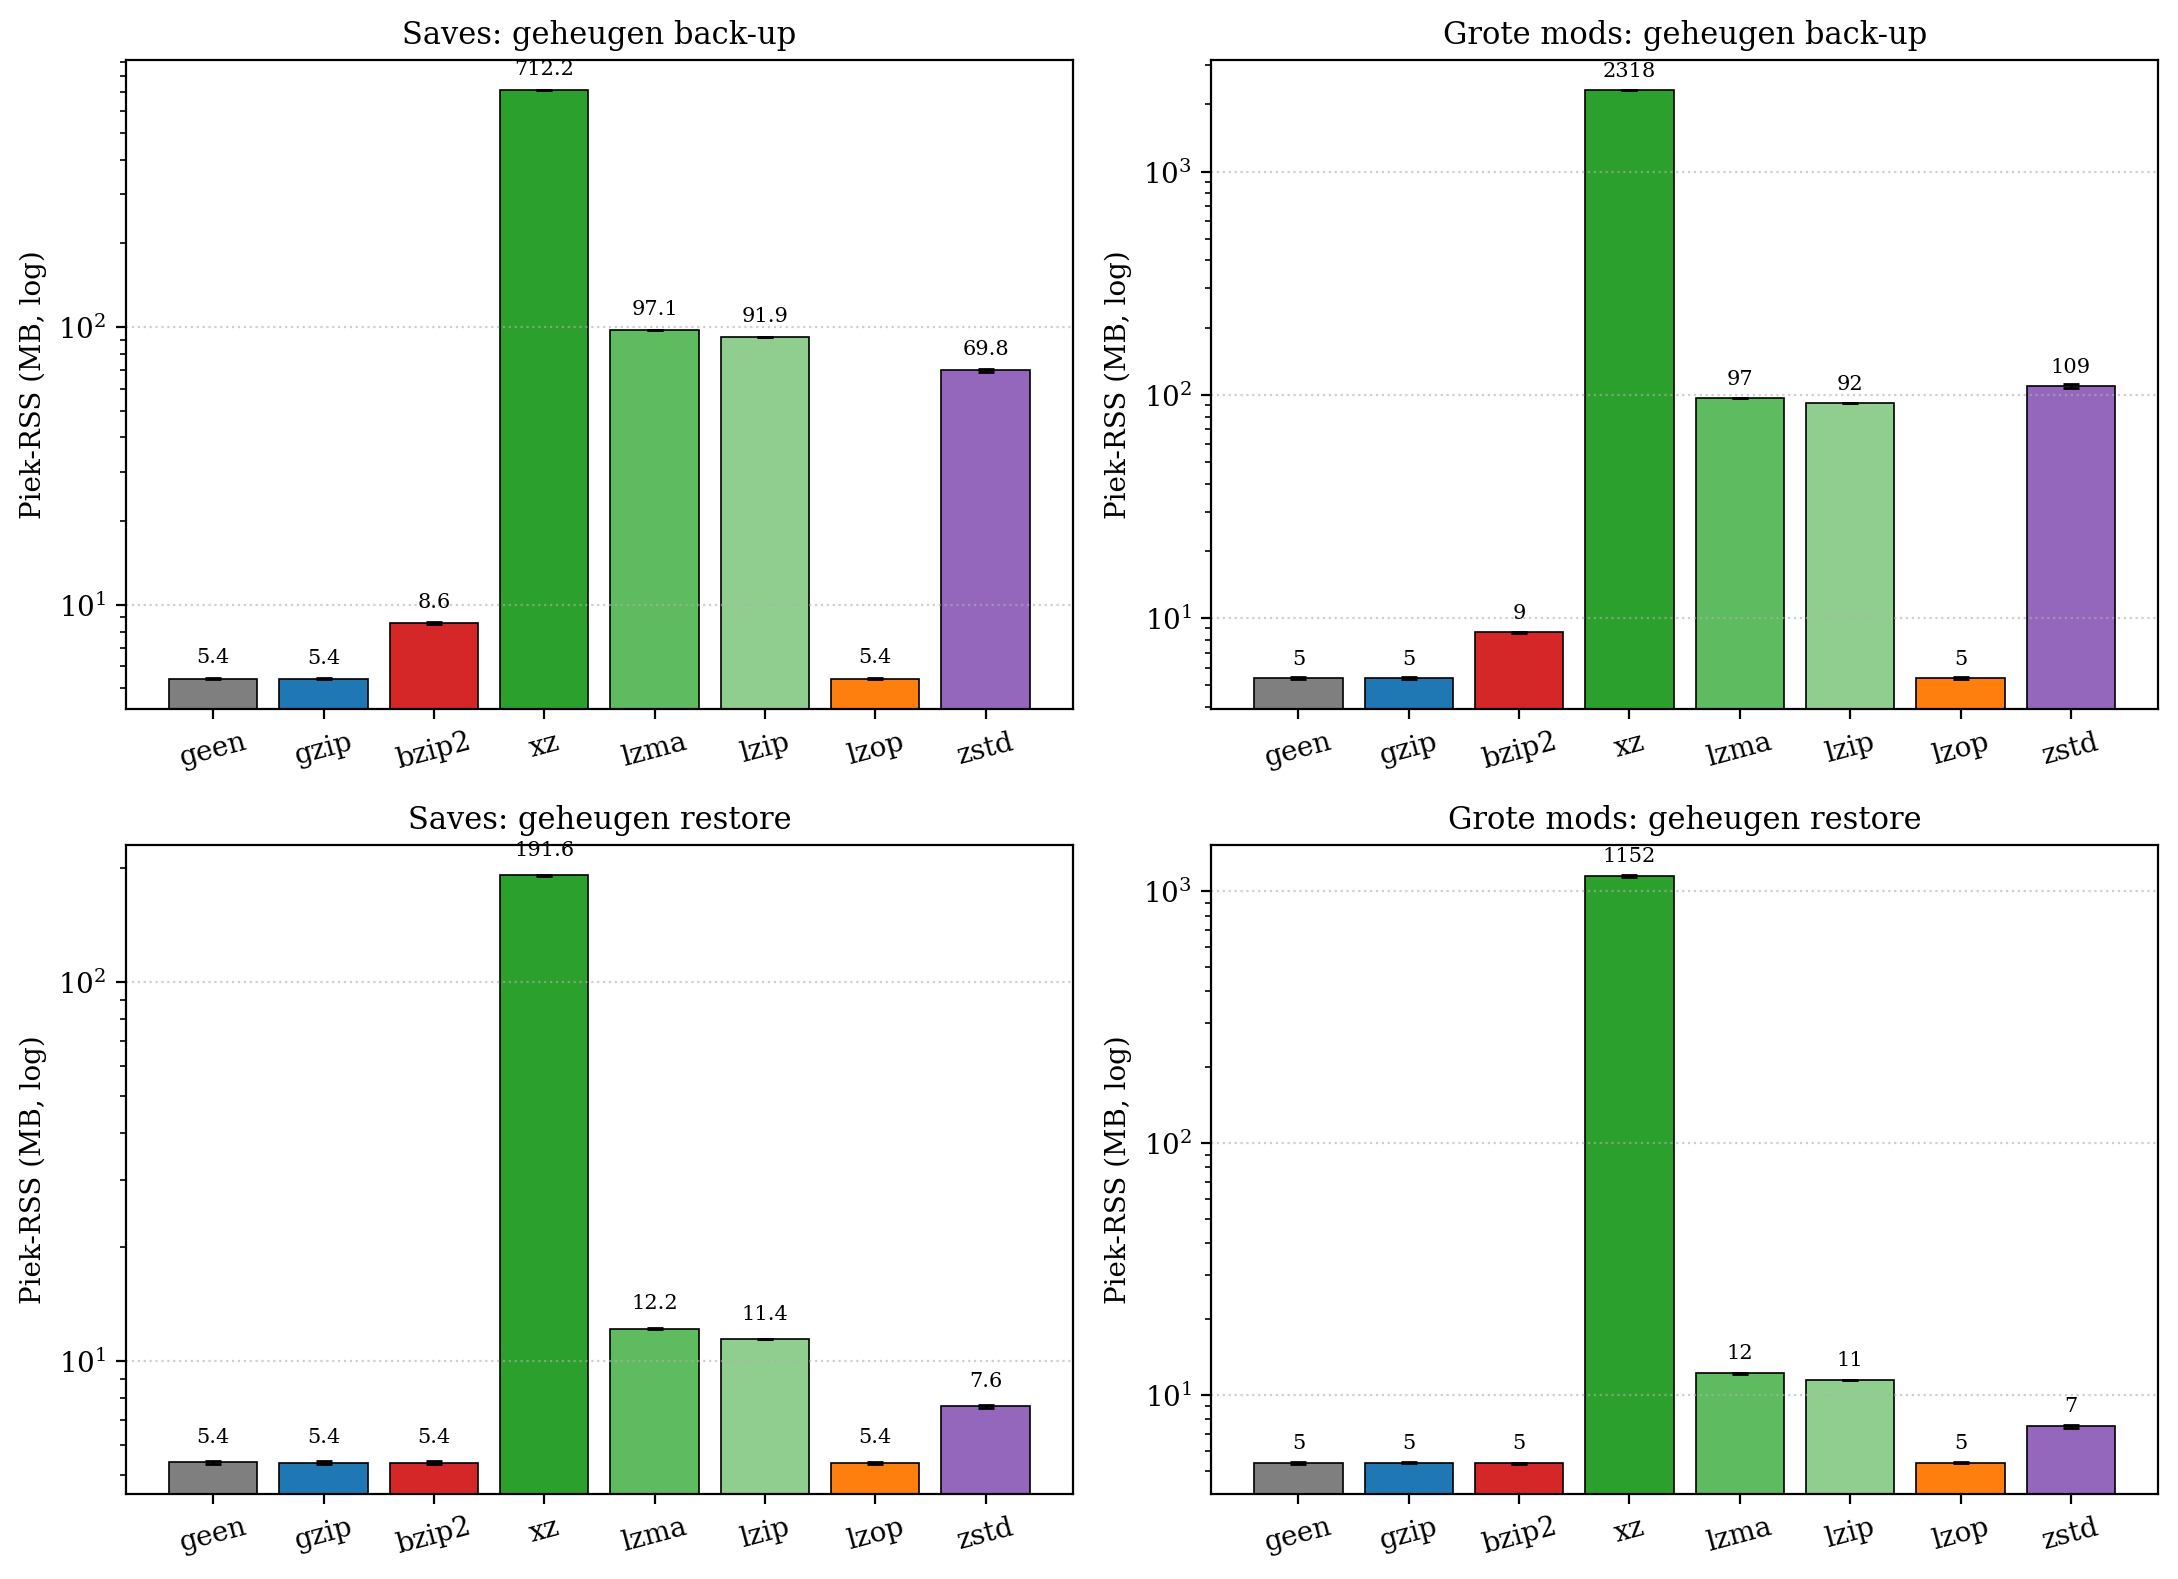
\includegraphics[width=\linewidth]{figures/fig_compression_mem.png}
    \caption{Piekgeheugengebruik per algoritme tijdens compressie (boven) en decompressie (onder). Y-as logaritmisch. De waarden zijn de hoogste piek over de hele dataset (alle saves of alle mods van één run).}
    \label{fig:compression-mem}
\end{figure}

\paragraph{Geheugen tijdens compressie.}
Het verschil tussen algoritmes is meer dan twee orden van grootte groot. \texttt{gzip} en \texttt{lzop} blijven beperkt tot $\sim$5~MB, identiek aan de ongecomprimeerde tar. \texttt{bzip2} gebruikt $\sim$9~MB, conform zijn vaste blokgrootte van 900~kB en zijn BWT-werkruimte. De LZMA-familie ligt rond $\sim$92 -- 97~MB (\texttt{lzma}, \texttt{lzip}) door het standaard woordenboek-formaat. \texttt{zstd} gebruikt $\sim$70 -- 110~MB. \texttt{xz} springt eruit met $\sim$712~MB op de saves en $\sim$2{,}3~GB op de mods. Dit enorm geheugengebruik is het gevolg van de combinatie van LZMA's groot woordenboek en de multithreading-strategie van \texttt{xz}, die per thread een eigen woordenboek bijhoudt.

\paragraph{Geheugen tijdens decompressie.}
Bij decompressie zakt het geheugengebruik aanzienlijk. Alle algoritmes behalve \texttt{xz} blijven onder 15~MB. \texttt{xz} gebruikt echter nog steeds $\sim$192~MB op saves en $\sim$1{,}15~GB op mods, omdat het voor parallelle decompressie eveneens meerdere woordenboeken in geheugen houdt. Single-threaded varianten \texttt{lzma} en \texttt{lzip} hebben slechts één woordenboek nodig en blijven daardoor onder de 13~MB. \texttt{bzip2} behoudt zijn kleine voetafdruk dankzij de blok-georiënteerde architectuur.

\subsection{Pareto-frontier: tijd versus archiefgrootte}
\label{subsec:pareto}

Een tweedimensionale afweging maakt de optimale keuzes veel gemakkelijker zichtbaar. Figuren~\ref{fig:pareto-backup} en~\ref{fig:pareto-restore} tonen elk algoritme als een punt in een ruimte met enerzijds tijd (logaritmisch) en anderzijds archiefgrootte. Algoritmes die op de Pareto-frontier liggen, zijn algoritmes waarvoor geen ander algoritme in deze test tegelijk sneller én kleiner is. Algoritmes die niet op de frontier liggen, zijn gedomineerd: er bestaat ten minste één alternatief dat in beide dimensies beter scoort.

\begin{figure}[h]
    \centering
    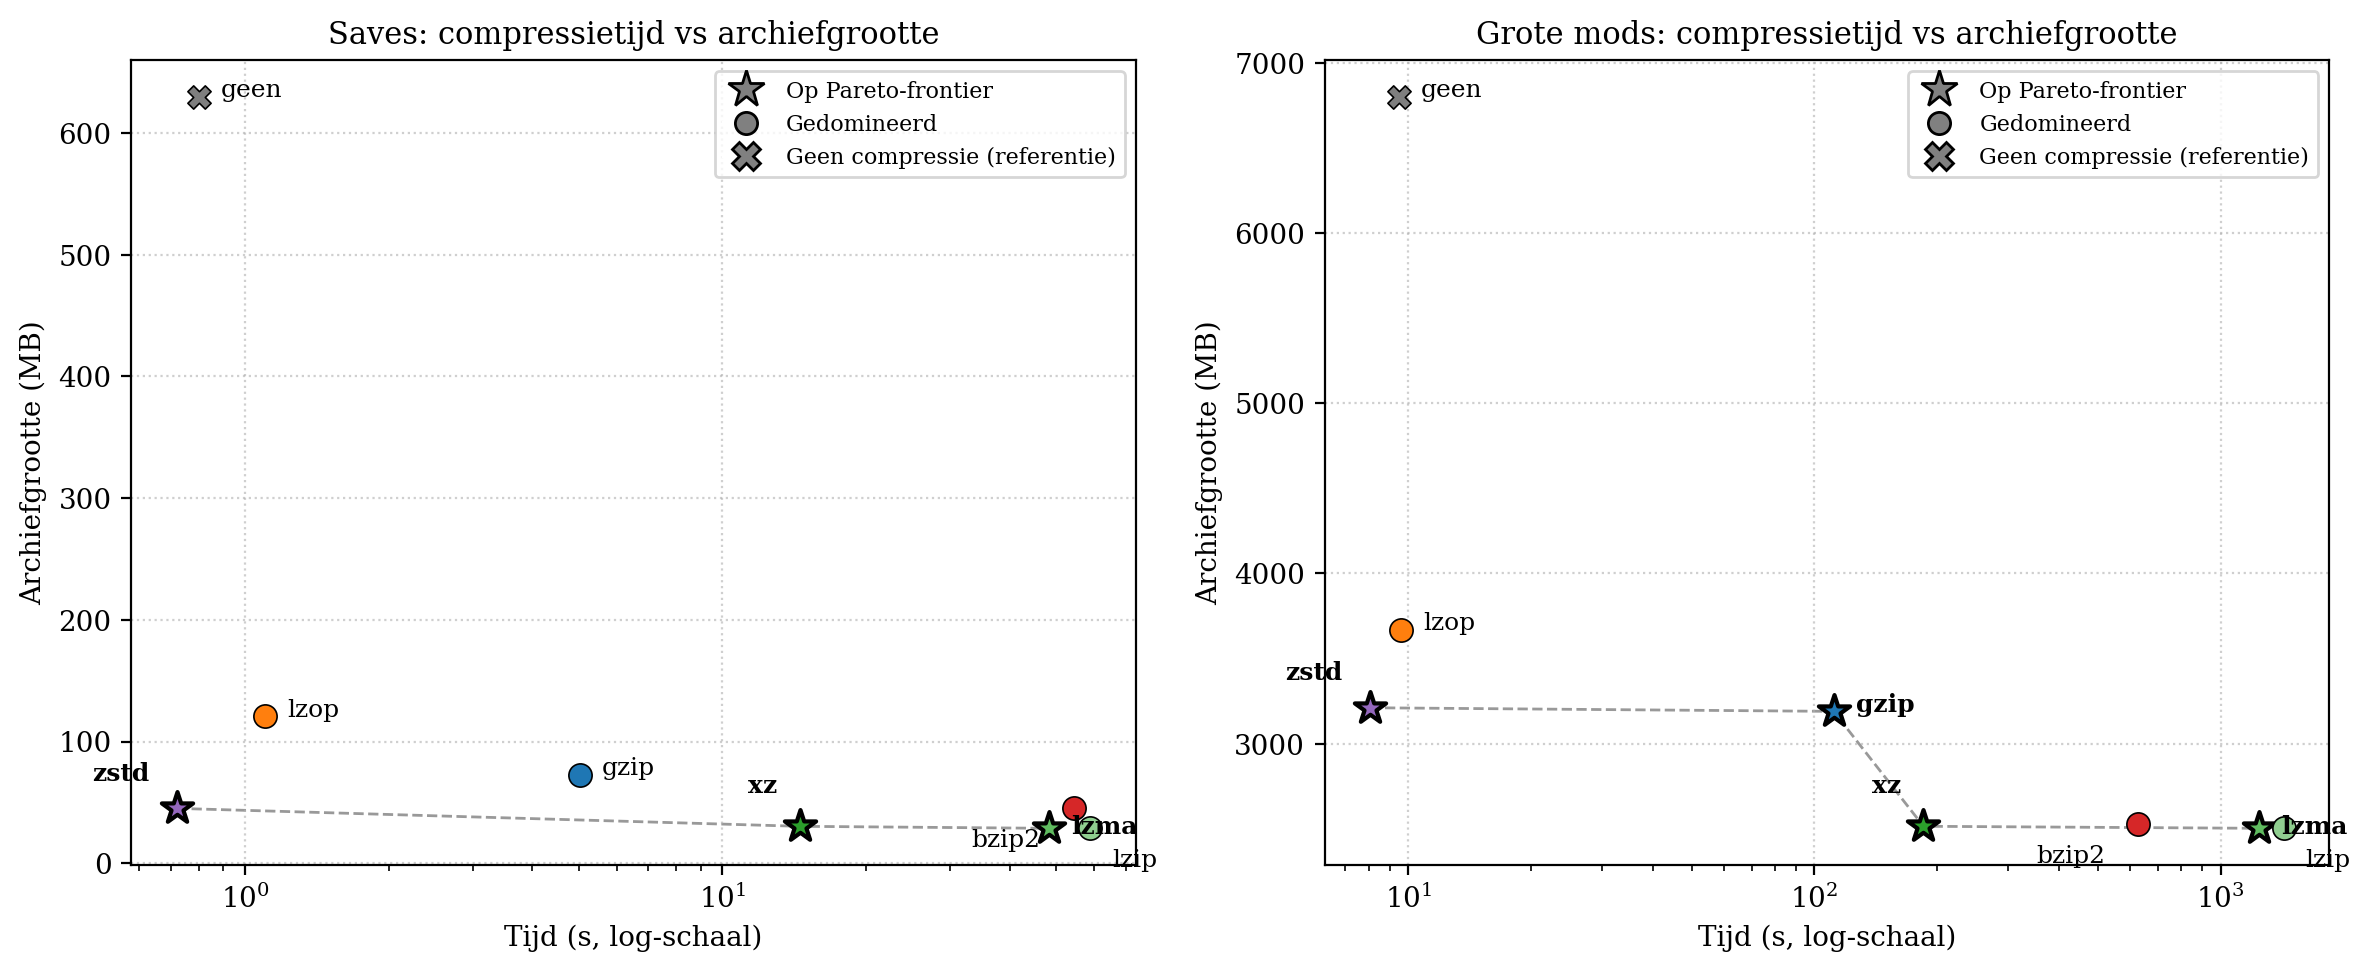
\includegraphics[width=\linewidth]{figures/fig_compression_pareto_backup.png}
    \caption{Pareto-frontier voor de back-upfase: compressietijd (x-as,
        log) tegenover archiefgrootte (y-as). Sterren markeren algoritmes op de Pareto-frontier; cirkels markeren gedomineerde algoritmes. Het kruis (geen compressie) wordt enkel getoond als referentie en werd uitgesloten uit de frontierberekening.}
    \label{fig:pareto-backup}
\end{figure}

\begin{figure}[h]
    \centering
    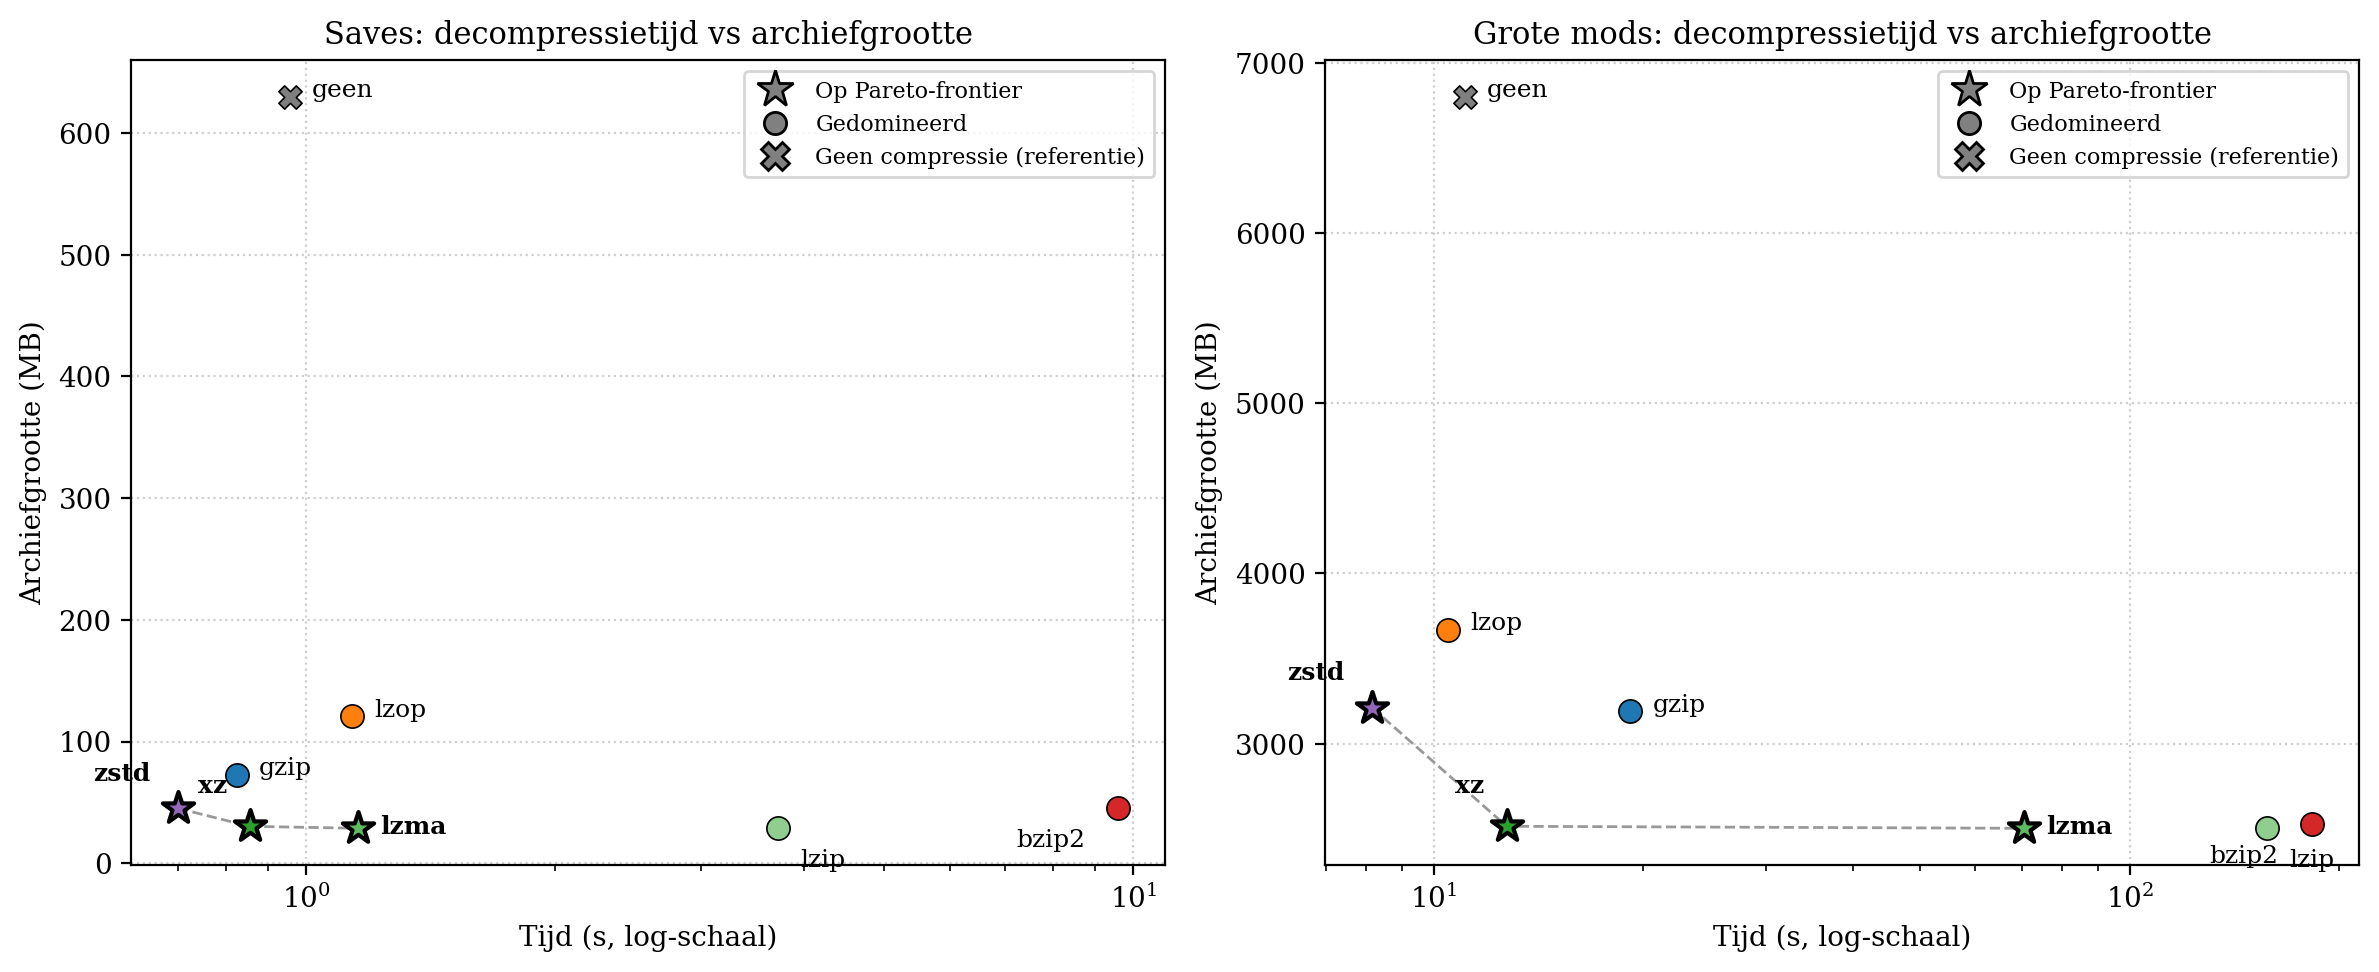
\includegraphics[width=\linewidth]{figures/fig_compression_pareto_restore.png}
    \caption{Pareto-frontier voor de restorefase: decompressietijd (x-as, log) tegenover archiefgrootte (y-as). Zelfde notatie als figuur~\ref{fig:pareto-backup}.}
    \label{fig:pareto-restore}
\end{figure}

\paragraph{Pareto-frontier voor de back-upfase.}
Bij beide datasets bestaat de back-upfrontier uit drie tot vier algoritmes. Voor de saves: \texttt{zstd} (snel, redelijke ratio), \texttt{xz} (middelmatige tijd, goede ratio), en \texttt{lzma}/\texttt{lzip} (traag, beste ratio). Voor de mods: \texttt{zstd}, \texttt{gzip}, \texttt{xz} en \texttt{lzma}. \texttt{lzop} en \texttt{bzip2} liggen onder de frontier en zijn dus gedomineerd: \texttt{lzop} wordt gedomineerd door \texttt{zstd} (zstd is sneller én kleiner), en \texttt{bzip2} wordt gedomineerd door \texttt{xz}.

\paragraph{Pareto-frontier voor de restorefase.}
De restoregrafieken geven een eenvoudiger beeld. Bij de saves: \texttt{zstd}, \texttt{xz} en \texttt{lzma} domineren alle overige algoritmes. \texttt{bzip2} en \texttt{lzip} vallen ver weg omdat hun decompressie traag is voor een ratio die geen voordeel oplevert ten opzichte van \texttt{xz}/\texttt{lzma}. Bij de mods is de frontier nog beknopter: \texttt{zstd}, \texttt{xz} en \texttt{lzma}, met \texttt{xz} duidelijk dominant boven \texttt{lzma} (kleinere ratio en snellere decompressie). \texttt{lzip} blijft op de frontier qua compressieratio bij sommige varianten, maar zijn $\sim$157~s decompressietijd op de mods plaatst hem ver buiten de praktische zone.

\subsection{Synthese en aanbeveling per dataset}
\label{subsec:compressie-conclusie}

Tabel~\ref{tab:compressie-summary} vat de belangrijkste meetwaarden
samen.

\begin{table}[h]
    \centering
    \caption{Compressie-algoritmes vergeleken op de volledige
        back-upmethode (totaal over de hele dataset). Tijden in seconden,
        grootte in MB, geheugen in MB.}
    \label{tab:compressie-summary}
    \small
    \begin{tabular}{lrrrrrrrr}
        \toprule
        & \multicolumn{4}{c}{\textbf{Saves ($\sim$629~MB origineel)}}
        & \multicolumn{4}{c}{\textbf{Mods ($\sim$6800~MB origineel)}} \\
        \cmidrule(lr){2-5}\cmidrule(lr){6-9}
        \textbf{Algoritme} & Comp. & Decomp. & Grootte & Mem
        & Comp. & Decomp. & Grootte & Mem \\
        \midrule
        geen           &   0{,}80  &   0{,}96  &   630 &     5
        &   9{,}48  &  12{,}58  &  6800 &     5 \\
        gzip           &   5{,}02  &   0{,}82  &    72 &     5
        & 111{,}51  &  19{,}14  &  3190 &     5 \\
        bzip2          &  54{,}42  &   9{,}59  &    45 &     9
        & 627{,}27  & 182{,}83  &  2530 &     9 \\
        xz             &  14{,}50  &   0{,}85  &    30 &   712
        & 185{,}59  &  12{,}73  &  2515 &  2318 \\
        lzma           &  48{,}23  &   1{,}16  &    29 &    97
        & 1245{,}18 &  70{,}43  &  2503 &    97 \\
        lzip           &  58{,}87  &   3{,}72  &    29 &    92
        & 1429{,}39 & 157{,}38  &  2505 &    92 \\
        lzop           &   1{,}10  &   1{,}14  &   121 &     5
        &   9{,}58  &  10{,}48  &  3670 &     5 \\
        zstd           &   0{,}72  &   0{,}70  &    45 &    70
        &   8{,}06  &   8{,}15  &  3211 &   109 \\
        \bottomrule
    \end{tabular}
\end{table}

\paragraph{Aanbeveling voor savegames.}
Bij de savegames komt \texttt{zstd} naar voren als de meest evenwichtige keuze: het comprimeert in $\sim$0{,}7~s tot $\sim$45~MB en decomprimeert in $\sim$0{,}7~s, met een geheugenvoetafdruk van $\sim$70~MB. Wie de allerkleinste archieven wil, kan kiezen voor \texttt{xz}, dat de archieven verder verkleint tot $\sim$30~MB met quasi-instantane decompressie ($\sim$0{,}85~s). De prijs is een back-uptijd die ongeveer 20 keer langer is en een geheugenpiek van $\sim$712~MB. Voor de typische gebruiker is dit een onnodig zwaar. \texttt{lzop} biedt geen meetbaar voordeel ten opzichte van \texttt{zstd} en wordt daarom afgeraden. \texttt{bzip2}, \texttt{lzma} en \texttt{lzip} verdedigen hun bestaansrecht hier niet: ze zijn allemaal aanzienlijk trager voor een zeer klein of onbestaand opslagvoordeel ten opzichte van \texttt{xz} of \texttt{zstd}.

\paragraph{Aanbeveling voor grote mods.}
Bij de mods wordt de keuze sterk beperkt door het feit dat de ratio's onderling weinig verschillen (een factor 1{,}5 tussen het beste en het slechtste algoritme), terwijl de tijden meer dan twee orden van grootte verschillen. \texttt{zstd} springt er hier sterk uit: het comprimeert sneller dan tar zonder compressie ($\sim$8~s tegenover $\sim$9{,}5~s), produceert een archief van $\sim$3{,}21~GB (een opslagbesparing van 53\%) en decomprimeert in slechts $\sim$8{,}2~s. De totale back-up + restore-cyclus duurt met \texttt{zstd} ongeveer 16 seconden, tegenover meer dan 26 minuten voor \texttt{lzip}. Het geheugengebruik blijft beperkt tot $\sim$109~MB, ruim binnen de mogelijkheden van een gemiddeld systeem.

De LZMA-varianten leveren bij de mods slechts $\sim$22\% kleinere archieven dan \texttt{zstd}, ten koste van een 23-keer langere back-uptijd (xz) tot zelfs een 177-keer langere back-uptijd (lzip). Voor de grote mods, waar ratios laag liggen door reeds gecomprimeerde assets, is deze niet acceptabel. \texttt{xz} blijft een goede keuze als de prioriteit op een zo klein mogelijke archiefgrootte ligt en het geheugengebruik van $\sim$2{,}3~GB geen probleem vormt, maar voor de typische thuisgebruiker is \texttt{zstd} duidelijk de optimale keuze.

\paragraph{Algemene observaties.}
Een aantal vaststellingen gelden voor beide datasets:

\begin{itemize}
    \item \textbf{\texttt{zstd} is in vrijwel alle dimensies de beste keuze.} Het haalt een goede compressieratio, comprimeert sneller dan ongecomprimeerde tar (door multithreading en verminderde I/O), decomprimeert minstens even snel, en blijft binnen aanvaardbare geheugengrenzen. Voor een back-upsysteem in een modlauncher is dit veruit het beste algoritme.
    \item \textbf{\texttt{lzop} wordt gedomineerd door \texttt{zstd}.} Vroeger was \texttt{lzop} de standaardkeuze voor maximale snelheid. \texttt{zstd} is op moderne hardware in vrijwel elke dimensie beter (sneller, kleinere archieven, vergelijkbaar geheugen).
    \item \textbf{\texttt{bzip2} en \texttt{lzip} zijn obsoleet voor deze werklast.} Hun trage decompressie (vooral voor \texttt{lzip}) maakt ze ongeschikt voor een rollbackscenario, terwijl ze geen compressievoordeel bieden ten opzichte van \texttt{xz} of \texttt{lzma}.
    \item \textbf{\texttt{xz} is een verdedigbare keuze voor maximaal kleine archieven}, mits het geheugengebruik geen probleem vormt. Voor mods is dit een aandachtspunt: een piek van $\sim$2{,}3~GB tijdens een back-up kan op een gamingsysteem merkbare impact hebben.
    \item \textbf{Grote mods comprimeren slecht door reeds gecomprimeerde assets.} De keuze van een agressief algoritme levert hier niet de winst op die ze bij saves geeft. Het is dus geen slecht idee om per datatype te differentiëren: voor saves kan een agressiever algoritme zinvol zijn, voor mods is een snel algoritme zoals \texttt{zstd} duidelijk de beste optie.
\end{itemize}


\section{Algemene ontwerprichtlijnen}
\label{sec:ontwerprichtlijnen}

In deze afsluitende sectie worden de bevindingen uit de analyse van de back-upmethodes (sectie~\ref{sec:synthese}) en de analyse van de compressie-algoritmes (sectie~\ref{subsec:compressie-conclusie}) samengebracht tot één set van ontwerprichtlijnen voor een back-up\-systeem in een modlauncher. De richtlijnen worden gegroepeerd rond drie thema's: de keuze van de back-upmethode, de keuze van het compressie-algoritme, en algemene architecturele principes.

\subsection{Richtlijnen voor de keuze van back-upmethode}

\begin{enumerate}
    \item \textbf{Snapshotting heeft de voorkeur wanneer het bestandssysteem dit toelaat.} Een copy-on-write snapshot-mechanisme (zoals btrfs of zfs) levert in alle geteste dimensies de beste resultaten: voorspelbare en lage back-up\-kost per back-uppunt, quasi-instantane rollbacks (in de orde van tientallen milliseconden), lage fysieke opslagvoetafdruk dankzij blok\-niveau-deduplicatie, en minimaal CPU- en geheugengebruik. Geen enkele andere geteste methode kan deze combinatie evenaren.
    \item \textbf{Wanneer snapshots niet beschikbaar zijn, is een incrementele methode het beste compromis.} De back-uptijd per punt is laag en het opslaggebruik is zuiniger dan dat van een volledige of differentiële strategie. De per-back-uppuntanalyse heeft echter aangetoond dat de cumulatieve restoretijd merkbaar oploopt naarmate er meer incrementen zijn. Een periodieke nieuwe basis-back-up is daarom wenselijk om de restoretijd binnen bruikbare grenzen te houden.
    \item \textbf{Een differentiële strategie wordt afgeraden.} De analyse heeft aangetoond dat differentieel geen meetbaar voordeel oplevert ten opzichte van incrementeel: de archieven groeien cumulatief met elke nieuwe back-up, het opslaggebruik ligt hoger, de back-uptijd is langer, en de restoretijd is nauwelijks beter dan bij incrementeel.
    \item \textbf{Een volledige back-up zonder bijkomende logica is zelden zinvol.} Voor de werklast van een modlauncher levert deze methode geen voordeel op. De methode is enkel verdedigbaar voor scenario's waar de dataset uitzonderlijk klein en eenmalig is.
\end{enumerate}

\subsection{Richtlijnen voor de keuze van compressie-algoritme}

\begin{enumerate}\setcounter{enumi}{4}
    \item \textbf{\texttt{zstd} is de standaardkeuze voor compressie.} Het algoritme laat op vrijwel geen enkele dimensie een steek vallen. Op de moddataset comprimeert het zelfs sneller dan een ongecomprimeerde tar-back-up, dankzij de combinatie van multithreading en de kleinere I/O-belasting van een gecomprimeerd archief. De compressieratio ligt voor saves bij $\sim$0{,}07 en voor mods bij $\sim$0{,}47, met een decompressietijd die in beide gevallen de snelste is van alle geteste algoritmes en een geheugengebruik die ruim binnen de mogelijkheden van een gamingsysteem blijft.
    \item \textbf{\texttt{xz} is de optionele keuze voor maximale opslagbesparing.} Voor gebruikers waarvoor archiefgrootte primair is en geheugengebruik geen probleem is, levert \texttt{xz} archieven op die nog $\sim$22\% kleiner zijn dan die van \texttt{zstd}.
    \item \textbf{De overige algoritmes worden afgeraden.} \texttt{lzop} wordt in alle dimensies gedomineerd door \texttt{zstd}. \texttt{gzip} levert geen voordeel ten opzichte van \texttt{zstd} en is bovendien single-threaded. \texttt{bzip2} en \texttt{lzip} hebben een trage decompressie die ze ongeschikt maakt voor een rollback- scenario. \texttt{lzma} is in essentie hetzelfde algoritme als \texttt{xz} maar zonder multithreading en is daardoor altijd trager.
    \item \textbf{Differentieer per datatype.} Saves comprimeren uitstekend (ratio $\sim$0{,}07 met \texttt{zstd}); mods bevatten reeds gecomprimeerde assets en leveren bij geen enkel algoritme een ratio onder $\sim$0{,}37 op. Een agressiever algoritme inzetten voor de mods levert dus weinig extra winst op, terwijl de tijdkost dramatisch toeneemt. Een back-upsysteem kan eventueel een ander algoritme inzetten naargelang het type data, maar in de praktijk is \texttt{zstd} voor beide gevallen een zeer goede optie.
\end{enumerate}

\subsection{Algemene architecturele principes}

\begin{enumerate}\setcounter{enumi}{8}
    \item \textbf{Het back-upsysteem moet lokaal functioneren.} Zoals besproken in sectie~\ref{subsec:geen-cloud} is een cloud-gebaseerde back-up niet geschikt voor de context van een modlauncher: het spel kan offline gespeeld worden en mods kunnen meerdere gigabytes groot zijn. De back-up moet dus kunnen plaatsvinden zonder afhankelijk te zijn van een netwerkverbinding. Een optionele synchronisatie naar een externe locatie kan worden toegevoegd, maar mag geen vereiste zijn voor de basisfunctionaliteit.
    \item \textbf{De combinatie van methode en compressie is grotendeels orthogonaal.} Voor opstellingen met btrfs blijft de snapshotmethode primair en is compressie niet van toepassing (btrfs ondersteunt zelf transparante compressie, wat een afzonderlijke optimalisatie is buiten het bereik van dit onderzoek). Voor opstellingen waarin tar wordt gebruikt, levert de combinatie \texttt{tar + zstd} (incrementeel) de beste algemene afweging op: \texttt{zstd} voegt zo weinig extra rekentijd toe dat de gunstige eigenschappen van de incrementele methode behouden blijven, terwijl de archiefgrootte significant afneemt.
    \item \textbf{Voorspelbaarheid is een ontwerp\-eigenschap.} De analyses tonen aan dat snapshot-back-ups quasi-constante kosten hebben per back-up, terwijl tar-gebaseerde methodes meer variabiliteit vertonen, vooral de volledige restore op grote archieven. Voor een back-upsysteem dat geautomatiseerd wordt (bijvoorbeeld bij elke mod-update), is voorspelbaarheid een belangrijke kwaliteit: de gebruiker mag niet geconfronteerd worden met onverwachte wachttijden die de spelervaring verstoort.
\end{enumerate}

\subsection{Samenvatting van de aanbevolen configuratie}

Op basis van het bovenstaande wordt de volgende standaardconfiguratie voor een modlauncher\-back\-up\-systeem aanbevolen:

\begin{itemize}
    \item \textbf{Primaire methode:} btrfs-snapshots, indien het bestandssysteem dit ondersteunt. Snapshots bij elke savegame en bij elke mod-installatie of -update.
    \item \textbf{Secundaire methode:} incrementele \texttt{tar}- back-ups gecomprimeerd met \texttt{zstd}, met periodiek een nieuwe basis-back-up om de restoretijd onder controle te houden.
    \item \textbf{Locatie:} lokaal, met een optionele synchronisatiemodule naar externe opslag voor wie dat wenst.
\end{itemize}

\chapter{\IfLanguageName{dutch}{Evaluatie en validatie van het prototype}{Evaluation and validation of the prototype}}%
\label{ch:evaluatie-prototype}

\section{Inleiding}
\label{sec:eval-inleiding}

Dit hoofdstuk evalueert het prototype dat is ontwikkeld op basis van de ontwerprichtlijnen uit het vorige hoofdstuk. De evaluatie focust op drie dimensies: functionele correctheid, conformiteit met de geformuleerde ontwerprichtlijnen, en bruikbaarheid van de gebruikersinterface.

\subsection{Afbakening en motivering van de scope}

De tool die in dit hoofdstuk wordt geëvalueerd, ondersteunt op dit moment één back-up-methode: incrementele tar+zstd. Btrfs-snapshotting werd in het finale prototype weggelaten. De doorslaggevende reden is: het aandeel computergebruikers dat een btrfs-bestandssysteem gebruikt is bijzonder laag, waardoor de relevantie van deze methode voor de doelgroep (KSP-spelers in het algemeen) beperkt blijft. Btrfs-ondersteuning wordt om die reden beschouwd als een uitbreiding voor toekomstig werk, detectie voor het type bestandssysteem is wel al geïmplementeerd. Sectie~\ref{sec:eval-conformiteit} gaat hier dieper op in bij de bespreking van de eerste ontwerprichtlijn.

Een tweede afbakening betreft de evaluatiemethodologie. De UX-evaluatie in sectie~\ref{sec:eval-heuristiek} steunt op een heuristische analyse volgens de tien usability-principes van Nielsen, uitgevoerd door de ontwikkelaar zelf op basis van praktisch gebruik van het prototype op een werkelijke KSP-installatie met meer dan 100 mods en verschillende savegames.

\subsection{Keuze van de programmeertaal}
\label{subsec:eval-taal}

Voor de implementatie van het prototype werd Python gekozen. Deze keuze verdient toelichting, omdat CKAN (de bestaande modlauncher voor KSP) in C\# is geschreven. Vier overwegingen lagen aan de basis van de keuze voor Python in deze fase:

\begin{itemize}
    \item \textbf{Aard van de werklast.} De kernoperaties van de tool (\texttt{btrfs subvolume snapshot}, \texttt{tar}, \texttt{zstd}, \texttt{rsync}, \texttt{findmnt}) zijn allemaal externe binaries die via shell-commando's worden aangeroepen. De programmeertaal speelt hier geen rol in de prestaties, alle rekenintensieve werk gebeurt in de aangeroepen tools. Pythons \texttt{subprocess}-module biedt de meest directe en leesbare integratie voor dit soort patronen op Linux.
    \item \textbf{Snelheid van ontwikkeling.} Voor een proof of concept weegt ontwikkelsnelheid zwaarder dan distributiegemak. Pythons rijke standaardbibliotheek (\texttt{json}, \texttt{pathlib}, \texttt{dataclasses}, \texttt{subprocess}) en PySide6 voor Qt laten toe om in een beperkte tijd tot een werkende GUI te komen.
    \item \textbf{Distributievereisten zijn beperkt voor een PoC.} Het belangrijkste voordeel dat C\# zou bieden, een single- binary distributie via .NET, is voor een prototype dat op één testsysteem moet draaien geen doorslaggevend criterium.
    \item \textbf{CKAN-integratie als toekomstig werk.} Een rechtstreekse integratie van het back-upsysteem in CKAN is het ultieme einddoel van dit type tool, maar valt buiten de scope van dit prototype. Wanneer die integratie in de toekomst wordt ondernomen, is een C\#-implementatie de natuurlijke keuze. Voor de huidige fase, waarin de focus ligt op het valideren van de ontwerprichtlijnen via een werkende standalone tool, biedt Python de beste route.
\end{itemize}

De combinatie van Python met PySide6 (Qt for Python) levert een moderne dark-themed GUI op die past bij hedendaagse desktops. Figuur~\ref{fig:eval-home} toont het hoofdscherm van het prototype waarin een KSP-installatie met 113 mods is geconfigureerd.

\begin{figure}[h]
    \centering
    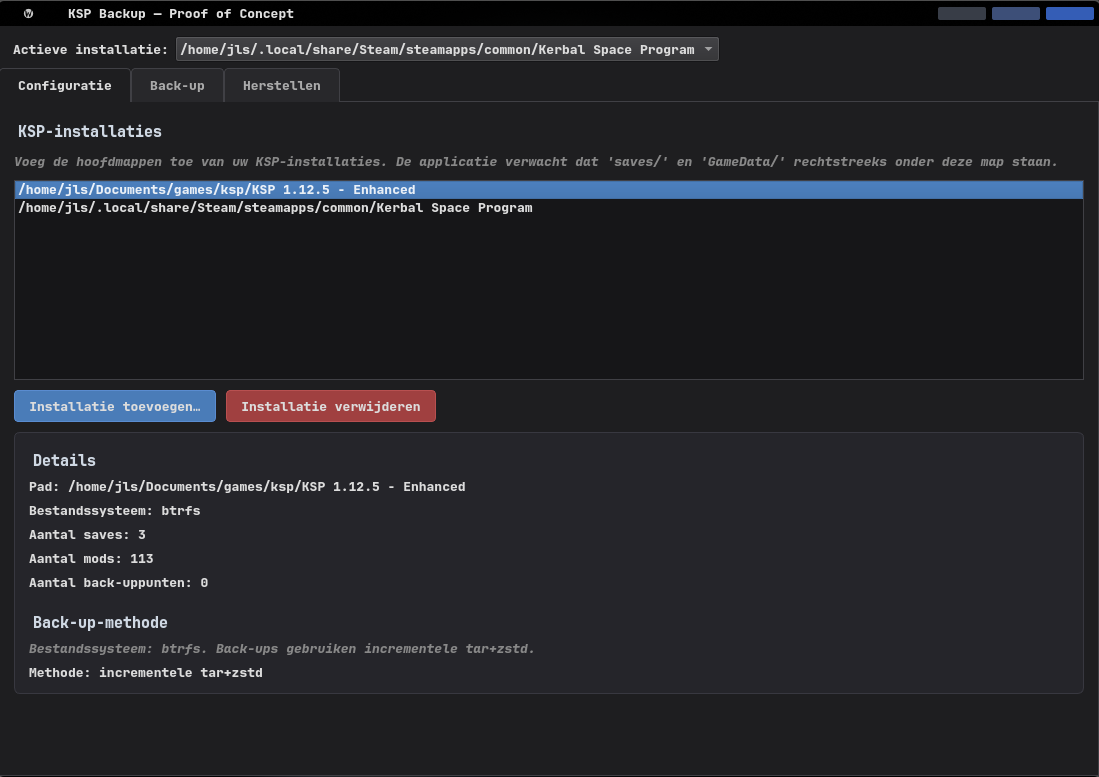
\includegraphics[width=0.95\linewidth]{home_screen.png}
    \caption{Configuratie-scherm van het prototype, met een werkelijke KSP mod-installatie van 20{,}5~GB en 113 mods.}
    \label{fig:eval-home}
\end{figure}


\section{Functionele evaluatie via testmatrix}
\label{sec:eval-functioneel}

Om de functionele correctheid van het prototype systematisch te beoordelen, werd een testmatrix opgesteld die elk afzonderlijk aspect van de tool valideert. De testen zijn gegroepeerd in vier clusters: basis back-up en restore, selectie en interface, configuratie en metadata, en edge cases met foutafhandeling. Elk testgeval beschrijft een doel, een uitgevoerde stap en een verwacht resultaat, waarna het werkelijke gedrag wordt gerapporteerd.

\subsection{Cluster 1: Basis back-up en restore}

Tabel~\ref{tab:eval-cluster1} toont de testen van de kernfunctionaliteiten. Deze testen werden uitgevoerd op een werkelijke KSP-installatie met 113 mods die 20{,}5~GB omvatten. Eén van de testen (volledige back-up van de mod-set) leverde meteen ook een nuttige indicatieve meting op: de back-up van alle 113 mods (level~0) duurde ongeveer 37{,}5~seconden en resulteerde in een gecomprimeerd archief van 10{,}3~GB. Een volledige restore van die set duurde ongeveer 25~ seconden. Deze cijfers fungeren in dit hoofdstuk niet als benchmark, maar als bewijs dat het prototype daadwerkelijk werkt op realistische werklasten zonder de UI te bevriezen.

\begin{table}[h]
    \centering
    \caption{Cluster 1: basis back-up en restore.}
    \label{tab:eval-cluster1}
    \small
    \begin{tabular}{p{0.32\linewidth}p{0.42\linewidth}p{0.16\linewidth}}
        \toprule
        \textbf{Testgeval} & \textbf{Verwacht resultaat} & \textbf{Status} \\
        \midrule
        Eerste back-up van een save als level 0 & Volledig basisarchief wordt aangemaakt en metadata-entry met \texttt{increment\_level=0}. & Geslaagd \\
        Eerste back-up van een mod als level 0 & Identiek aan vorige test, maar voor een mod-map onder \texttt{GameData/}. & Geslaagd \\
        Tweede back-up van hetzelfde item creëert level 1 & Tar gebruikt het bestaande snar-bestand en produceert enkel de wijzigingen sinds de vorige back-up. & Geslaagd \\
        Restore van een level-0-punt & Werkmap wordt teruggebracht naar de toestand van het basisarchief. & Geslaagd \\
        Restore van een level-2-punt & Drie archieven (level 0, 1 en 2) worden sequentieel uitgepakt; de werkmap reflecteert de cumulatieve toestand. & Geslaagd \\
        Multi-item back-up (saves en mods) in één actie & Alle geselecteerde items krijgen dezelfde \texttt{set\_id} en worden gegroepeerd weergegeven in de restore-lijst. & Geslaagd \\
        Back-up en restore van een grote werklast (20{,}5~GB, 113 mods) & Operatie voltooit zonder UI-bevriezing; gemeten $\sim$37{,}5~s back-up, $\sim$25~s restore. & Geslaagd \\
        \bottomrule
    \end{tabular}
\end{table}

Figuur~\ref{fig:eval-backup-progress} toont het back-up-scherm tijdens een volledige back-up van de 113 mods. De vooruitgangsbalk en de live log onderaan houden de gebruiker geïnformeerd zonder dat de UI bevriest. De aangeroepen \texttt{tar}-processen draaien op een achtergrondthread via Qt's \texttt{QThread}-mechanisme.

\begin{figure}[h]
    \centering
    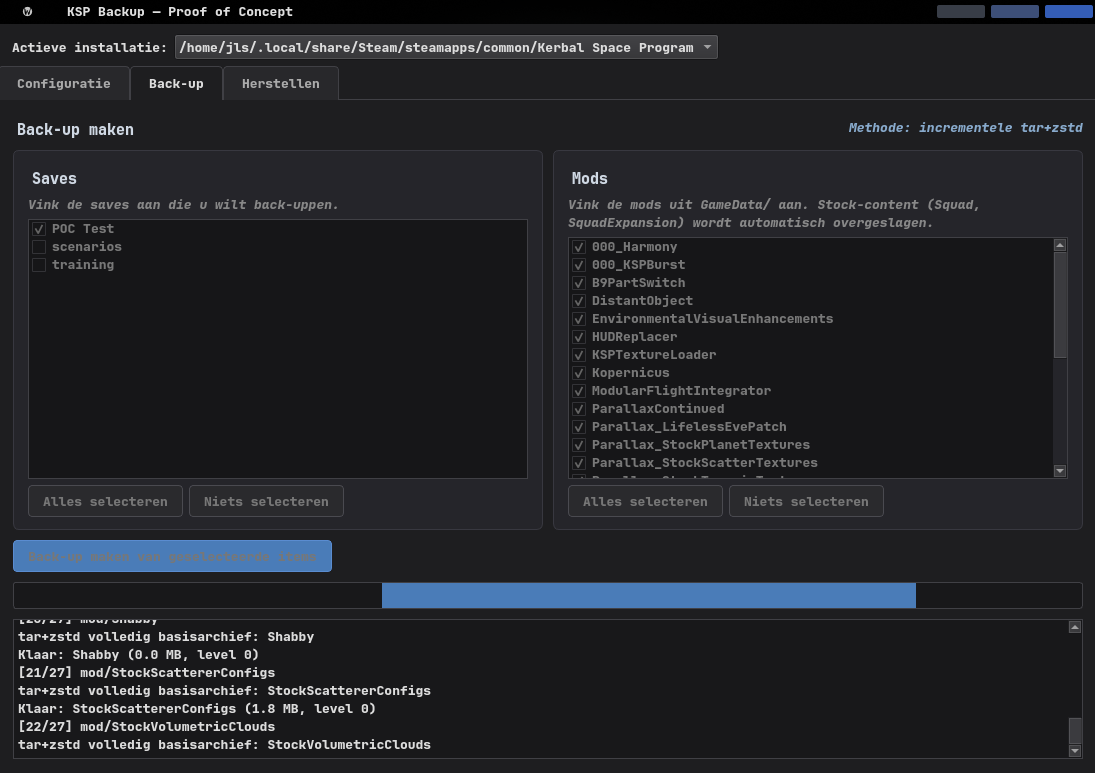
\includegraphics[width=0.95\linewidth]{backup_scherm_tijdens_backup.png}
    \caption{Back-up-scherm tijdens uitvoering. De progressbar toont dat de operaties nog bezig zijn en de log onderaan rapporteert per item de status en grootte. De gebruikersinterface blijft responsief tijdens de hele operatie.}
    \label{fig:eval-backup-progress}
\end{figure}

\subsection{Cluster 2: Selectie en interface}

Tabel~\ref{tab:eval-cluster2} verzamelt de testen rond gebruikersinteractie en visuele weergave.

\begin{table}[h]
    \centering
    \caption{Cluster 2: selectie en interface.}
    \label{tab:eval-cluster2}
    \small
    \begin{tabular}{p{0.32\linewidth}p{0.42\linewidth}p{0.16\linewidth}}
        \toprule
        \textbf{Testgeval} & \textbf{Verwacht resultaat} & \textbf{Status} \\
        \midrule
        Selectie van meerdere saves uit een lijst & Enkel de aangevinkte saves worden in de back-up opgenomen. & Geslaagd \\
        Stock-content (\texttt{Squad}, \texttt{SquadExpansion}) wordt overgeslagen & Deze mappen verschijnen niet in de mod-lijst. & Geslaagd \\
        Multi-select restore over verschillende back-up-sets & Items uit verschillende sets kunnen tegelijk geselecteerd en in één actie hersteld worden. & Geslaagd \\
        Boomstructuur groepeert per back-up-actie en daarbinnen per type & Restore-tab toont sets met daaronder ``Saves''- en ``Mods''-groepen. & Geslaagd \\
        Groene cirkel toont het huidige back-uppunt & Na een back-up of restore krijgt het corresponderende back-uppunt een groene markering; oudere punten van hetzelfde item verliezen die markering. & Geslaagd \\
        \bottomrule
    \end{tabular}
\end{table}

Figuur~\ref{fig:eval-backup-screen} illustreert het selectiescherm na voltooiing van een back-up van alle 113 mods. De saves- en mods-kolommen tonen aanvinkbare lijsten, stock-mappen zoals \texttt{Squad} ontbreken. Figuur~\ref{fig:eval-restore-after} toont de restore-tab na een herstel van een save naar level 2: de groene cirkel naast het zonet herstelde punt geeft duidelijk aan welk punt op dit moment actief is in de werkmap.

\begin{figure}[h]
    \centering
    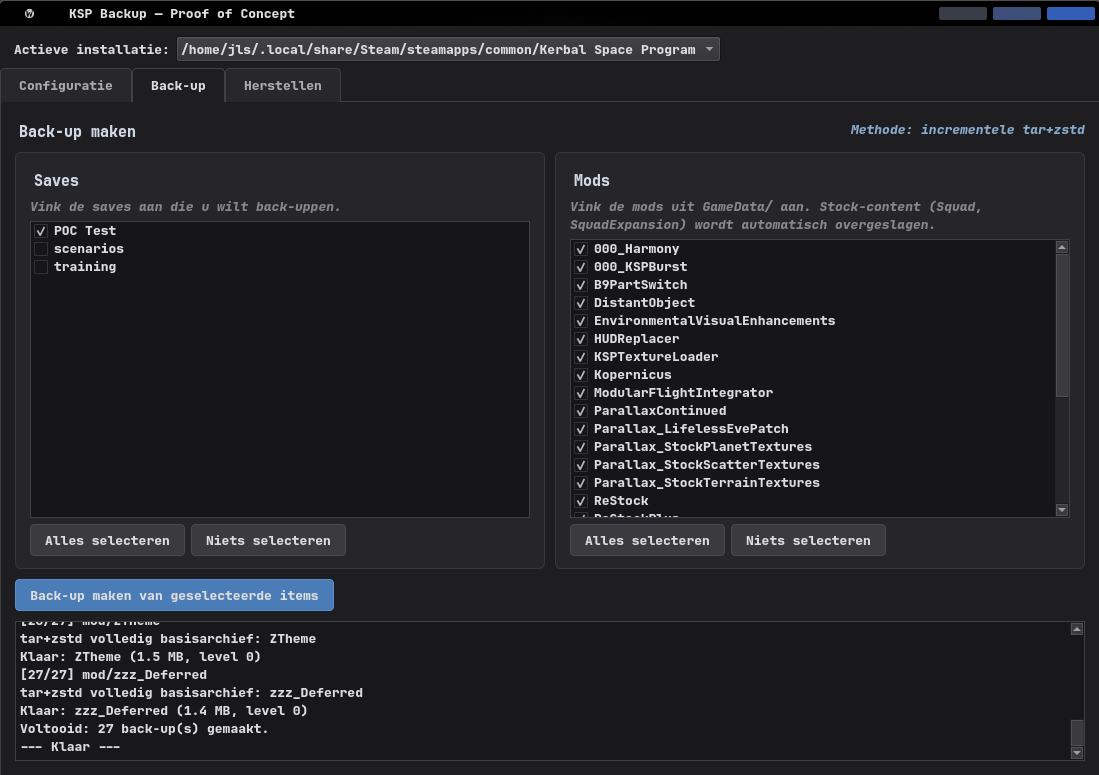
\includegraphics[width=0.95\linewidth]{backup_screen.png}
    \caption{Back-up-scherm met selectie-interface. Saves en mods staan in afzonderlijke kolommen. De methode (incrementele tar+zstd) wordt rechtsbovenin altijd getoond.}
    \label{fig:eval-backup-screen}
\end{figure}

\begin{figure}[h]
    \centering
    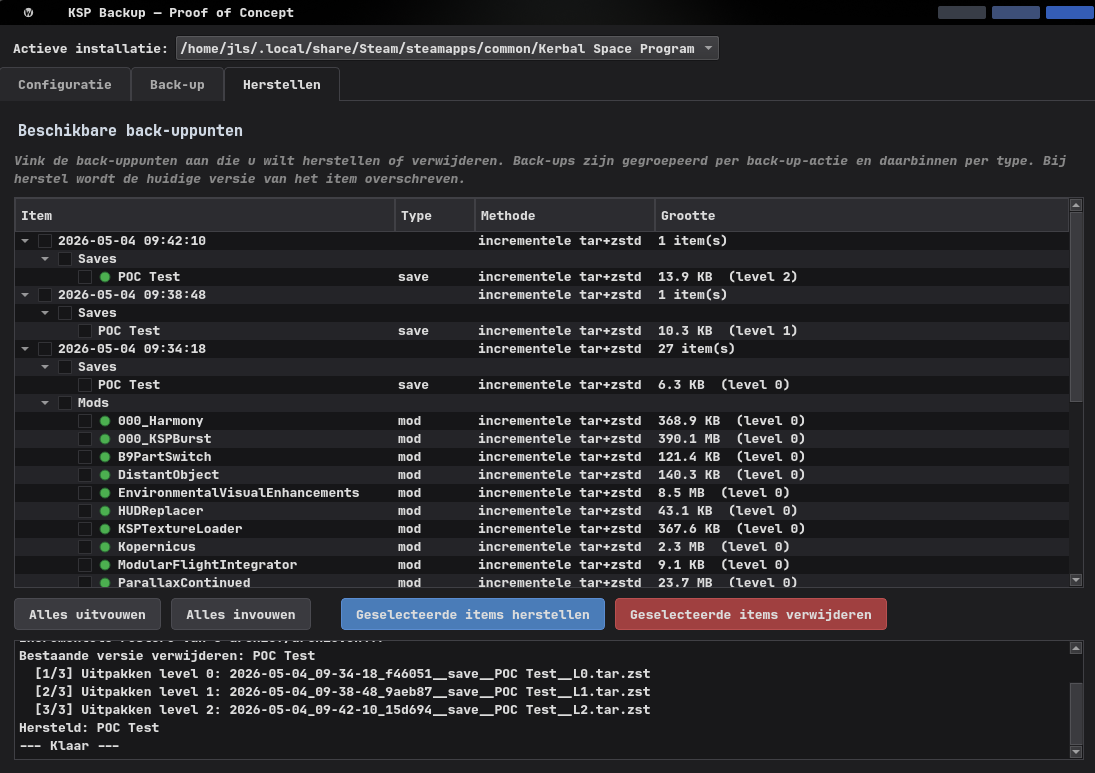
\includegraphics[width=0.95\linewidth]{restore_screen_na_restore_van_level_3.png}
    \caption{Restore-tab na een herstel naar een level-2-punt. De log onderaan toont dat drie archieven sequentieel werden uitgepakt. De groene cirkel naast het herstelde punt (level 2) markeert het als de huidige toestand; de oudere punten van datzelfde item zijn niet meer gemarkeerd.}
    \label{fig:eval-restore-after}
\end{figure}

\subsection{Cluster 3: Configuratie en metadata}

Tabel~\ref{tab:eval-cluster3} verzamelt de testen rond configuratie en metadata. De testen in dit cluster tonen aan dat de scheiding tussen globale en per-installatie state correct werkt. De globale configuratie in \texttt{\textasciitilde/.config/ksp-backup/installations.json} beperkt zich bewust tot een lijst van paden naar bekende installaties. Alle eigenlijke back-upmetadata staat in de \texttt{metadata.json} binnen elke KSP-installatie zelf.


\begin{table}[h]
    \centering
    \caption{Cluster 3: configuratie en metadata.}
    \label{tab:eval-cluster3}
    \small
    \begin{tabular}{p{0.32\linewidth}p{0.42\linewidth}p{0.16\linewidth}}
        \toprule
        \textbf{Testgeval} & \textbf{Verwacht resultaat} & \textbf{Status} \\
        \midrule
        Toevoegen van een KSP-installatie persisteert na herstart & De installatie verschijnt opnieuw in de lijst na het sluiten en opnieuw openen van de applicatie. & Geslaagd \\
        Verwijderen van een installatie raakt de bestanden niet aan & De installatie wordt enkel uit de globale lijst gehaald; de KSP-folder en \texttt{Backups/}-submap blijven intact. & Geslaagd \\
        Beheren van meerdere installaties tegelijk & Verschillende KSP-installaties kunnen onafhankelijk worden geconfigureerd; elke installatie heeft zijn eigen \texttt{metadata.json}. & Geslaagd \\
        Detectie van het bestandssysteem & \texttt{findmnt} geeft \texttt{btrfs} terug voor de getoonde installatie; de configuratie-tab rapporteert dit correct (zie figuur~\ref{fig:eval-home}). & Geslaagd \\
        \bottomrule
    \end{tabular}
\end{table}

\subsection{Cluster 4: Edge cases en foutafhandeling}

\begin{table}[h]
    \centering
    \caption{Cluster 4: edge cases en foutafhandeling.}
    \label{tab:eval-cluster4}
    \small
    \begin{tabular}{p{0.32\linewidth}p{0.42\linewidth}p{0.16\linewidth}}
        \toprule
        \textbf{Testgeval} & \textbf{Verwacht resultaat} & \textbf{Status} \\
        \midrule
        Verwijderen van een level 0 leidt tot cascade-cleanup & Het basisarchief, alle latere incrementen van datzelfde item én het snar-bestand worden samen verwijderd. & Geslaagd \\
        Verwijderen van enkel een tussenliggende increment behoudt de chain & Het basisarchief en eventueel andere incrementen blijven bruikbaar; het snar-bestand blijft eveneens behouden. & Geslaagd \\
        Bevestigingsdialoog vóór restore en delete & Een dialoog toont alle te overschrijven of te verwijderen items vóór de uitvoering en vraagt expliciet om bevestiging. & Geslaagd \\
        Cascade-waarschuwing bij verwijderen van een level 0 & De delete-dialoog vermeldt expliciet welke afhankelijke incrementen mee zullen worden verwijderd. & Geslaagd \\
        \bottomrule
    \end{tabular}
\end{table}

Tabel~\ref{tab:eval-cluster4} toont de testen van de edge cases en foutafhandeling. Bij het opzetten van deze testmatrix kwam tijdens de ontwikkeling een bug aan het licht: bij het verwijderen van een level-0-basisarchief werd het snar-bestand niet mee opgeruimd, waardoor de eerstvolgende back-up van datzelfde item als level 1 werd aangemaakt op basis van een verouderd snar-bestand. De fout werd verholpen door bij elke verwijdering te controleren of er nog een level-0-archief overblijft voor het betreffende item, en zo niet, het snar-bestand én alle verweesde incrementen mee op te ruimen. Figuur~\ref{fig:eval-delete-dialog} toont de bevestigingsdialoog die de gebruiker informeert over dit scenario.

\begin{figure}[h]
    \centering
    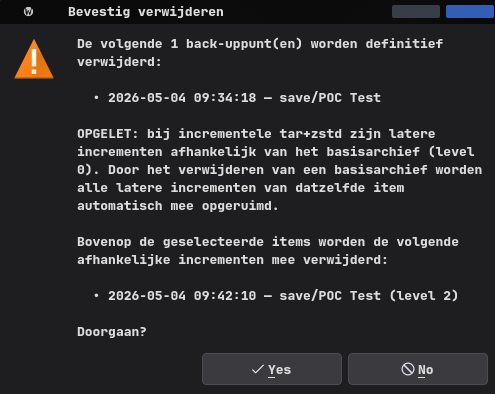
\includegraphics[width=0.55\linewidth]{verwijderen_van_een_level_0.png}
    \caption{Bevestigingsdialoog bij het verwijderen van een level-0-basisarchief. De dialoog toont expliciet welke afhankelijke incrementen mee zullen worden opgeruimd, zodat de gebruiker geen verrassingen krijgt na bevestiging.}
    \label{fig:eval-delete-dialog}
\end{figure}

\section{Conformiteitscheck tegen de ontwerprichtlijnen}
\label{sec:eval-conformiteit}

In het vorige hoofdstuk werden elf ontwerprichtlijnen geformuleerd op basis van de technische analyse. Tabel~\ref{tab:eval-conformiteit} geeft een beknopt overzicht van de implementatiestatus van elke richtlijn in het huidige prototype. De daaropvolgende toelichting behandelt enkel de richtlijnen die nuance vereisen.

\begin{table}[h]
    \centering
    \caption{Conformiteit van het prototype met de ontwerprichtlijnen.}
    \label{tab:eval-conformiteit}
    \small
    \begin{tabular}{p{0.04\linewidth}p{0.40\linewidth}p{0.18\linewidth}p{0.25\linewidth}}
        \toprule
        \textbf{\#} & \textbf{Richtlijn} & \textbf{Status} & \textbf{Toelichting} \\
        \midrule
        1 & Snapshot primair op btrfs              & Niet geïmplementeerd & Uitbreiding \\
        2 & Incrementele tar+zstd als alternatief  & Volledig             & Kernimplementatie \\
        3 & Differentieel afgeraden                & Conform              & Geen optie aangeboden \\
        4 & Volledige back-up zelden zinvol        & Conform              & Level 0 dient enkel als basis \\
        5 & \texttt{zstd} standaard                & Volledig             & Kernimplementatie \\
        6 & \texttt{xz} optioneel voor max. opslag & Niet geïmplementeerd & Uitbreiding \\
        7 & Andere algoritmes afgeraden            & Conform              & Geen optie aangeboden \\
        9 & Lokaal werken, geen netwerk            & Volledig             & Geen netwerklogica \\
        10 & Methode en compressie orthogonaal     & Conform              & Architectuur scheidt beide \\
        11 & Voorspelbaarheid als ontwerpkwaliteit & Volledig             & Methode zichtbaar in UI, sets gegroepeerd, huidige status zichtbaar \\
        \bottomrule
    \end{tabular}
\end{table}

\paragraph{Richtlijn 1: Snapshotting als uitbreiding.}
De technische analyse heeft btrfs-snapshotting aangeduid als de primaire methode voor opstellingen die het ondersteunen. In de finale tool werd deze methode echter weggelaten. Het percentage computergebruikers dat een btrfs-bestandssysteem gebruikt is bijzonder laag, en de typische KSP-speler bevindt zich op Windows met NTFS of op een Linux-systeem met ext4. Snapshotting heeft daardoor een beperkte praktische relevantie voor de doelgroep, ondanks de gunstige technische eigenschappen. Btrfs-snapshotting wordt om die reden behandeld als een uitbreiding in plaats van een kernvereiste. Het prototype valt voor alle bestandssystemen terug op de tweede aanbeveling uit de analyse: incrementele tar+zstd.

\paragraph{Richtlijn 6: \texttt{xz} als uitbreiding.}
De tool gebruikt momenteel uitsluitend \texttt{zstd} als compressie-algoritme, conform richtlijn~5. Een optionele variant met \texttt{xz} voor gebruikers die maximale opslagbesparing wensen werd nog niet geïmplementeerd. Het toevoegen van een tweede algoritme-keuze in de configuratie-tab is technisch eenvoudig en wordt beschouwd als een gepaste uitbreiding.


\section{Heuristische evaluatie van de gebruikersinterface}
\label{sec:eval-heuristiek}

De bruikbaarheid van de UI werd beoordeeld via een heuristische evaluatie volgens de tien principes van Nielsen. Per principe wordt kort vermeld hoe het prototype ermee omgaat, met een lichte status (sterk, voldoende of aandachtspunt).

\begin{description}
    \item[Zichtbaarheid van systeemstatus: sterk.] De progressbar en live log tijdens een back-up of restore tonen duidelijk welke operatie aan de gang is. De groene cirkel naast het huidige back-uppunt informeert over de actieve toestand. De gekozen back-upmethode wordt rechtsbovenin de back-up-tab permanent zichtbaar gehouden.
    \item[Match met de echte wereld: sterk.] Begrippen als ``back-up maken'', ``herstellen'' en ``installatie toevoegen'' sluiten aan bij gangbaar taalgebruik van eindgebruikers. Technische termen zoals \texttt{btrfs} of \texttt{snar} blijven achter de schermen.
    \item[Gebruikerscontrole en vrijheid: voldoende.] Bevestigingsdialogen vóór restore en delete voorkomen accidentele onomkeerbare acties. Een ``ongedaan maken''-functie ontbreekt: eens een restore is uitgevoerd, kan de gebruiker enkel terugvallen op een ander back-uppunt.
    \item[Consistentie en standaarden: sterk.] De Qt/KDE- look-and-feel zorgt voor herkenbaar gedrag van knoppen, dialogen en lijsten. Acties die data wijzigen krijgen consistent een blauwe (primaire) of rode (gevaarlijke) accentkleur.
    \item[Foutpreventie: sterk.] Stock-content wordt automatisch uitgesloten van de mod-lijst, waardoor de gebruiker geen onnodige back-ups kan maken van data die niet vervangen mag worden. De cascade-waarschuwing bij het verwijderen van een level 0 (figuur~\ref{fig:eval-delete-dialog}) toont expliciet de afhankelijkheden vóór bevestiging.
    \item[Herkennen in plaats van onthouden: voldoende.] Back-uppunten zijn gegroepeerd per back-up-actie en daarbinnen per type. De gebruiker hoeft geen IDs of timestamps te onthouden, het visueel herkennen van een set en het aanvinken van items volstaat. De mogelijkheid om een naam te geven aan een back-up ontbreekt nog.
    \item[Flexibiliteit en efficiëntie: voldoende.] Knoppen voor ``alles selecteren'' en ``niets selecteren'' versnellen bulk-operaties. De boomstructuur kan in zijn geheel uitgevouwen of opgevouwen worden. Sneltoetsen voor frequente acties ontbreken.
    \item[Esthetisch en minimalistisch ontwerp — sterk.] De UI bestaat uit drie tabs zonder overbodige elementen. Hint-teksten verschijnen enkel waar de gebruiker context nodig heeft.
    \item[Foutdiagnose: voldoende.] Foutmeldingen verschijnen in de log onderaan en in een dialoog. Voor een PoC is dit voldoende, maar uitgebreidere foutclassificatie (bijvoorbeeld onderscheid tussen ``schijf vol'' en ``rechten ontbreken'') zou de gebruiksvriendelijkheid in productie verhogen.
    \item[Hulp en documentatie: aandachtspunt.] De tool bevat enkel hint-labels per tab. Een aparte help-pagina, tooltip-uitleg op individuele velden of een korte introductie-tour ontbreekt. Voor een PoC is de tool eenvoudig genoeg om dit te aanvaarden, maar voor productiekwaliteit is documentatie een nodige toevoeging.
\end{description}

Een heuristische evaluatie door de ontwikkelaar zelf vangt blinde vlekken niet op die echte gebruikers wel zouden ontdekken. Deze sectie biedt daarom een gestructureerde reflectie op de UI-kwaliteit, geen gevalideerde usability-meting. Voor een productieversie zou gebruikersonderzoek met effectieve KSP-spelers een logische volgende stap zijn.


\section{Beperkingen en aanknopingspunten voor toekomstig werk}
\label{sec:eval-toekomst}

Onderstaande punten geven aan welke aspecten buiten scope zijn gehouden en hoe zij in toekomstig werk kunnen worden aangepakt.

\paragraph{Geen evaluatie met externe testers.}
De UX-evaluatie steunt op een heuristische analyse door de ontwikkelaar zelf. Een gevalideerde usability-studie met effectieve KSP-spelers zou pas mogelijk zijn na een eerste distributie van de tool en valt buiten de scope van deze bachelorproef.

\paragraph{Btrfs-snapshotting.}
Zoals besproken in sectie~\ref{sec:eval-conformiteit} werd de snapshot-methode niet geïmplementeerd in de finale tool wegens de beperkte praktische relevantie voor de doelgroep. Voor gebruikers op een btrfs-systeem die het maximale uit hun bestandssysteem willen halen, blijft dit een goede uitbreiding.

\paragraph{\texttt{xz} als optionele compressie.}
De tool gebruikt momenteel uitsluitend \texttt{zstd}. Een configuratie-optie waarmee de gebruiker kan kiezen voor \texttt{xz} wanneer maximale opslagbesparing is gewild zou conform richtlijn~6 zijn en is technisch eenvoudig toe te voegen.

\paragraph{automatische opruim.}
Het prototype voorziet geen automatisch beheer van oude back-uppunten. Bij langdurig gebruik kan de hoeveelheid back-uppunten oplopen. Een mechanisme dat oudere punten verwijdert volgens een instelbare  optie, zou de opslagvoetafdruk op lange termijn beheersbaar houden.

\paragraph{Scheduling van automatische back-ups.}
Op dit moment maakt de gebruiker manueel een back-up via de back-up-tab. Een planning-mechanisme dat automatisch een back-up maakt vlak vóór een mod-update of op vaste tijdstippen, sluit aan bij het oorspronkelijke gebruiksscenario en is een logische uitbreiding.

\paragraph{Multi-game-ondersteuning.}
Het prototype ondersteunt enkel KSP. De architectuur is generiek genoeg om uitgebreid te worden naar andere mod-gebaseerde games.

\paragraph{Integratie in een modlauncher.}
Het ultieme doel van een back-upsysteem zoals dit is rechtstreekse integratie in een bestaande modlauncher. Voor KSP betekent dit een integratie in CKAN. Aangezien CKAN geschreven is in C\#, vraagt deze integratie een herschrijving van de tool in c\#. Dit valt buiten de scope van het prototype en wordt beschouwd als de volgende stap naar een volwaardig back-up systeem.


\section{Samenvatting}
\label{sec:eval-samenvatting}

De evaluatie heeft het prototype op drie dimensies onderzocht: functionele correctheid, conformiteit met de ontwerprichtlijnen, en bruikbaarheid van de gebruikersinterface. De testmatrix bevestigt dat de tool zijn gedragsspecificatie nakomt over twintig testgevallen, gegroepeerd in vier clusters, inclusief edge cases zoals de cascade-cleanup bij het verwijderen van een basisarchief. De conformiteitscheck toont dat zes van de tien besproken richtlijnen volledig zijn geïmplementeerd, drie conform zijn afgehandeld door bewust geen optie aan te bieden, en twee (snapshotting en \texttt{xz}) als gemotiveerde uitbreiding voor toekomstig werk zijn aangemerkt. De heuristische UI-evaluatie identificeert het prototype als bruikbaar binnen de PoC-context, met enkele aandachtspunten waarvan de belangrijkste (documentatie, sneltoetsen, ``ongedaan maken'') typisch onder productiekwaliteit horen.

Een positieve observatie tijdens de evaluatie was dat het prototype probleemloos werkt op realistische werklasten: indicatieve metingen op een KSP-installatie van 20{,}5~GB met 113 mods leverden een back-uptijd van ongeveer 37{,}5~seconden en een restoretijd van ongeveer 25~seconden op, terwijl de UI gedurende de hele operatie responsief bleef. Het prototype demonstreert daarmee dat de in deze bachelorproef geformuleerde ontwerprichtlijnen niet alleen theoretisch verdedigbaar zijn, maar ook praktisch realiseerbaar in een eenvoudige Linux-applicatie die vandaag al bruikbaar is voor de oorspronkelijke gebruikssituatie.

%%=============================================================================
%% Conclusie
%%=============================================================================

\chapter{Conclusie}%
\label{ch:conclusie}

\section{Antwoorden op de onderzoeksvragen}
\label{sec:concl-deelvragen}

Om tot een gestructureerd antwoord op de hoofdvraag te komen, worden eerst de vijf deelvragen kort beantwoord op basis van wat in de voorgaande hoofdstukken werd onderzocht.

\subsection*{Deelvraag 1: Welke oplossingen worden vandaag toegepast om kapotte installaties of corrupte savegames te herstellen, en welke beperkingen vertonen ze?}

De analyse van zevenenveertig posts uit de KSP-community leverde een consistent beeld op. De meest voorgestelde oplossing voor crashes en modconflicten is een volledige herinstallatie van de \texttt{GameData}-map: alle mods verwijderen, de spelintegriteit via Steam verifiëren en mods opnieuw installeren. Voor corrupte savegames is de beste oplossing het manueel hernoemen van een back-upbestand in \texttt{/saves/<savegame>/Backup} naar \texttt{persistent.sfs}. Beide oplossingen werken in principe, maar hebben aanzienlijke beperkingen. Een herinstallatie is destructief en tijdrovend: alle configuratie en mod-aanpassingen gaan verloren. Het manueel herstellen van een save vereist dat de gebruiker weet dat de back-upmap bestaat, wat in de praktijk zelden het geval blijkt te zijn. Een vroege poging tot een geautomatiseerde oplossing, Jebretary, dateert uit 2014 en werd sindsdien niet meer onderhouden. Het feit dat geen volwaardige opvolger is verschenen en dat gebruikers vandaag nog steeds dezelfde handmatige procedures moeten doorlopen, bevestigt dat dit een structureel onopgelost probleem is.

\subsection*{Deelvraag 2: Welke vormen van dataverlies en corruptie komen het vaakst voor bij modlaunchers zonder ingebouwd back-up- of rollbackmechanisme?}

Vier categorieën komen naar voren als de meest voorkomende. Crashes door modconflicten, verouderde mods of ontbrekende afhankelijkheden vormen de grootste groep en leiden vaak tot een onbruikbare installatie waarbij zelfs een herinstallatie van de specifieke mod het probleem niet oplost, omdat overlappende configuratiebestanden achterblijven. Beschadigde of verloren savegames vormen de tweede categorie, met als centrale oorzaak een corrupte \texttt{persistent.sfs} door stroomuitval, een crash, een KSP-automatische update tijdens actieve vluchten of een antivirusprogramma dat het bestand verwijdert. De derde categorie betreft mods die geïnstalleerd worden maar niet zichtbaar zijn in het spel, doorgaans door gebruikersfouten zoals een verkeerde installatielocatie. Een vierde, minder zichtbare categorie betreft geheugentekorten die zich manifesteren als willekeurige crashes zonder duidelijke foutmelding.

\subsection*{Deelvraag 3: Welke technische methoden bestaan er om efficiënte back-up- en rollbacksystemen te implementeren in softwaretoepassingen?}

De technische analyse heeft vier methodes vergeleken op basis van metingen: volledige back-up, incrementele back-up, differentiële back-up en copy-on-write snapshotting via btrfs. Voor elk van deze methodes zijn de eigenschappen op het vlak van snelheid, opslaggebruik, CPU-belasting en geheugengebruik gemeten op realistische werklasten met savegames en mods. Daarnaast werden zeven compressie-algoritmes vergeleken: \texttt{gzip}, \texttt{bzip2}, \texttt{xz}, \texttt{lzma}, \texttt{lzip}, \texttt{lzop} en \texttt{zstd}. De analyse heeft duidelijk gemaakt dat geen enkele methode of algoritme universeel optimaal is, elke keuze brengt een afweging met zich mee tussen back-uptijd, restoretijd, opslagvoetafdruk en systeembelasting.

\subsection*{Deelvraag 4: Welke aanpak biedt de beste balans tussen opslagruimte, snelheid en computer resourcegebruik voor het back-uppen van grote modinstallaties?}

In praktisch elk scenario is de snapshotmethode op btrfs technisch het meest aantrekkelijk: het combineert constante back-upkost, quasi-instantane rollbacks en lage fysieke opslagvoetafdruk dankzij blokniveau-deduplicatie. Wanneer btrfs niet beschikbaar is, biedt incrementele tar in combinatie met \texttt{zstd}-compressie de beste afweging. \texttt{zstd} bleek in de metingen op grote werklasten zelfs sneller dan ongecomprimeerde tar, doordat de multithreaded compressie de extra rekentijd ruimschoots compenseert door de verminderde I/O-belasting van een kleiner archief. De vermindering van het opslaggebruik bedraagt voor de geteste modset ongeveer 53 procent ten opzichte van de ongecomprimeerde back-up, terwijl de back-uptijd zelfs licht lager ligt.

\subsection*{Deelvraag 5: Hoe kan een dergelijk systeem gebruiksvriendelijk en effectief geïmplementeerd worden in een tool?}

Het ontwikkelde prototype demonstreert dat de geformuleerde ontwerprichtlijnen praktisch realiseerbaar zijn in een eenvoudige applicatie. De tool combineert drie functionele kerntaken (back-ups maken, herstellen en beheren) in een interface met drie tabbladen. Gebruiksvriendelijkheidskeuzes betreffen het groeperen van back-uppunten per back-up-actie en daarbinnen per type, een visuele aanduiding van het huidige back-uppunt per item, expliciete bevestigingsdialogen vóór onomkeerbare acties, en asynchrone uitvoering zodat de gebruikersinterface ook tijdens back-ups van meerdere gigabytes responsief blijft. De evaluatie bevestigt dat het prototype deze functionaliteit op realistische werklasten correct uitvoert: een back-up van een KSP-installatie van 20{,}5 GB met 113 mods voltooit in ongeveer 37{,}5 seconden, terwijl een volledige restore in ongeveer 25 seconden afgehandeld wordt.


\section{Antwoord op de hoofdvraag}
\label{sec:concl-hoofdvraag}

De centrale onderzoeksvraag van deze bachelorproef luidde:

\begin{quote}
    \emph{Hoe kan een robuust en efficiënt back-up- en rollbackmechanisme worden ontworpen voor modlaunchers zoals CKAN, zodat dataverlies en corruptie voorkomen kunnen worden zonder negatieve impact op performantie of gebruiksvriendelijkheid?}
\end{quote}

Het antwoord dat uit dit onderzoek voortkomt, kan in vier kernpunten worden samengevat.

\paragraph{Een gelaagde methodekeuze afhankelijk van het bestandssysteem.}
Geen enkele back-upmethode is universeel optimaal. Op bestandssystemen die copy-on-write snapshots ondersteunen (zoals btrfs of zfs) levert de snapshotmethode de beste resultaten op alle geëvalueerde dimensies. Op andere bestandssystemen biedt incrementele tar in combinatie met \texttt{zstd}-compressie de beste afweging tussen snelheid, opslag en betrouwbaarheid. Een robuust systeem detecteert het beschikbare bestandssysteem en kiest automatisch de meest geschikte methode, met de mogelijkheid voor de gebruiker om zelf een keuze op te leggen wanneer beide methodes beschikbaar zijn.

\paragraph{Compressie als integraal onderdeel van het ontwerp.}
De analyse heeft aangetoond dat een goed gekozen compressie-algoritme de opslagvoetafdruk significant kan verminderen zonder de back-up-prestaties negatief te beïnvloeden. \texttt{zstd} springt hier consistent uit als de meest evenwichtige keuze. Voor gebruikers die de allerkleinste archieven willen, blijft \texttt{xz} een alternatief, indien de hogere geheugenvoetafdruk acceptabel is. Andere algoritmes leveren in de geteste werklasten geen meetbaar voordeel op en zijn voor de doelgroep niet relevant.

\paragraph{Lokaal werken als ontwerpprincipe.}
Voor de specifieke context van modlaunchers, waarbij de eindgebruiker het spel offline kan spelen en mods uit enkele gigabytes kunnen bestaan, is een lokaal back-upsysteem superieur aan een cloud-gebaseerde oplossing. Het back-upmechanisme moet kunnen opereren zonder netwerkverbinding en mag geen grote vertragingen introduceren in de gaming sessies van de gebruiker.

\paragraph{Voorspelbaarheid en zichtbaarheid in de gebruikersinterface.}
De gebruiksvriendelijkheid van een back-upsysteem hangt niet alleen af van technische snelheid, maar ook van de mate waarin de gebruiker inzicht heeft in wat er gebeurt. Het prototype illustreert dit door de gekozen methode permanent zichtbaar te maken, back-uppunten gegroepeerd per actie weer te geven, het huidige actieve punt visueel te markeren, en bevestigingsdialogen te tonen vóór onomkeerbare acties.

Samen bieden deze vier kernpunten een onderbouwd antwoord op de hoofdvraag: een back-up- en rollbackmechanisme voor modlaunchers combineert een gelaagde methodekeuze met efficiënte compressie, draait lokaal en plaatst voorspelbaarheid centraal in de gebruikersinterface. Het ontwikkelde prototype toont dat deze combinatie technisch realiseerbaar is en in de praktijk op realistische werklasten functioneert.


\section{Bijdrage en meerwaarde}
\label{sec:concl-bijdrage}

De bijdrage van dit onderzoek aan het vakgebied bestaat uit drie delen. Ten eerste levert de probleemanalyse een gestructureerd overzicht van de meest voorkomende vormen van dataverlies en corruptie in de KSP-community, op basis van een dataset die twaalf jaar aan posts overspant. Hieruit blijkt dat het probleem structureel is en wijdverspreid, en dat de gangbare oplossingen beperkt en gebruikersonvriendelijk blijven.

Ten tweede levert de technische analyse een onderbouwde vergelijking van back-upmethodes en compressie-algoritmes binnen de specifieke context van modlauncher-werklasten. Deze vergelijking verschilt van klassieke back-upliteratuur doordat het gericht is op twee zeer verschillende soorten data: kleine, zeer comprimeerbare savegames en grote, reeds deels gecomprimeerde mod-assets. En doordat het de afwegingen evalueert in het licht van een specifieke gebruikssituatie waarin een back-upactie vlak vóór een mod-update plaatsvindt en een rollback in een tijdsdrukscenario gebeurt.

Ten derde resulteren de twee analyses samen in een concrete set van ontwerprichtlijnen die direct toepasbaar zijn bij het ontwikkelen of uitbreiden van een modlauncher. Het prototype demonstreert dat deze richtlijnen ook praktisch realiseerbaar zijn en bewijst dat een gebruiksvriendelijk back-upsysteem voor modlaunchers vandaag al mogelijk is met bestaande tools.

Voor de doelgroep, de KSP-community in het bijzonder en modlauncher-gebruikers in het algemeen, biedt dit onderzoek de basis voor een concrete oplossing voor een probleem dat al meer dan een decennium structureel onopgelost is gebleven. De hoop is dat de ontwerprichtlijnen en het prototype een aanzet kunnen vormen voor een productiekwaliteit-implementatie, idealiter geïntegreerd in een bestaande modlauncher zoals CKAN.


\section{Kritische reflectie}
\label{sec:concl-reflectie}

Een aantal observaties tijdens dit onderzoek verdienen kritische reflectie, omdat ze niet vanzelfsprekend waren of de eerste verwachtingen gedeeltelijk hebben bijgesteld.

\paragraph{De goede prestaties van \texttt{zstd}.}
Bij aanvang van het onderzoek werd verwacht dat compressie steeds een afweging zou opleveren tussen back-uptijd en archiefgrootte, een snellere compressie betekent doorgaans een groter archief. \texttt{zstd} bleek deze afweging echter grotendeels te omzeilen op grote werklasten: in de metingen op de moddataset comprimeerde \texttt{zstd} zelfs sneller dan een ongecomprimeerde \texttt{tar}, doordat de multithreaded compressie de extra rekentijd compenseerde door de verminderde I/O-belasting van een kleiner archief. Dit was geen verwacht resultaat en heeft de aanbevelingen op dit punt sterker gemaakt dan oorspronkelijk geanticipeerd: \texttt{zstd} hoeft niet als compromis tussen snelheid en compressie te worden gepresenteerd, maar als een methode die in beide dimensies wint.

\paragraph{Mods comprimeren slechter dan savegames.}
Een tweede onverwachte vaststelling betrof de meer beperkte compressiewinst op de moddataset. Waar savegames met een ratio van ongeveer 0{,}07 gecomprimeerd konden worden, bleven alle algoritmes op de mods steken rond een ratio van 0{,}37 tot 0{,}54. De oorzaak ligt in het feit dat moderne mods grotendeels uit reeds gecomprimeerde assets bestaan: texturen, audio, modellen. Hoewel deze observatie technisch evident is achteraf, was het vooraf niet expliciet vermeld in de literatuur die werd geraadpleegd. De implicatie is praktisch relevant: voor mods levert een agressief algoritme zoals \texttt{xz} of \texttt{lzip} weinig extra winst op ten opzichte van een snel algoritme zoals \texttt{zstd}, terwijl de tijdkost sterk toeneemt.

\paragraph{Differentieel werd volledig gedomineerd door incrementeel.}
In de back-upliteratuur worden differentiële en incrementele back-ups vaak naast elkaar gepresenteerd als twee gelijkwaardige alternatieven met elk hun eigen voordelen. De empirische metingen in dit onderzoek nuanceren dat beeld: voor de geteste werklasten biedt differentieel geen meetbaar voordeel ten opzichte van incrementeel. De back-uptijd is hoger, het opslaggebruik is groter, en de restoretijd is nauwelijks beter. De theoretische voordelen van differentieel, een eenvoudigere restore omdat slechts twee archieven nodig zijn, wegen in de praktijk niet op tegen de nadelen. Voor het ontwerp van een back-upsysteem voor modlaunchers betekent dit dat de keuze tussen beide methodes minder open ligt dan eerder verwacht.

\paragraph{De keuze om btrfs-snapshotting niet in de finale tool op te nemen.}
Hoewel de technische analyse btrfs-snapshotting aanbeveelt als primaire methode op ondersteunde bestandssystemen, werd deze methode in de finale versie van het prototype niet meegenomen. De reden ligt niet bij de techniek zelf maar bij de doelgroep: het percentage computergebruikers dat een btrfs-bestandssysteem heeft is bijzonder laag, waardoor de praktische relevantie van deze methode voor de gemiddelde KSP-speler beperkt is.


\section{Vragen voor verder onderzoek}
\label{sec:concl-verder-onderzoek}

Het onderzoek heeft een aantal vragen opgeworpen die buiten de scope van deze bachelorproef vielen, maar die uitnodigen tot verder werk.

\paragraph{Hoe goed schaalt het systeem bij langdurig gebruik?}
Het prototype voorziet geen automatisch retentiebeleid. Bij langdurig gebruik kan de hoeveelheid back-uppunten en de bijhorende opslagvoetafdruk oplopen. Een onderzoek naar geautomatiseerde consolidatiestrategieën, bijvoorbeeld het periodiek samenvoegen van een keten incrementen tot een nieuwe basis-back-up, zou een waardevolle aanvulling vormen.

\paragraph{Hoe goed werkt snapshotting in de praktijk?}
Hoewel btrfs-snapshotting niet in de finale tool werd opgenomen, blijft het technisch een interessante optie voor gebruikers die hun KSP-installatie wel op btrfs hebben staan. Een verdere exploratie zou kunnen onderzoeken hoe een tool de gebruiker kan begeleiden bij het omzetten van een bestaande KSP-folder naar een volwaardige subvolume, zonder dat dit voor de eindgebruiker als ingrijpend overkomt. Een vergelijkbare vraag stelt zich voor zfs.

\paragraph{Hoe ziet integratie in CKAN er concreet uit?}
Het ultieme doel van een back-upsysteem voor KSP-modding is een integratie in de bestaande modlauncher. CKAN is geschreven in C\#, wat een herschrijving of port van het back-upmechanisme zou vereisen. Een vervolgonderzoek zou kunnen vaststellen welke architecturale aanpassingen aan CKAN noodzakelijk zijn om een back-uphook in te bouwen, en welke onderdelen van de hier ontwikkelde Python-implementatie rechtstreeks vertaalbaar zijn.

\paragraph{Hoe generaliseren de bevindingen naar andere games?}
KSP is een specifieke casus, maar de problemen die in de probleemanalyse werden geïdentificeerd zijn niet exclusief voor KSP. Modlaunchers bestaan ook voor games zoals Minecraft, Skyrim, Fallout en vele andere. Een vergelijkende studie zou kunnen vaststellen in welke mate de hier voorgestelde ontwerprichtlijnen overdraagbaar zijn naar andere mod-ecosystemen, en waar context-specifieke aanpassingen noodzakelijk blijven.

\bigskip

Het onderzoek heeft daarmee niet alleen een antwoord geformuleerd op de oorspronkelijke onderzoeksvraag, maar ook nieuwe richtingen geopend voor toekomstig werk. Dat een meer dan tien jaar oud probleem in een actieve gamingcommunity vandaag nog steeds structureel onopgelost is, suggereert dat zowel de onderzoeksvragen als de ontwerprichtlijnen die in deze bachelorproef zijn geformuleerd, ook na deze proef relevant zullen blijven.




%---------- Bijlagen -----------------------------------------------------------

\appendix

\chapter{Onderzoeksvoorstel}

Het onderwerp van deze bachelorproef is gebaseerd op een onderzoeksvoorstel dat vooraf werd beoordeeld door de promotor. Dat voorstel is opgenomen in deze bijlage.

%% TODO: 
%\section*{Samenvatting}

% Kopieer en plak hier de samenvatting (abstract) van je onderzoeksvoorstel.

% Verwijzing naar het bestand met de inhoud van het onderzoeksvoorstel
\input{../voorstel/voorstel-inhoud}

%%---------- Andere bijlagen --------------------------------------------------
\chapter{geanalyseerde community-posts}
\label{app:corpus}

De onderstaande links verwijzen naar de forum-posts, Reddit-threads en Steam-discussies die zijn geanalyseerd in hoofdstuk~\ref{ch:probleemanalyse} van dit onderzoek. De posts zijn ingedeeld per platform.

\section{Reddit}

\begin{itemize}
  \item \url{https://www.reddit.com/r/KerbalSpaceProgram/comments/1jngysk/need_to_reinstall_after_a_botched_mod_update_what/}
  \item \url{https://www.reddit.com/r/KerbalSpaceProgram/comments/1ndnng9/so_i_need_more_help_with_my_install/}
  \item \url{https://www.reddit.com/r/KerbalSpaceProgram/comments/xh4g68/hello_today_i_decided_to_reinstall_kerbal_keeps/}
  \item \url{https://www.reddit.com/r/KerbalSpaceProgram/comments/1oyew0g/mods_not_working/}
  \item \url{https://www.reddit.com/r/KerbalSpaceProgram/comments/1fu621n/adding_any_mods_crashes_game/}
  \item \url{https://www.reddit.com/r/KerbalSpaceProgram/comments/1cu9dyc/is_mechjeb_broken/}
  \item \url{https://www.reddit.com/r/KerbalSpaceProgram/comments/1pcczgv/modding_issues_really_need_help/}
  \item \url{https://www.reddit.com/r/KerbalAcademy/comments/hh2nbd/ksp_crashes_on_start_when_using_mods_installed/}
  \item \url{https://www.reddit.com/r/KerbalSpaceProgram/comments/10obqhc/environmental_visual_enhancements_mod_not_working/}
  \item \url{https://www.reddit.com/r/KerbalSpaceProgram/comments/1q9ogc2/game_crashes_during_loading_or_just_after_loading/}
  \item \url{https://www.reddit.com/r/KerbalSpaceProgram/comments/1kd621v/my_game_crashes_when_i_open_my_save_game_actually/}
  \item \url{https://www.reddit.com/r/KerbalSpaceProgram/comments/sd5yzo/ksp_crashing_moments_after_launch_before_loading/}
  \item \url{https://www.reddit.com/r/KerbalSpaceProgram/comments/crpkwx/game_crashes_during_startup/}
  \item \url{https://www.reddit.com/r/KerbalSpaceProgram/comments/1myr6zv/what_mod_is_causing_my_game_to_crash_log_in/}
  \item \url{https://www.reddit.com/r/KerbalSpaceProgram/comments/14dxppr/lil_problem/}
\end{itemize}

\section{Steam Community}

\begin{itemize}
  \item \url{https://steamcommunity.com/app/220200/discussions/0/3177854919325291614}
  \item \url{https://steamcommunity.com/app/220200/discussions/0/620712999968397259/}
  \item \url{https://steamcommunity.com/app/220200/discussions/0/4343240135700589704/}
  \item \url{https://steamcommunity.com/app/220200/discussions/0/1698294337791135092/}
  \item \url{https://steamcommunity.com/app/220200/discussions/0/1489987634005482013/}
  \item \url{https://steamcommunity.com/app/220200/discussions/0/1698300679772676735/}
  \item \url{https://steamcommunity.com/app/220200/discussions/0/3080999687771184115/}
\end{itemize}

\section{KSP-forum}

\begin{itemize}
  \item \url{https://forum.kerbalspaceprogram.com/topic/225993-fatal-error-with-b9-parts-switch-mod-in-ksp-v11125-on-steam-mods-through-ckan}
  \item \url{https://forum.kerbalspaceprogram.com/topic/197082-ckan-mod-manager-for-ksp1-and-ksp2/page/25/}
  \item \url{https://forum.kerbalspaceprogram.com/topic/216841-crash-with-somewhat-extensive-modding-cause-unknown/}
  \item \url{https://forum.kerbalspaceprogram.com/topic/162662-ksp-keeps-crashing-with-mods-installed/}
  \item \url{https://forum.kerbalspaceprogram.com/topic/199854-ksp-fresh-install-crash/}
  \item \url{https://forum.kerbalspaceprogram.com/topic/226638-ksp-keeps-crashing-no-matter-if-i-have-mods-installed-or-not/}
  \item \url{https://forum.kerbalspaceprogram.com/topic/177238-ksp-143-keeps-crashing-can-anyone-help-me-diagnose-logs-problems/}
  \item \url{https://forum.kerbalspaceprogram.com/topic/225173-ksp-keeps-crashing/}
  \item \url{https://forum.kerbalspaceprogram.com/topic/171075-game-crashes-seems-to-be-caused-by-mods-not-sure-which-ones/}
  \item \url{https://forum.kerbalspaceprogram.com/topic/227877-strange-crash/}
  \item \url{https://forum.kerbalspaceprogram.com/topic/179092-b9-part-switch-forces-crash/}
  \item \url{https://forum.kerbalspaceprogram.com/topic/158448-gamedata-modification-issues/}
  \item \url{https://forum.kerbalspaceprogram.com/topic/90327-crash-log-with-mods-new-to-ksp-please-help/}
  \item \url{https://forum.kerbalspaceprogram.com/topic/199179-help-cant-understand-crash-log/}
  \item \url{https://forum.kerbalspaceprogram.com/topic/182044-crash-report-just-sharing/}
  \item \url{https://forum.kerbalspaceprogram.com/topic/220110-ksp-modded-crashes-after-fixed-times/}
  \item \url{https://forum.kerbalspaceprogram.com/topic/228297-getting-errors-when-loading-saved-game/}
  \item \url{https://forum.kerbalspaceprogram.com/topic/156312-deleted-persistentsfs/}
  \item \url{https://forum.kerbalspaceprogram.com/topic/92355-resume-saved-wont-work/}
  \item \url{https://forum.kerbalspaceprogram.com/topic/201156-save-incompatible/}
  \item \url{https://forum.kerbalspaceprogram.com/topic/162247-crash-and-curruped-savefile-after-switching-vessel-in-tracking-station-ksp130/}
  \item \url{https://forum.kerbalspaceprogram.com/topic/209697-save-corrupted-value-cannot-be-null/}
  \item \url{https://forum.kerbalspaceprogram.com/topic/110300-corrupt-save-file-recovery/}
  \item \url{https://forum.kerbalspaceprogram.com/topic/214907-ksp-save-file-slightly-corrupted/}
\end{itemize}

\section{Stack Exchange en GitHub}

\begin{itemize}
    \item \url{https://gaming.stackexchange.com/questions/381307/ksp-mods-not-loading-after-manual-install-win7}
    \item \url{https://github.com/Sujimichi/Jebretary}
\end{itemize}
\chapter{Testscripts}
\label{app:testscripts}

De vier Bash-scripts die zijn gebruikt voor de metingen in hoofdstuk~\ref{ch:technischeanalyse} worden hier weergegeven. Elk script accepteert twee argumenten: \texttt{backup} of \texttt{restore} als eerste argument, en het aantal herhaalde runs als tweede argument. Alle scripts schrijven hun resultaten weg naar een CSV-bestand in de \texttt{workspace/}-submap.

\section{\texttt{full.sh}: Volledige back-up}
\label{app:full-sh}

\inputminted[breakanywhere,fontsize=\small,frame=single]{bash}{scripts/full.sh}

\section{\texttt{incremental.sh}: incrementele back-up}
\label{app:incremental-sh}

\inputminted[breakanywhere,fontsize=\small,frame=single]{bash}{scripts/incremental.sh}

\section{\texttt{differential.sh}: differentiële back-up}
\label{app:differential-sh}

\inputminted[breakanywhere,fontsize=\small,frame=single]{bash}{scripts/differential.sh}

\section{\texttt{snapshot.sh}: snapshot back-up}
\label{app:snapshot-sh}

\inputminted[breakanywhere,fontsize=\small,frame=single]{bash}{scripts/snapshot.sh}

%%---------- Backmatter, referentielijst ---------------------------------------

\backmatter{}

\setlength\bibitemsep{2pt} %% Add Some space between the bibliograpy entries
\printbibliography[heading=bibintoc]

\end{document}
